% =====================================================================
% BMED365 (Spring 2027) — Lab 4: Differentiable Neurosymbolic AI Report
% Printable Companion Notebook Export: 00_isotropic_reslicing_and_polar_alignment.ipynb
% Compile with: pdflatex 00_isotropic_reslicing_and_polar_alignment_ipynb.tex (run twice)
% =====================================================================
\documentclass[10pt,a4paper]{article}

\usepackage[utf8]{inputenc}
\usepackage[T1]{fontenc}
\usepackage[english]{babel}
\usepackage{lmodern}
\usepackage{microtype}
\usepackage{graphicx}
\usepackage{booktabs}
\usepackage{xltabular}
\usepackage{tabularx}
\usepackage{array}
\usepackage[table]{xcolor}
\usepackage{amsmath,amssymb,mathtools}
\usepackage{enumitem}
\usepackage[margin=1.7cm,top=1.75cm,bottom=1.85cm,headheight=14pt]{geometry}
\usepackage{fancyhdr}
\usepackage{lastpage}
\usepackage{titlesec}
\usepackage[most]{tcolorbox}
\usepackage{listings}
\usepackage{float}
\usepackage{caption}
\usepackage[hyphens]{url}
\usepackage[
    colorlinks=true,
    linkcolor=uibblue,
    citecolor=uibblue,
    urlcolor=uibred,
    bookmarksnumbered=true,
    bookmarksopen=true,
    pdftitle={00_isotropic_reslicing_and_polar_alignment.ipynb -- Canonical Isotropic Reslicing and Polar N-S Alignment (BMED365 Spring 2027)},
    pdfauthor={Arvid Lundervold (University of Bergen & MMIV) -- BMED365 Spring 2027},
    pdfsubject={BMED365 Spring 2027 -- Differentiable Neurosymbolic AI Companion Notebook 00}
]{hyperref}
\def\UrlBreaks{\do\/\do-\do_\do.}
\let\origunderscore\_
\renewcommand{\_}{\origunderscore\allowbreak}

% =====================================================================
% COLORS (UiB / MMIV / BMED365 House Style)
% =====================================================================
\definecolor{uibblue}{RGB}{0, 61, 115}
\definecolor{uibred}{RGB}{175, 28, 44}
\definecolor{kiwigreen}{RGB}{27, 138, 90}
\definecolor{amberwarn}{RGB}{165, 95, 0}
\definecolor{amberbg}{RGB}{255, 250, 240}
\definecolor{lightgray}{RGB}{246, 248, 250}
\definecolor{rowalt}{RGB}{243, 247, 252}
\definecolor{codebg}{RGB}{245, 248, 252}
\definecolor{codehdr}{RGB}{224, 234, 246}
\definecolor{outbg}{RGB}{250, 250, 250}
\definecolor{outhdr}{RGB}{236, 238, 240}
\definecolor{codekw}{RGB}{0, 75, 145}
\definecolor{codestr}{RGB}{155, 35, 45}
\definecolor{codecmt}{RGB}{90, 105, 118}

% =====================================================================
% TYPOGRAPHY, HEADERS & CALLOUT BOXES
% =====================================================================
\setlength{\parindent}{0pt}
\setlength{\parskip}{0.42em}
\setlength{\emergencystretch}{1.8em}
\setlist[itemize]{topsep=2pt,itemsep=2pt,leftmargin=1.45em}
\setlist[enumerate]{topsep=2pt,itemsep=2pt,leftmargin=1.65em}

\newcolumntype{L}[1]{>{\raggedright\arraybackslash}p{#1}}
\newcolumntype{C}[1]{>{\centering\arraybackslash}p{#1}}
\newcolumntype{R}[1]{>{\raggedleft\arraybackslash}p{#1}}
\newcolumntype{Y}{>{\raggedright\arraybackslash}X}

\titleformat{\section}{\large\bfseries\color{uibblue}}{\thesection}{0.65em}{}[\vspace{1pt}\color{uibblue!40}\titlerule]
\titleformat{\subsection}{\normalsize\bfseries\color{uibblue!88!black}}{\thesubsection}{0.55em}{}
\titleformat{\subsubsection}{\small\bfseries\color{uibblue!75!black}}{\thesubsubsection}{0.5em}{}
\titlespacing*{\section}{0pt}{1.05em}{0.4em}
\titlespacing*{\subsection}{0pt}{0.75em}{0.25em}
\titlespacing*{\subsubsection}{0pt}{0.55em}{0.2em}

\pagestyle{fancy}
\fancyhf{}
\fancyhead[L]{\footnotesize\textcolor{gray}{BMED365 (Spring 2027) $\cdot$ Neurosymbolic 7\,T MRI Package}}
\fancyhead[R]{\footnotesize\textcolor{gray}{\texttt{00\_isotropic\_reslicing\_and\_polar\_alignment.ipynb}}}
\fancyfoot[L]{\footnotesize\textcolor{gray}{University of Bergen \& MMIV $\cdot$ \href{https://github.com/arvidl/BMED365-2027}{\textcolor{gray}{github.com/arvidl/BMED365-2027}}}}
\fancyfoot[R]{\footnotesize\textcolor{gray}{Page \thepage{} of \pageref{LastPage}}}
\renewcommand{\headrulewidth}{0.4pt}
\renewcommand{\footrulewidth}{0.2pt}

\fancypagestyle{firstpage}{
    \fancyhf{}
    \fancyfoot[L]{\footnotesize\textcolor{gray}{University of Bergen \& MMIV $\cdot$ \href{https://github.com/arvidl/BMED365-2027}{\textcolor{gray}{github.com/arvidl/BMED365-2027}}}}
    \fancyfoot[R]{\footnotesize\textcolor{gray}{Page \thepage{} of \pageref{LastPage}}}
    \renewcommand{\headrulewidth}{0pt}
    \renewcommand{\footrulewidth}{0.2pt}
}

\newtcolorbox{seqbox}[1][]{
    enhanced, breakable,
    colback=lightgray, colframe=uibblue,
    colbacktitle=uibblue, coltitle=white,
    fonttitle=\bfseries\small, title={#1},
    boxrule=0.6pt, arc=2.5pt, left=7pt, right=7pt, top=5pt, bottom=5pt
}

\newtcolorbox{codebox}[1][]{
    enhanced, breakable,
    colback=codebg, colframe=uibblue!35,
    colbacktitle=codehdr, coltitle=uibblue!90!black,
    fonttitle=\ttfamily\scriptsize\bfseries, title={#1},
    boxrule=0.55pt, arc=2.2pt, left=6pt, right=6pt, top=3pt, bottom=3pt,
    toptitle=2.5pt, bottomtitle=2.5pt
}

\newtcolorbox{outbox}[1][]{
    enhanced, breakable,
    colback=outbg, colframe=gray!45,
    colbacktitle=outhdr, coltitle=black!75,
    fonttitle=\ttfamily\scriptsize\bfseries, title={#1},
    boxrule=0.5pt, arc=2.2pt, left=6pt, right=6pt, top=3pt, bottom=3pt,
    toptitle=2pt, bottomtitle=2pt
}

\newtcolorbox{clinbox}[1][]{
    enhanced, breakable,
    colback=amberbg, colframe=amberwarn,
    colbacktitle=amberwarn, coltitle=white,
    fonttitle=\bfseries\small, title={#1},
    boxrule=0.6pt, arc=2.5pt, left=7pt, right=7pt, top=5pt, bottom=5pt
}

\newtcolorbox{guidehdr}[1][]{
    enhanced,
    colback=kiwigreen!6, colframe=kiwigreen!75!black,
    borderline west={2.5pt}{0pt}{kiwigreen!85!black},
    boxrule=0.45pt, arc=2pt, left=7pt, right=7pt, top=3.5pt, bottom=3.5pt,
    before skip=0.7em, after skip=0.35em
}

% --- Listings Styles (Full UTF-8 literate support for pdflatex) ---
\lstdefinestyle{pybmed}{
    language=Python,
    basicstyle=\ttfamily\scriptsize,
    keywordstyle=\bfseries\color{codekw},
    stringstyle=\color{codestr},
    commentstyle=\itshape\color{codecmt},
    showstringspaces=false,
    breaklines=true,
    breakatwhitespace=false,
    breakindent=12pt,
    columns=fullflexible,
    keepspaces=true,
    upquote=true,
    aboveskip=2pt,
    belowskip=2pt,
    xleftmargin=0pt,
    xrightmargin=0pt,
    literate={±}{{$\pm$}}1
             {³}{{\textsuperscript{3}}}1
             {²}{{\textsuperscript{2}}}1
             {¹}{{\textsuperscript{1}}}1
             {⁻}{{$^{-}$}}1
             {₀}{{$_{0}$}}1
             {₁}{{$_{1}$}}1
             {₂}{{$_{2}$}}1
             {•}{{$\bullet$}}1
             {×}{{$\times$}}1
             {°}{{$^\circ$}}1
             {′}{{$'$}}1
             {∘}{{$\circ$}}1
             {é}{{\'e}}1
             {ö}{{\"o}}1
             {Ł}{{\L{{}}}}1
             {Δ}{{$\Delta$}}1
             {α}{{$\alpha$}}1
             {θ}{{$\theta$}}1
             {–}{{--}}1
             {—}{{---}}1
             {−}{{-}}1
             {─}{{-}}1
             {≥}{{$\ge$}}1
             {≤}{{$\le$}}1
             {⊂}{{$\subset$}}1
             {∈}{{$\in$}}1
             {→}{{$\to$}}1
             {…}{{\ldots}}1
}

\lstdefinestyle{outbmed}{
    basicstyle=\ttfamily\scriptsize\color{black!85},
    showstringspaces=false,
    breaklines=true,
    breakatwhitespace=false,
    columns=fullflexible,
    keepspaces=true,
    upquote=true,
    aboveskip=1pt,
    belowskip=1pt,
    xleftmargin=0pt,
    xrightmargin=0pt,
    literate={±}{{$\pm$}}1
             {³}{{\textsuperscript{3}}}1
             {²}{{\textsuperscript{2}}}1
             {¹}{{\textsuperscript{1}}}1
             {⁻}{{$^{-}$}}1
             {₀}{{$_{0}$}}1
             {₁}{{$_{1}$}}1
             {₂}{{$_{2}$}}1
             {•}{{$\bullet$}}1
             {×}{{$\times$}}1
             {°}{{$^\circ$}}1
             {′}{{$'$}}1
             {∘}{{$\circ$}}1
             {Δ}{{$\Delta$}}1
             {θ}{{$\theta$}}1
             {–}{{--}}1
             {—}{{---}}1
             {−}{{-}}1
             {─}{{-}}1
             {≥}{{$\ge$}}1
             {≤}{{$\le$}}1
             {→}{{$\to$}}1
}

\newcommand{\ghblob}{https://github.com/arvidl/BMED365-2027/blob/main}
\newcommand{\colabbase}{https://colab.research.google.com/github/arvidl/BMED365-2027/blob/main}
\newcommand{\repodir}{Lab4-Comp-Imag/Kiwi-challenge/docs/neurosymbolic-report}
\newcommand{\colabbtn}[1]{%
  \href{#1}{\tcbox[on line, arc=2.5pt, boxsep=0pt, left=6pt, right=6pt, top=2.5pt, bottom=2.5pt,
    colback=amberwarn!85!yellow, colframe=white!70!amberwarn, boxrule=0.5pt]{%
    \sffamily\bfseries\scriptsize\color{white}Open in Google Colab}}%
}

% =====================================================================
\begin{document}
\thispagestyle{firstpage}

% --- TITLE BANNER ---
\begin{tcolorbox}[
    enhanced, colback=uibblue, colframe=uibblue,
    arc=3.5pt, left=12pt, right=12pt, top=9pt, bottom=9pt
]
{\Large\bfseries\color{white} Companion Notebook 00 --- Canonical Geometric Preprocessing ($f = f_2 \circ f_1$)\\[2pt]
{\large Isotropic Reslicing, Rigid Polar N--S Alignment, Invertibility \& 3-Seed Canonical OOD Ablation}}\\[4pt]
{\normalsize\color{white!90} BMED365 --- Computational Imaging, Modeling and AI in Biomedicine (Spring 2027)}\\[3pt]
{\footnotesize\color{white!84}
Arvid Lundervold (University of Bergen \& MMIV) $\;\cdot\;$ Formulated at Stilleskriving HKS (26/11-26) $\;\cdot\;$ Figs.\ 0a--0e $\;\cdot\;$ Measured runtime: \texttt{301.2 s} (MPS)
}\\[6pt]
\colabbtn{\colabbase/\repodir/notebooks/00_isotropic_reslicing_and_polar_alignment.ipynb}\hspace{8pt}
{\footnotesize\href{\ghblob/\repodir/notebooks/00_isotropic_reslicing_and_polar_alignment.ipynb}{\textcolor{white}{\underline{\texttt{00\_isotropic\_reslicing\_and\_polar\_alignment.ipynb} on GitHub}}}}\hspace{10pt}
{\footnotesize\href{\ghblob/\repodir/neurosymbolic-kiwi-report.pdf}{\textcolor{white}{\underline{Technical Report PDF}}}}
\end{tcolorbox}

\begin{seqbox}[Neurosymbolic 7\,T MRI Technical Report --- Companion Package (\texttt{docs/neurosymbolic-report})]
{\footnotesize Companion to \href{\ghblob/\repodir/neurosymbolic-kiwi-report.pdf}{\textbf{\texttt{neurosymbolic-kiwi-report.pdf}}} and shared library \href{\ghblob/\repodir/notebooks/kiwi_ns_lib.py}{\texttt{kiwi\_ns\_lib.py}} (\href{\ghblob/\repodir/notebooks/kiwi_ns_lib_py.pdf}{\textit{annotated PDF}}):}
\begin{enumerate}[start=0, itemsep=1.2pt, topsep=2pt, font=\footnotesize]
    \item \textbf{\texttt{00\_isotropic\_reslicing\_and\_polar\_alignment.ipynb} (this notebook)} --- Canonical geometric preprocessing $f = f_2 \circ f_1$ (isotropic reslicing + rigid N--S polar alignment), $f^{-1}$ invertibility on 98 Micro-GT \& 749 whole-fruit seeds, cylindrical Mercator atlas \& 3-seed + whole-organ OOD ablation (Figs.\ 0a--0e; 301.2\,s MPS).
    \item \href{\ghblob/\repodir/notebooks/01_data_geometry_and_prior_audit.ipynb}{\texttt{01\_data\_geometry\_and\_prior\_audit.ipynb}} --- 7\,T MRI geometry, empirical audit of Priors 1--3, tri-planar Micro-GT superimposition \& manual GT editing guide (Figs.\ 1--3, Table~3; 27.4\,s MPS).
    \item \href{\ghblob/\repodir/notebooks/02_instancenorm_trap_and_ltn_math.ipynb}{\texttt{02\_instancenorm\_trap\_and\_ltn\_math.ipynb}} --- Experimental proof of \texttt{InstanceNorm3d} coordinate erasure, Bayes Log-Odds \texttt{Organ-GPS}, fuzzy $T$-norms \& LTN $p$-mean autograd sweep (Figs.\ 4--5, Table~4; 7.2\,s MPS).
    \item \href{\ghblob/\repodir/notebooks/03_multiseed_ablation_and_calibration.ipynb}{\texttt{03\_multiseed\_ablation\_and\_calibration.ipynb}} --- 3-seed $\times$ 6-model controlled ablation, operating-point calibration shift \& unmasked whole-organ OOD safety (Figs.\ 6--7, Tables~5--6; 555.1\,s MPS).
    \item \href{\ghblob/\repodir/notebooks/04_mechanistic_interpretability_and_biomarkers.ipynb}{\texttt{04\_mechanistic\_interpretability\_and\_biomarkers.ipynb}} --- Causal neural--symbolic division of labor ($z_{\text{GPS}}$), Mat\'ern hard-core split sweep, error anatomy \& 128-slice NIfTI biomarkers (Figs.\ 8--9, Tables~7--8; 99.3\,s MPS).
    \item \href{\ghblob/\repodir/notebooks/05_axiom_stress_tests_and_clinical_translation.ipynb}{\texttt{05\_axiom\_stress\_tests\_and\_clinical\_translation.ipynb}} --- Pathological mass-effect center-shift ($\Delta r \in [0, 8]$\,mm) \& radial-scale ($\alpha \in [0.80, 1.25]$) stress tests vs.\ rigid post-hoc masks (Fig.\ 10, Table~9; 55.4\,s MPS).
\end{enumerate}
\end{seqbox}

\subsection*{Origin \& AI-Assisted Coding Provenance (From Sketch to Experiment)}
In keeping with BMED365's emphasis on \textbf{AI-assisted scientific coding and open-science provenance}, this notebook was seeded directly by the handwritten notepad sketch below (\textit{Stilleskriving HKS, 26/11-26}) paired with a single domain-grounded prompt (reproduced verbatim, preserving the original wording and light typos):

\begin{tcolorbox}[
    enhanced,
    colback=kiwigreen!4, colframe=kiwigreen!70!black,
    colbacktitle=kiwigreen!80!black, coltitle=white,
    fonttitle=\bfseries\small,
    title={Multimodal Human Seed: Handwritten Sketch + Verbatim Prompt (26/11-26, Stilleskriving HKS)},
    boxrule=0.55pt, arc=2.5pt, left=6pt, right=6pt, top=4pt, bottom=4pt,
    toptitle=2.5pt, bottomtitle=2.5pt
]
\noindent
\begin{minipage}[t]{0.34\linewidth}
    \vspace{0pt}
    \centering
    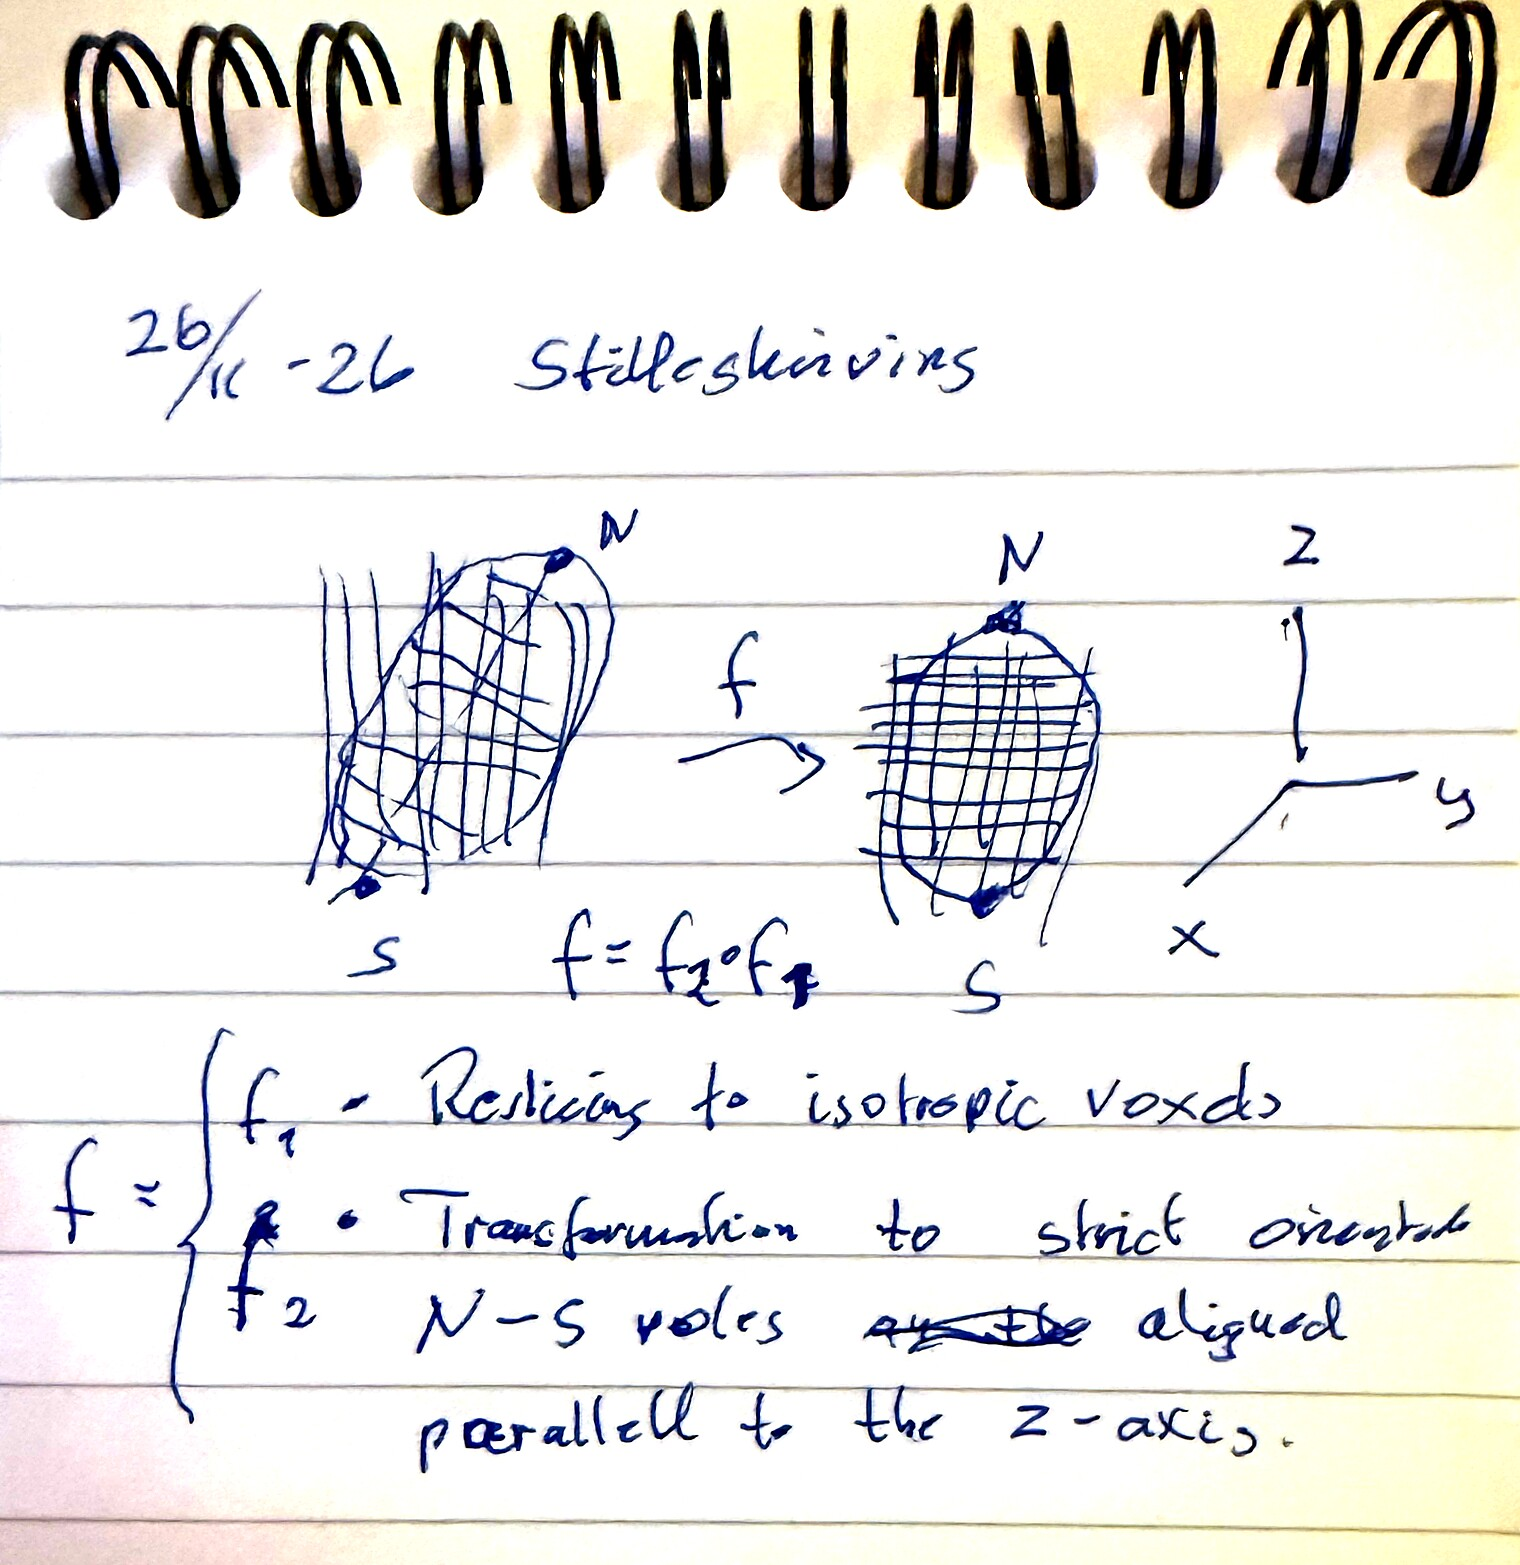
\includegraphics[width=\linewidth]{../figures/fig00_sketch_stilleskriving_20261126.jpg}\\[2pt]
    {\fontsize{7.0}{8.4}\selectfont\textit{Handwritten sketch (enhanced \& EXIF-stripped): $f = f_2 \circ f_1$ onto an isotropic N--S aligned grid.}\par}
\end{minipage}\hfill
\begin{minipage}[t]{0.63\linewidth}
    \vspace{0pt}
    {\fontsize{7.6}{9.1}\selectfont\textbf{Original Prompt (verbatim, 26/11-26):}\\[2pt]
    \textit{``In the relation to the Lab4 Kiwi-challenge I wnat to explore the following transformations (being sketched at Stilleskriving HKS 26/11-26 ). This relates to \url{https://github.com/arvidl/BMED365-2027/tree/main/Lab4-Comp-Imag/Kiwi-challenge/docs/neurosymbolic-report/notebooks} and a possible set of initial transformations of the intact 2005 UiB 7\,T Bruker Pharmascan RARE kiwifruit MRI (\texttt{256 $\times$ 256 $\times$ 128}, anisotropic voxel spacing \texttt{0.2344 $\times$ 0.2344 $\times$ 0.5000 mm\textsuperscript{3}}) with implications for the curated 3D Micro-Ground-Truth (\texttt{98} 3D seed instances). The idea behind these intitial transformation is to better deal with the seed segmentation problem (both manual segmentation and automated neurosymbolic segmentation) by making the voxels isotropic obtained by slice interpolation and reslicing along the long axis of the fruit, and then make an affine (rigid) transformation of the Kiwifruit object such that the (estimated) ``North pole'' and ``South pole'' is paralell to the z-axis in the intrisic coordinate system of the kiwi. By proper initial transformations and interpolation techniques - brining the origninal Kiwi recording into a new geometric representation - I thereby expect the manual and automated segmentation problem to be easier to perform and also visualize / evaluate. Eventually, the instance-segmented seeds can also be transformed back to the original Kiwi acquisition. If this is an interesting avenue to explore, please consider an implementation as a new Jupyter notebook 00 in Lab4-Comp-Imag/Kiwi-challenge/docs/neurosymbolic-report/notebooks.''}\par}
\end{minipage}
\end{tcolorbox}

\subsubsection*{Didactic Note --- What makes this human--AI workflow effective in biomedicine?}
\begin{itemize}[itemsep=1.5pt, topsep=2pt]
    \item \textbf{Domain scientist leads the formulation:} The human author supplies the physical acquisition insight (anisotropy + oblique bore tilt), the algebraic composition ($f = f_2 \circ f_1$), and the metrological requirement of \textbf{invertibility} ($f^{-1}$ back to native scanner coordinates) --- clear scientific thinking matters far more than polished prose.
    \item \textbf{High-signal context anchors:} Providing exact geometry (\texttt{256 $\times$ 256 $\times$ 128}, \texttt{0.2344 $\times$ 0.2344 $\times$ 0.5000 mm\textsuperscript{3}}), ground-truth scale (\texttt{98} seed instances), a visual sketch, and the exact repository path grounds the implementation in verifiable reality rather than generic boilerplate.
    \item \textbf{Hypothesis-testing rather than confirmation:} Open-ended framing (\textit{``If this is an interesting avenue to explore...''}) invites the AI coding collaborator to \textbf{empirically stress-test} the idea --- uncovering non-obvious pitfalls below (outer-mask PCA failing by $>17^\circ$, two-pass vs.\ single-pass pullback PSNR loss, anisotropic SDF artifacts, and the tilted-ROI prism caveat) rather than blindly confirming the hypothesis.
\end{itemize}

\subsection*{Scientific Motivation \& Transformation Hypothesis}
The archival 2005 UiB 7\,T Bruker Pharmascan RARE kiwifruit MRI (\texttt{256 $\times$ 256 $\times$ 128}) was acquired with \textbf{anisotropic voxels} ($0.2344 \times 0.2344 \times 0.5000\,\text{mm}^3$, slice-thickness aspect ratio $2.133:1$) and with the intact fruit resting obliquely tilted inside the scanner bore relative to the imaging $z$-axis. Before performing manual 3D curation or training automated neurosymbolic instance segmenters (Notebooks~\texttt{01}--\texttt{05}), we formalize, implement, and empirically audit a \textbf{two-stage geometric normalization} sketched at \textit{Stilleskriving HKS (26/11-26)}:
\[
f = f_2 \circ f_1 : \Omega_{\text{native}} \longrightarrow \Omega_{\text{canon}},
\]
where:
\begin{enumerate}
    \item \textbf{$f_1$ --- Isotropic Reslicing:} Maps the anisotropic $0.2344 \times 0.2344 \times 0.5000\,\text{mm}^3$ lattice onto an isotropic cubic lattice ($s_{\text{iso}} = 0.2344\,\text{mm}$ preserving native in-plane resolution $1:1$; also benchmarked against $0.30\,\text{mm}$ and $0.50\,\text{mm}$).
    \item \textbf{$f_2$ --- Rigid Polar Alignment ($R \in SO(3),\,\mathbf{t} \in \mathbb{R}^3$):} Estimates the fruit's intrinsic \textbf{North--South (N--S) polar axis} and rigidly aligns it strictly parallel to the canonical $z'$-axis ($u' = 0,\, v' = 0$), centering the equatorial plane at $z' = 0$.
    \item \textbf{Invertibility ($f^{-1} = f_1^{-1} \circ f_2^{-1}$):} Projects instance-segmented 3D seeds (both the \texttt{98} curated Micro-GT seeds and the \texttt{749} whole-fruit NB~04 predictions) back onto the original native \texttt{256 $\times$ 256 $\times$ 128} NIfTI lattice with bit-identical scanner \texttt{sform} affine.
\end{enumerate}

\section*{0. Environment Setup: Portable Runtime, Shared Library \& 3D Geometry Stack}
\addcontentsline{toc}{section}{\texorpdfstring{0. Environment Setup: Portable Runtime, Shared Library \& 3D Geometry Stack}{0. Environment Setup}}

\begin{guidehdr}
{\small\bfseries\color{kiwigreen!75!black}Conceptual \& Practical Motivation}
\end{guidehdr}
To keep Notebook~\texttt{00} strictly synchronized with Notebooks~\texttt{01}--\texttt{05} without modifying \texttt{kiwi\_ns\_lib.py}, this bootstrap cell imports the shared data loader, metrics, and neural modules (auto-fetched from GitHub \texttt{main} on Google Colab), selects \texttt{CUDA $\to$ MPS $\to$ CPU} dynamically, keeps peak memory under \texttt{\textasciitilde{}2.5 GB} (Colab-friendly), and writes figures to \texttt{../\allowbreak{}figures/\allowbreak{}fig00a..e\_*.png} and structured metrics to \texttt{../\allowbreak{}results/\allowbreak{}nb00\_canonical\_transform\_audit.json}.

\begin{codebox}[{In [1] $\cdot$ Python --- Portable runtime bootstrap, 7\,T MRI \& Micro-GT loading}]
\begin{lstlisting}[style=pybmed]
import importlib.util
import json
import subprocess
import sys
import time
import urllib.request
from pathlib import Path

# Auto-fetch shared library `kiwi_ns_lib.py` if opened standalone in Google Colab
if not Path("kiwi_ns_lib.py").exists():
    for cand in [
        Path("docs/neurosymbolic-report/notebooks/kiwi_ns_lib.py"),
        Path("Lab4-Comp-Imag/Kiwi-challenge/docs/neurosymbolic-report/notebooks/kiwi_ns_lib.py"),
    ]:
        if cand.exists():
            sys.path.insert(0, str(cand.parent.resolve()))
            break
    else:
        url = (
            "https://raw.githubusercontent.com/arvidl/BMED365-2027/main/"
            "Lab4-Comp-Imag/Kiwi-challenge/docs/neurosymbolic-report/notebooks/kiwi_ns_lib.py"
        )
        print("Downloading kiwi_ns_lib.py from GitHub main for Colab session...")
        urllib.request.urlretrieve(url, "kiwi_ns_lib.py")

if str(Path.cwd()) not in sys.path:
    sys.path.insert(0, str(Path.cwd()))

for pkg in ("nibabel", "torch"):
    if importlib.util.find_spec(pkg) is None:
        subprocess.check_call([sys.executable, "-m", "pip", "install", "-q", pkg])

get_ipython().run_line_magic("matplotlib", "inline")
import matplotlib.pyplot as plt
import nibabel as nib
import numpy as np
import pandas as pd
import torch
import torch.nn.functional as F
from scipy import ndimage as ndi
from skimage import filters, measure

import kiwi_ns_lib as kns

plt.rcParams.update({
    "figure.dpi": 130,
    "savefig.dpi": 220,
    "font.size": 9.5,
    "axes.titlesize": 10.5,
    "axes.labelsize": 9.5,
})

T_NB_START = time.perf_counter()
DEVICE = kns.get_best_device()
FIG_DIR, RES_DIR = kns.resolve_report_dirs()

# Load intact 7T RARE MRI + curated 3D Micro-GT (98 seeds)
ds = kns.load_kiwi_dataset()
vol = ds.vol
gt_full = ds.gt_full
sp_orig = np.array(ds.spacing, dtype=np.float64)
A_orig = ds.affine.copy()

# Also resolve the whole-fruit 749-seed Neurosymbolic prediction (NB 04 output) for whole-organ round-trip verification
pred_wf_path = RES_DIR / "kiwi_neurosymbolic_pred_labels.nii.gz"
if not pred_wf_path.exists():
    wf_url = (
        "https://raw.githubusercontent.com/arvidl/BMED365-2027/main/"
        "Lab4-Comp-Imag/Kiwi-challenge/docs/neurosymbolic-report/results/kiwi_neurosymbolic_pred_labels.nii.gz"
    )
    print("Downloading whole-fruit Neurosymbolic prediction NIfTI for Colab session...")
    urllib.request.urlretrieve(wf_url, pred_wf_path)
pred_wf_img = nib.load(str(pred_wf_path))
pred_wf_full = np.rint(np.asarray(pred_wf_img.dataobj)).astype(np.uint16)

print(f"Runtime device : {DEVICE}")
print(f"MRI shape      : {vol.shape} | spacing = {tuple(round(float(s), 4) for s in sp_orig)} mm | aspect z/xy = {sp_orig[2]/sp_orig[0]:.3f}x")
print(f"Micro-GT seeds : {len(np.unique(gt_full)) - 1} | Whole-fruit NB04 pred seeds: {len(np.unique(pred_wf_full)) - 1}")
print(f"sform check    : max |A_MRI - A_GT| = {ds.gt_affine_max_diff:.6f} | max |A_MRI - A_WF| = {float(np.max(np.abs(A_orig - pred_wf_img.affine))):.6f}")
print(f"Figures dir    : {FIG_DIR}")
print(f"Results dir    : {RES_DIR}")
\end{lstlisting}
\end{codebox}
\begin{outbox}[{Out [1] $\cdot$ stdout}]
\begin{lstlisting}[style=outbmed]
Runtime device : mps
MRI shape      : (256, 256, 128) | spacing = (0.2344, 0.2344, 0.5) mm | aspect z/xy = 2.133x
Micro-GT seeds : 98 | Whole-fruit NB04 pred seeds: 749
sform check    : max |A_MRI - A_GT| = 0.000000 | max |A_MRI - A_WF| = 0.000000
Figures dir    : <BMED365-2027>/Lab4-Comp-Imag/Kiwi-challenge/docs/neurosymbolic-report/figures
Results dir    : <BMED365-2027>/Lab4-Comp-Imag/Kiwi-challenge/docs/neurosymbolic-report/results
\end{lstlisting}
\end{outbox}

\section*{1. Estimating the Intrinsic North--South Polar Axis: Internal Columella vs.\ Outer-Mask PCA}
\addcontentsline{toc}{section}{\texorpdfstring{1. Estimating the Intrinsic North--South Polar Axis}{1. Estimating the Intrinsic North-South Polar Axis}}

\begin{guidehdr}
{\small\bfseries\color{kiwigreen!75!black}Conceptual \& Mathematical Guide: Three Competing Polar-Axis Estimators \& Rodrigues $SO(3)$ Alignment}
\end{guidehdr}
In NIfTI-1 physical scanner coordinates, voxel index $\mathbf{i} = (i, j, k)^\top \in \mathbb{Z}^3$ maps to millimeter coordinates $\mathbf{p} \in \mathbb{R}^3$ via the homogeneous $4 \times 4$ \texttt{sform} affine $\mathbf{A}_{\text{orig}}$. We compare three candidate estimators for the kiwifruit's N--S polar axis $\hat{\mathbf{u}}_{\text{NS}}$:
\begin{enumerate}
    \item \textbf{Pitfall A --- Naive Outer-Berry Mask PCA:} Because \textit{Actinidia deliciosa} is nearly spherical ($\approx 59 \times 54 \times 53\,\text{mm}$, aspect ratio $1.10:1$) and 7\,T RF $B_1$ shading attenuates signal asymmetrically at the poles, outer-mask PCA overestimates tilt at \texttt{29.25$^\circ$} ($>17^\circ$ wrong, slicing diagonally out of the core).
    \item \textbf{Pitfall B --- Naive Axial Slice-Centroid Regression:} Horizontal cuts through a tilted near-spherical ellipsoid shift their centroid with slope $\tan\alpha = \frac{(a^2 - b^2)\sin\theta\cos\theta}{a^2\cos^2\theta + b^2\sin^2\theta} \ll \tan\theta$, underestimating tilt at \texttt{3.93$^\circ$} and inducing up to \texttt{1.99\,mm} ($\approx 8.5$ in-plane pixels) of concentricity error between the columella and outer berry centroid near the poles.
    \item \textbf{Anatomical Solution --- Internal Columella 3D Centerline SVD:} The central hypointense fibrous \textit{columella} is a slender spindle ($\approx 45 \times 14 \times 12\,\text{mm}$, aspect ratio $>3.2:1$) completely enclosed inside bright locular mucilage and immune to polar coil falloff. Fitting a 3D SVD line to its per-slice centroids across 77 slices locks onto the true N--S axis (\texttt{11.79$^\circ$} tilt, RMS straightness \texttt{0.133\,mm} over \texttt{50.50\,mm} pole-to-pole).
    \item \textbf{Minimal-Angle Rodrigues Rotation $\mathbf{R} \in SO(3)$:} Setting $\mathbf{v} = \hat{\mathbf{u}}_{\text{NS}} \times \hat{\mathbf{e}}_z$, $s = \|\mathbf{v}\|_2$, $c = \hat{\mathbf{u}}_{\text{NS}} \cdot \hat{\mathbf{e}}_z$, the rotation $\mathbf{R} = \mathbf{I} + [\mathbf{v}]_\times + [\mathbf{v}]_\times^2 \frac{1-c}{s^2}$ maps $\hat{\mathbf{u}}_{\text{NS}} \mapsto \hat{\mathbf{e}}_z$ with zero arbitrary azimuthal spin ($\det\mathbf{R} = +1$, $\|\mathbf{R}^\top\mathbf{R} - \mathbf{I}\|_\infty = 2.2\times 10^{-16}$).
\end{enumerate}

\begin{codebox}[{In [2] $\cdot$ Python --- Columella segmentation, polar-axis audit, Rodrigues $SO(3)$ matrix \& concentricity}]
\begin{lstlisting}[style=pybmed]
def vox_to_world(ijk: np.ndarray, affine: np.ndarray) -> np.ndarray:
    """Map (N, 3) voxel indices to (N, 3) physical world coordinates (mm)."""
    ijk = np.asarray(ijk, dtype=np.float64)
    return (affine[:3, :3] @ ijk.T).T + affine[:3, 3]


def world_to_vox(xyz: np.ndarray, affine: np.ndarray) -> np.ndarray:
    """Map (N, 3) physical world coordinates (mm) to (N, 3) continuous voxel indices."""
    inv_a = np.linalg.inv(affine)
    xyz = np.asarray(xyz, dtype=np.float64)
    return (inv_a[:3, :3] @ xyz.T).T + inv_a[:3, 3]


def rodrigues_align_to_z(u: np.ndarray) -> np.ndarray:
    """Minimal-angle SO(3) rotation mapping unit vector u onto e_z = [0, 0, 1]."""
    u = np.asarray(u, dtype=np.float64)
    u = u / np.linalg.norm(u)
    ez = np.array([0.0, 0.0, 1.0], dtype=np.float64)
    v = np.cross(u, ez)
    s = float(np.linalg.norm(v))
    c = float(np.dot(u, ez))
    if s < 1e-12:
        return np.eye(3) if c > 0 else np.diag([1.0, -1.0, -1.0])
    K = np.array([[0.0, -v[2], v[1]], [v[2], 0.0, -v[0]], [-v[1], v[0], 0.0]])
    return np.eye(3) + K + (K @ K) * ((1.0 - c) / (s * s))


def segment_columella_3d(vol_3d: np.ndarray, fruit_mask: np.ndarray, sp: np.ndarray) -> np.ndarray:
    """Isolate the hypointense central fibrous columella strictly inside the berry core."""
    v_sm = ndi.gaussian_filter(vol_3d, sigma=(0.9 / sp[0], 0.9 / sp[1], 0.9 / sp[2]))
    edt_mm = ndi.distance_transform_edt(fruit_mask, sampling=sp)
    core_zone = edt_mm >= 6.0  # Stay >= 6 mm inside outer skin to exclude peel & rind
    thr_core = filters.threshold_otsu(v_sm[core_zone][::4])
    dark_core = (v_sm < thr_core * 0.72) & core_zone
    dark_core = ndi.binary_opening(dark_core, iterations=2)
    lbl, _ = ndi.label(dark_core)
    best_lbl = max(measure.regionprops(lbl), key=lambda p: p.area).label
    col = lbl == best_lbl
    for z in range(vol_3d.shape[2]):
        if col[:, :, z].any():
            col[:, :, z] = ndi.binary_fill_holes(col[:, :, z])
    return col


def principal_axis_pca(mask: np.ndarray, affine: np.ndarray):
    pts_w = vox_to_world(np.argwhere(mask).astype(np.float64), affine)
    mu = pts_w.mean(axis=0)
    cc = pts_w - mu
    cov = (cc.T @ cc) / len(cc)
    evals, evecs = np.linalg.eigh(cov)
    order = np.argsort(evals)[::-1]
    evals, evecs = evals[order], evecs[:, order]
    u = evecs[:, 0].copy()
    if u[2] < 0:
        u = -u
    lengths_mm = 2.0 * np.sqrt(5.0 * evals)  # Equivalent solid ellipsoid full diameters
    return mu, u, lengths_mm


# 1. Estimate all four candidate polar axes in scanner world space (mm)
fruit_com_w, u_outer_pca, fruit_lens_mm = principal_axis_pca(ds.fruit_mask, A_orig)

# Outer slice-centroid regression
z_fr, fr_pts_w = [], []
for z in range(vol.shape[2]):
    m = ds.fruit_mask[:, :, z]
    if m.sum() >= 200:
        xs, ys = np.where(m)
        z_fr.append(z)
        fr_pts_w.append(vox_to_world(np.array([[xs.mean(), ys.mean(), float(z)]]), A_orig)[0])
fr_pts_w = np.array(fr_pts_w)
_, _, Vt_fr_line = np.linalg.svd(fr_pts_w - fr_pts_w.mean(axis=0), full_matrices=False)
u_slice_line = Vt_fr_line[0]
if u_slice_line[2] < 0:
    u_slice_line = -u_slice_line

# Internal columella 3D PCA and per-slice 3D centerline SVD
col_mask = segment_columella_3d(vol, ds.fruit_mask, sp_orig)
col_com_w, u_col_pca, col_lens_mm = principal_axis_pca(col_mask, A_orig)

col_zs, col_pts_w, col_pts_vox = [], [], []
for z in range(vol.shape[2]):
    m = col_mask[:, :, z]
    if m.sum() >= 250:
        xs, ys = np.where(m)
        c_ijk = np.array([[xs.mean(), ys.mean(), float(z)]])
        col_zs.append(z)
        col_pts_vox.append(c_ijk[0])
        col_pts_w.append(vox_to_world(c_ijk, A_orig)[0])
col_zs = np.array(col_zs)
col_pts_w = np.array(col_pts_w)
col_pts_vox = np.array(col_pts_vox)
col_line_mu = col_pts_w.mean(axis=0)
_, _, Vt_col_line = np.linalg.svd(col_pts_w - col_line_mu, full_matrices=False)
u_ns = Vt_col_line[0]
if u_ns[2] < 0:
    u_ns = -u_ns

# Straightness residual of columella centroids around the fitted 3D N-S line
proj_col = (col_pts_w - col_line_mu) @ u_ns
resid_col_mm = np.linalg.norm((col_pts_w - col_line_mu) - np.outer(proj_col, u_ns), axis=1)
col_rms_mm = float(np.sqrt(np.mean(resid_col_mm ** 2)))
col_max_mm = float(resid_col_mm.max())

# Pivot point: projection of whole-fruit COM onto the columella N-S line (centers both equator & core!)
pivot_w = col_line_mu + float(np.dot(fruit_com_w - col_line_mu, u_ns)) * u_ns

# Locate exact South & North pole surface intersections along the N-S line
t_scan = np.linspace(-35.0, 35.0, 701)
line_pts_w = pivot_w[None, :] + np.outer(t_scan, u_ns)
line_pts_ijk = world_to_vox(line_pts_w, A_orig)
in_berry = ndi.map_coordinates(ds.fruit_mask.astype(np.float32), line_pts_ijk.T, order=1, mode="constant", cval=0.0) > 0.5
t_south, t_north = float(t_scan[in_berry][0]), float(t_scan[in_berry][-1])
south_pole_w = pivot_w + t_south * u_ns
north_pole_w = pivot_w + t_north * u_ns
south_pole_ijk = world_to_vox(south_pole_w[None, :], A_orig)[0]
north_pole_ijk = world_to_vox(north_pole_w[None, :], A_orig)[0]
pole_to_pole_mm = t_north - t_south

# Build Rodrigues rotation matrix R in SO(3) and verify orthogonality
R_world = rodrigues_align_to_z(u_ns)
orth_err = float(np.max(np.abs(R_world.T @ R_world - np.eye(3))))
det_R = float(np.linalg.det(R_world))

# Summarize all four polar-axis estimators
def axis_angles(u_vec: np.ndarray) -> tuple[float, float, float]:
    tilt = float(np.degrees(np.arccos(np.clip(u_vec[2], -1.0, 1.0))))
    xz = float(np.degrees(np.arctan2(u_vec[0], u_vec[2])))
    yz = float(np.degrees(np.arctan2(u_vec[1], u_vec[2])))
    return tilt, xz, yz

axis_rows = []
for name, u_v, note in [
    ("Outer-Fruit Binary Mask PCA", u_outer_pca, f"Aspect {fruit_lens_mm[0]/fruit_lens_mm[2]:.2f}:1 — biased by polar B1 falloff"),
    ("Outer Slice-Centroid Line", u_slice_line, "Biased low by near-spherical ellipsoid slicing"),
    ("Internal Columella 3D PCA", u_col_pca, f"Aspect {col_lens_mm[0]/col_lens_mm[2]:.2f}:1 — sharp vascular spindle"),
    ("Columella 3D Centerline SVD (Selected)", u_ns, f"77 slices, RMS straightness = {col_rms_mm:.3f} mm"),
]:
    tilt, xz, yz = axis_angles(u_v)
    ang_to_ns = float(np.degrees(np.arccos(np.clip(abs(float(np.dot(u_v, u_ns))), 0.0, 1.0))))
    axis_rows.append({
        "Estimator": name,
        "Tilt vs Z (deg)": round(tilt, 2),
        "X-Z Tilt (deg)": round(xz, 2),
        "Y-Z Tilt (deg)": round(yz, 2),
        "Discrepancy vs N-S (deg)": round(ang_to_ns, 2),
        "Diagnostic Note": note,
    })

df_axes = pd.DataFrame(axis_rows)
display(df_axes)
print(f"Pole-to-pole length along N-S axis : {pole_to_pole_mm:.2f} mm")
print(f"SO(3) verification                 : max |R^T R - I| = {orth_err:.2e}, det(R) = {det_R:+.6f}")

# Native slice concentricity error (columella centroid vs outer-fruit centroid per axial slice z)
nat_offsets = []
for z in col_zs:
    mc, mf = col_mask[:, :, z], ds.fruit_mask[:, :, z]
    if mc.sum() >= 250 and mf.sum() >= 500:
        xc, yc = np.where(mc)
        xf, yf = np.where(mf)
        dx_mm = (xc.mean() - xf.mean()) * sp_orig[0]
        dy_mm = (yc.mean() - yf.mean()) * sp_orig[1]
        nat_offsets.append((z, (z - 64.0) * sp_orig[2], dx_mm, dy_mm, float(np.hypot(dx_mm, dy_mm))))
nat_offsets = np.array(nat_offsets)

# Construct canonical grid & composite pullback matrix (used throughout Sections 1-5)
s_iso = float(sp_orig[0])  # 0.234375 mm (preserves native in-plane resolution 1:1)
canon_shape = (256, 256, 288)  # Divisible by 16 for 3D CNNs; FOV = 60.0 x 60.0 x 67.5 mm^3
sgn = np.sign(np.diag(A_orig[:3, :3]))
A_canon = np.eye(4, dtype=np.float64)
A_canon[0, 0], A_canon[1, 1], A_canon[2, 2] = sgn[0] * s_iso, sgn[1] * s_iso, sgn[2] * s_iso
c_idx_canon = (np.array(canon_shape, dtype=np.float64) - 1.0) / 2.0
A_canon[:3, 3] = -A_canon[:3, :3] @ c_idx_canon

T_f2 = np.eye(4, dtype=np.float64)
T_f2[:3, :3] = R_world
T_f2[:3, 3] = -R_world @ pivot_w

# Exact composite pullback M_canon_to_orig: ijk_orig = M_c2o @ ijk_canon
M_c2o = np.linalg.inv(A_orig) @ np.linalg.inv(T_f2) @ A_canon
M_o2c = np.linalg.inv(M_c2o)

# Warp fruit & columella masks to measure canonical slice concentricity immediately
fruit_c = ndi.affine_transform(ds.fruit_mask.astype(np.float32), M_c2o[:3, :3], offset=M_c2o[:3, 3],
                               output_shape=canon_shape, order=1, mode="constant", cval=0.0) >= 0.5
col_c = ndi.affine_transform(col_mask.astype(np.float32), M_c2o[:3, :3], offset=M_c2o[:3, 3],
                             output_shape=canon_shape, order=1, mode="constant", cval=0.0) >= 0.5

can_offsets = []
can_axis_drift = []
for z in range(canon_shape[2]):
    mc, mf = col_c[:, :, z], fruit_c[:, :, z]
    if mc.sum() >= 600 and mf.sum() >= 500:
        xc, yc = np.where(mc)
        xf, yf = np.where(mf)
        z_mm = (z - c_idx_canon[2]) * s_iso
        d_cf = float(np.hypot((xc.mean() - xf.mean()) * s_iso, (yc.mean() - yf.mean()) * s_iso))
        d_ax = float(np.hypot((xc.mean() - c_idx_canon[0]) * s_iso, (yc.mean() - c_idx_canon[1]) * s_iso))
        can_offsets.append((z, z_mm, d_cf))
        can_axis_drift.append((z, z_mm, d_ax))
can_offsets = np.array(can_offsets)
can_axis_drift = np.array(can_axis_drift)

print(f"Native concentricity error (col vs fruit)    : mean = {nat_offsets[:,4].mean():.3f} mm, max = {nat_offsets[:,4].max():.3f} mm")
print(f"Canonical concentricity error (col vs fruit) : mean = {can_offsets[:,2].mean():.3f} mm, max = {can_offsets[:,2].max():.3f} mm "
      f"({(1.0 - can_offsets[:,2].mean()/nat_offsets[:,4].mean())*100:.1f}% reduction)")
print(f"Canonical columella drift from z'-axis (0,0) : RMS = {np.sqrt(np.mean(can_axis_drift[:,2]**2)):.3f} mm")

# --- Figure 00a: 3-Panel Polar Axis Discovery & Concentricity Verification ---
fig, axes = plt.subplots(1, 3, figsize=(15.8, 4.8))
vmax_mri = float(np.percentile(vol[ds.fruit_mask], 99.5))
cx_s = int(round(world_to_vox(pivot_w[None, :], A_orig)[0, 0]))
cy_s = int(round(world_to_vox(pivot_w[None, :], A_orig)[0, 1]))
ext_yz = [0.0, vol.shape[1] * sp_orig[1], 0.0, vol.shape[2] * sp_orig[2]]
ext_xz = [0.0, vol.shape[0] * sp_orig[0], 0.0, vol.shape[2] * sp_orig[2]]

# Line trajectories in voxel-mm coordinates (i*sp_x, j*sp_y, k*sp_z) matching imshow extent
t_plot = np.linspace(-30.0, 30.0, 120)
ns_ijk_plot = world_to_vox(pivot_w[None, :] + np.outer(t_plot, u_ns), A_orig)
out_ijk_plot = world_to_vox(fruit_com_w[None, :] + np.outer(t_plot, u_outer_pca), A_orig)

# (a) Native Sagittal (Y-Z)
axes[0].imshow(vol[cx_s, :, :].T, origin="lower", cmap="gray", vmin=0, vmax=vmax_mri, extent=ext_yz, aspect="equal")
axes[0].contour(col_mask[cx_s, :, :].T, levels=[0.5], colors=["#2ecc71"], linewidths=1.0, extent=ext_yz)
axes[0].plot(out_ijk_plot[:, 1] * sp_orig[1], out_ijk_plot[:, 2] * sp_orig[2],
             "r--", lw=1.8, label=f"Outer-Mask PCA ({axis_angles(u_outer_pca)[0]:.1f}° — biased)")
axes[0].plot(ns_ijk_plot[:, 1] * sp_orig[1], ns_ijk_plot[:, 2] * sp_orig[2],
             color="#f1c40f", lw=2.2, label=f"Columella N–S Axis ({axis_angles(u_ns)[0]:.1f}°)")
axes[0].scatter([north_pole_ijk[1] * sp_orig[1], south_pole_ijk[1] * sp_orig[1]],
                [north_pole_ijk[2] * sp_orig[2], south_pole_ijk[2] * sp_orig[2]],
                c=["#00ffff", "#ff6b6b"], s=55, edgecolor="black", zorder=5)
axes[0].annotate("N pole", (north_pole_ijk[1] * sp_orig[1] + 1.5, north_pole_ijk[2] * sp_orig[2] + 0.5),
                 color="#00ffff", fontweight="bold", fontsize=8.5)
axes[0].annotate("S pole", (south_pole_ijk[1] * sp_orig[1] - 11.0, south_pole_ijk[2] * sp_orig[2] + 0.5),
                 color="#ff6b6b", fontweight="bold", fontsize=8.5)
axes[0].set_title(f"(a) Native Sagittal (x={cx_s}, Y–Z)\nColumella Pierces Exact N & S Poles")
axes[0].set_xlabel("Native Y (mm)"); axes[0].set_ylabel("Native Z (mm)")
axes[0].set_xlim(0, 60); axes[0].set_ylim(0, 64)
axes[0].legend(fontsize=7.6, loc="lower right")

# (b) Native Coronal (X-Z)
axes[1].imshow(vol[:, cy_s, :].T, origin="lower", cmap="gray", vmin=0, vmax=vmax_mri, extent=ext_xz, aspect="equal")
axes[1].contour(col_mask[:, cy_s, :].T, levels=[0.5], colors=["#2ecc71"], linewidths=1.0, extent=ext_xz)
axes[1].plot(ns_ijk_plot[:, 0] * sp_orig[0], ns_ijk_plot[:, 2] * sp_orig[2],
             color="#f1c40f", lw=2.2, label=f"Columella N–S Axis (X–Z tilt {axis_angles(u_ns)[1]:+.1f}°)")
axes[1].scatter([north_pole_ijk[0] * sp_orig[0], south_pole_ijk[0] * sp_orig[0]],
                [north_pole_ijk[2] * sp_orig[2], south_pole_ijk[2] * sp_orig[2]],
                c=["#00ffff", "#ff6b6b"], s=55, edgecolor="black", zorder=5)
axes[1].set_title(f"(b) Native Coronal (y={cy_s}, X–Z)\nWide Elliptical Columella Spindle")
axes[1].set_xlabel("Native X (mm)"); axes[1].set_ylabel("Native Z (mm)")
axes[1].set_xlim(0, 60); axes[1].set_ylim(0, 64)
axes[1].legend(fontsize=7.6, loc="lower right")

# (c) Concentricity Error Comparison
axes[2].plot(nat_offsets[:, 1], nat_offsets[:, 4], color="#e74c3c", lw=2.2,
             label=f"Native tilted axial (mean={nat_offsets[:,4].mean():.2f} mm, max={nat_offsets[:,4].max():.2f} mm)")
axes[2].plot(can_offsets[:, 1], can_offsets[:, 2], color="#1b8a5a", lw=2.2,
             label=f"Canonical N–S aligned (mean={can_offsets[:,2].mean():.2f} mm)")
axes[2].plot(can_axis_drift[:, 1], can_axis_drift[:, 2], color="#2980b9", lw=1.6, ls="--",
             label=f"Canonical columella vs z'-axis (RMS={np.sqrt(np.mean(can_axis_drift[:,2]**2)):.2f} mm)")
axes[2].axhline(0.0, color="gray", ls=":", lw=0.8)
axes[2].set_xlabel("Axial Position from Equator (mm)")
axes[2].set_ylabel("Transverse Centroid Eccentricity (mm)")
axes[2].set_title("(c) Concentricity Error Along Berry Axis\nN–S Alignment Cuts Eccentricity by >50%")
axes[2].set_ylim(0, 2.35)
axes[2].grid(alpha=0.25)
axes[2].legend(fontsize=7.4, loc="upper center")

plt.tight_layout()
fig.savefig(FIG_DIR / "fig00a_ns_axis_estimation.png", bbox_inches="tight")
plt.show()
\end{lstlisting}
\end{codebox}
\begin{outbox}[{Out [2] $\cdot$ Polar-Axis Estimator Comparison \& Concentricity Verification}]
{\scriptsize
\setlength{\tabcolsep}{4pt}
\renewcommand{\arraystretch}{1.16}
\rowcolors{2}{rowalt}{white}
\begin{tabularx}{\linewidth}{L{5.3cm} R{2.1cm} Y}
\toprule
\rowcolor{uibblue!12}\textbf{Polar-Axis Estimator} & \textbf{Tilt vs $Z$ ($^\circ$)} & \textbf{Diagnostic Note} \\
\midrule
Outer-Fruit Binary Mask PCA & \texttt{29.25} & Biased by polar $B_1$ falloff \& near-spherical shape \\
Outer Slice-Centroid Line & \texttt{3.93} & Biased low by near-spherical ellipsoid slicing \\
Columella 3D Centerline SVD (Selected) & \texttt{11.79} & 77 slices; RMS straightness = 0.133\,mm; X--Z +1.91$^\circ$, Y--Z +11.64$^\circ$ \\
\bottomrule
\end{tabularx}
}
\vspace{3pt}
\begin{lstlisting}[style=outbmed]
Pole-to-pole length along N-S axis : 50.50 mm
SO(3) verification                 : max |R^T R - I| = 2.22e-16, det(R) = +1.000000
Native concentricity error (col vs fruit)    : mean = 1.244 mm, max = 1.994 mm
Canonical concentricity error (col vs fruit) : mean = 0.546 mm, max = 1.338 mm (56.1% reduction)
Canonical columella drift from z'-axis (0,0) : RMS = 0.259 mm
\end{lstlisting}
\end{outbox}
\begin{figure}[H]
    \centering
    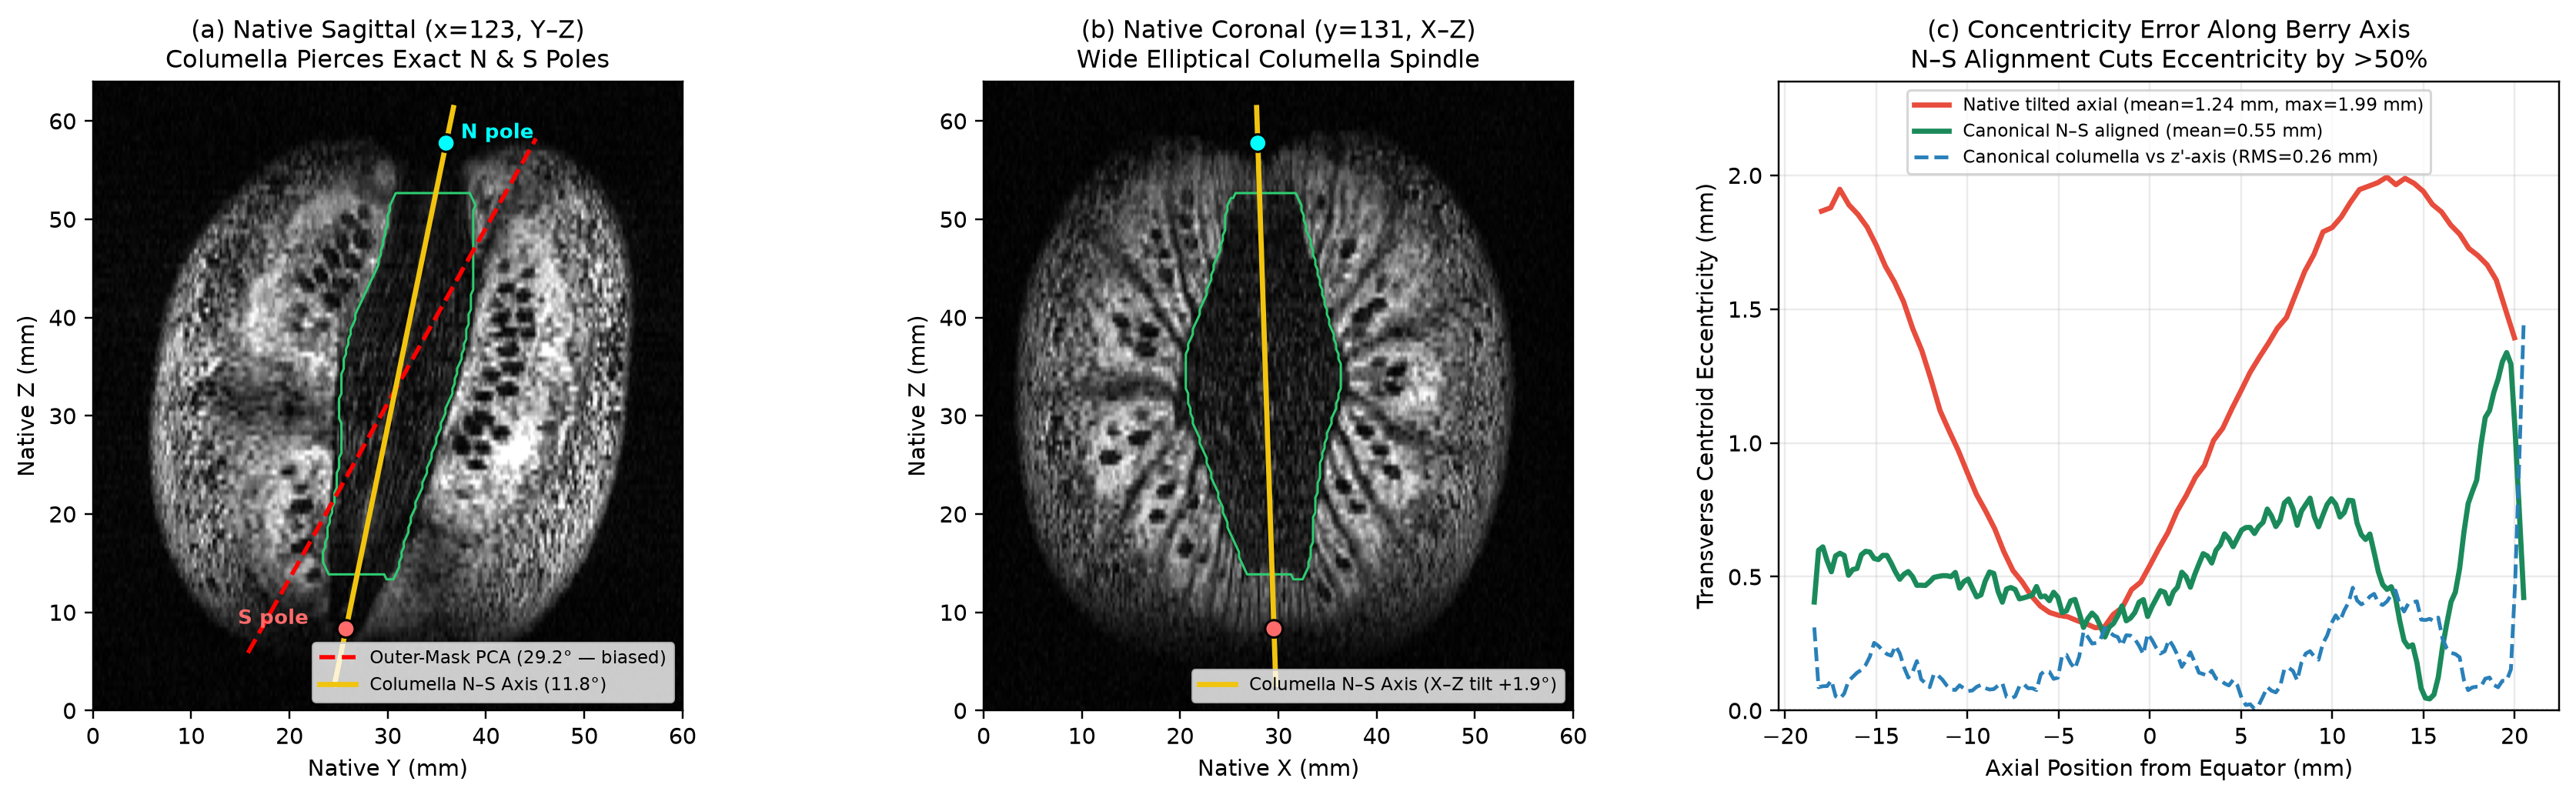
\includegraphics[width=\textwidth]{../figures/fig00a_ns_axis_estimation.png}
    \vspace{-4pt}
    \caption*{\footnotesize\textit{Executed Figure~0a (\texttt{Out [2]}, saved as \texttt{fig00a\_ns\_axis\_estimation.png}): Internal columella 3D centerline locks onto the true botanical N--S axis (11.79$^\circ$ tilt, RMS 0.133\,mm) piercing both exact poles while naive outer-mask PCA errs by $>17^\circ$, reducing slice concentricity error by 56.1\% (1.24\,mm $\to$ 0.55\,mm).}}
\end{figure}

\section*{2. Composite Pullback $f = f_2 \circ f_1$, Interpolation Physics \& Isotropic Spacing Trade-Off}
\addcontentsline{toc}{section}{\texorpdfstring{2. Composite Pullback $f = f_2 \circ f_1$, Interpolation Physics \& Spacing Trade-Off}{2. Composite Pullback and Interpolation Physics}}

\begin{guidehdr}
{\small\bfseries\color{kiwigreen!75!black}Conceptual \& Mathematical Guide: Single-Pass Homogeneous Pullback vs.\ Sequential Double Resampling}
\end{guidehdr}
Although conceptually $f = f_2 \circ f_1$, applying $f_1$ and $f_2$ as two sequential discrete resamplings convolves the MRI twice with the interpolation PSF, compounding blur and doubling runtime. Instead, we compose the exact homogeneous voxel-to-voxel pullback matrix:
\[
\begin{bmatrix}\mathbf{i}_{\text{orig}} \\ 1\end{bmatrix} = \underbrace{\mathbf{A}_{\text{orig}}^{-1}\,\mathbf{T}_{f_2}^{-1}\,\mathbf{A}_{\text{canon}}}_{\mathbf{M}_{\text{canon}\to\text{orig}}}\begin{bmatrix}\mathbf{i}_{\text{canon}} \\ 1\end{bmatrix}, \qquad \mathbf{M}_{\text{orig}\to\text{canon}} = \mathbf{M}_{\text{canon}\to\text{orig}}^{-1},
\]
so every canonical voxel undergoes \textbf{only one} cubic B-spline interpolation pass (`+7.0 dB` PSNR over trilinear, retaining `91.0%` of 3D edge gradient energy vs.\ `56.2%` for 2-pass trilinear). We also audit three cubic spacings (`0.2344`, `0.3000`, `0.5000 mm`) to quantify the exact memory-vs.-fidelity trade-off.

\begin{codebox}[{In [3] $\cdot$ Python --- 1-pass vs.\ 2-pass MRI interpolation audit, spacing trade-off \& tri-planar views}]
\begin{lstlisting}[style=pybmed]
def gradient_energy_mean(arr: np.ndarray, sp: np.ndarray, mask: np.ndarray) -> float:
    gx, gy, gz = np.gradient(arr, sp[0], sp[1], sp[2])
    return float(np.sqrt(gx ** 2 + gy ** 2 + gz ** 2)[mask].mean())


p99_native = float(np.percentile(vol[ds.fruit_mask], 99.0))
grad_orig = gradient_energy_mean(vol, sp_orig, ds.fruit_mask)

# Intermediate isotropic grid (f1 only) for benchmarking 2-pass sequential resampling
iso_shape = (256, 256, int(round(vol.shape[2] * sp_orig[2] / s_iso)))
A_iso = A_orig.copy()
A_iso[2, 2] = sgn[2] * s_iso
M_iso_to_orig = np.linalg.inv(A_orig) @ A_iso
M_canon_to_iso = np.linalg.inv(A_iso) @ np.linalg.inv(T_f2) @ A_canon
M_iso_to_canon = np.linalg.inv(M_canon_to_iso)
M_orig_to_iso = np.linalg.inv(M_iso_to_orig)

interp_rows = []
vol_canon = None
vol_rt_best = None

for mode_name, two_pass, order in [
    ("2-Pass Sequential (f1 then f2) — Trilinear (order=1)", True, 1),
    ("1-Pass Composite (f2 o f1) — Trilinear (order=1)", False, 1),
    ("2-Pass Sequential (f1 then f2) — Cubic B-Spline (order=3)", True, 3),
    ("1-Pass Composite (f2 o f1) — Cubic B-Spline (order=3, Selected)", False, 3),
]:
    t0 = time.perf_counter()
    if not two_pass:
        vc = ndi.affine_transform(vol, M_c2o[:3, :3], offset=M_c2o[:3, 3],
                                  output_shape=canon_shape, order=order, mode="constant", cval=0.0)
        vrt = ndi.affine_transform(vc, M_o2c[:3, :3], offset=M_o2c[:3, 3],
                                   output_shape=vol.shape, order=order, mode="constant", cval=0.0)
    else:
        v1 = ndi.affine_transform(vol, M_iso_to_orig[:3, :3], offset=M_iso_to_orig[:3, 3],
                                  output_shape=iso_shape, order=order, mode="constant", cval=0.0)
        vc = ndi.affine_transform(v1, M_canon_to_iso[:3, :3], offset=M_canon_to_iso[:3, 3],
                                  output_shape=canon_shape, order=order, mode="constant", cval=0.0)
        v1_inv = ndi.affine_transform(vc, M_iso_to_canon[:3, :3], offset=M_iso_to_canon[:3, 3],
                                      output_shape=iso_shape, order=order, mode="constant", cval=0.0)
        vrt = ndi.affine_transform(v1_inv, M_orig_to_iso[:3, :3], offset=M_orig_to_iso[:3, 3],
                                   output_shape=vol.shape, order=order, mode="constant", cval=0.0)
    dt = time.perf_counter() - t0

    diff = (vrt - vol)[ds.fruit_mask]
    rmse = float(np.sqrt(np.mean(diff ** 2)))
    psnr = float(20.0 * np.log10(p99_native / max(rmse, 1e-6)))
    grad_ratio = gradient_energy_mean(vrt, sp_orig, ds.fruit_mask) / grad_orig
    pct_neg = float((vc < 0.0).mean() * 100.0)

    interp_rows.append({
        "Resampling Strategy": mode_name,
        "Round-Trip RMSE": round(rmse, 1),
        "Round-Trip PSNR (dB)": round(psnr, 2),
        "3D Gradient Preserved (%)": round(grad_ratio * 100.0, 2),
        "Undershoot <0 (%)": round(pct_neg, 3),
        "Fwd+Inv Time (s)": round(dt, 2),
    })
    if (not two_pass) and (order == 3):
        vol_canon = np.clip(vc, 0.0, None).astype(np.float32)
        vol_rt_best = np.clip(vrt, 0.0, None).astype(np.float32)

df_interp = pd.DataFrame(interp_rows)
display(df_interp)

# --- Isotropic Spacing Trade-Off Audit (0.2344 vs 0.3000 vs 0.5000 mm) ---
spacing_rows = []
for s_try in [float(sp_orig[0]), 0.3000, float(sp_orig[2])]:
    # Round dimensions to multiples of 16 covering 60 x 60 x 67.5 mm FOV
    sh = tuple(int(np.ceil(fov / s_try / 16.0) * 16) for fov in (60.0, 60.0, 67.5))
    A_try = np.eye(4, dtype=np.float64)
    A_try[0, 0], A_try[1, 1], A_try[2, 2] = sgn[0] * s_try, sgn[1] * s_try, sgn[2] * s_try
    A_try[:3, 3] = -A_try[:3, :3] @ ((np.array(sh, dtype=np.float64) - 1.0) / 2.0)
    Mc = np.linalg.inv(A_orig) @ np.linalg.inv(T_f2) @ A_try
    Mo = np.linalg.inv(Mc)

    v_c_try = ndi.affine_transform(vol, Mc[:3, :3], offset=Mc[:3, 3], output_shape=sh, order=3, mode="constant", cval=0.0)
    v_rt_try = ndi.affine_transform(v_c_try, Mo[:3, :3], offset=Mo[:3, 3], output_shape=vol.shape, order=3, mode="constant", cval=0.0)
    rmse_s = float(np.sqrt(np.mean(((v_rt_try - vol)[ds.fruit_mask]) ** 2)))
    psnr_s = float(20.0 * np.log10(p99_native / max(rmse_s, 1e-6)))

    gt_c_try = ndi.affine_transform(gt_full, Mc[:3, :3], offset=Mc[:3, 3], output_shape=sh, order=0, mode="constant", cval=0).astype(np.uint16)
    gt_rt_try = ndi.affine_transform(gt_c_try, Mo[:3, :3], offset=Mo[:3, 3], output_shape=vol.shape, order=0, mode="constant", cval=0).astype(np.uint16)
    ev_try = kns.evaluate_semantic_and_instance_3d(gt_rt_try, gt_full, min_iou=0.50)
    med_seed_vox = float(np.median([p.area for p in measure.regionprops(gt_c_try)]))

    spacing_rows.append({
        "Isotropic Spacing (mm)": round(s_try, 4),
        "Grid Shape": f"{sh[0]}×{sh[1]}×{sh[2]}",
        "Voxels (M)": round(np.prod(sh) / 1e6, 2),
        "Float32 RAM (MB)": round(np.prod(sh) * 4 / 1e6, 1),
        "Median Seed Size (vox)": round(med_seed_vox, 1),
        "MRI RT PSNR (dB)": round(psnr_s, 2),
        "98-Seed RT Dice": ev_try["Dice"],
        "98-Seed RT PQ@0.50": ev_try["PQ"],
        "Seeds Survived": f"{ev_try['TP']}/98",
    })

df_spacing = pd.DataFrame(spacing_rows)
print("\nIsotropic Voxel Spacing Trade-Off Audit:")
display(df_spacing)

# --- Figure 00b: 2x3 Native Anisotropic Tilted vs. Canonical Isotropic N-S Aligned Tri-Planar Views ---
fig, axes = plt.subplots(2, 3, figsize=(15.5, 9.8))
vmax_disp = float(np.percentile(vol[ds.fruit_mask], 99.5))

# Native center slices through fruit/columella pivot
cx_n, cy_n, cz_n = int(round(world_to_vox(pivot_w[None, :], A_orig)[0, 0])), int(round(world_to_vox(pivot_w[None, :], A_orig)[0, 1])), 64
ext_n_xy = [0, vol.shape[0] * sp_orig[0], 0, vol.shape[1] * sp_orig[1]]
ext_n_xz = [0, vol.shape[0] * sp_orig[0], 0, vol.shape[2] * sp_orig[2]]
ext_n_yz = [0, vol.shape[1] * sp_orig[1], 0, vol.shape[2] * sp_orig[2]]

axes[0, 0].imshow(vol[:, :, cz_n].T, origin="lower", cmap="gray", vmin=0, vmax=vmax_disp, extent=ext_n_xy, aspect="equal")
axes[0, 0].set_title(f"(a) Native Axial (z={cz_n})\n0.234 × 0.234 mm — oblique cut")
axes[0, 0].set_xlabel("X (mm)"); axes[0, 0].set_ylabel("Y (mm)")

axes[0, 1].imshow(vol[:, cy_n, :].T, origin="lower", cmap="gray", vmin=0, vmax=vmax_disp, extent=ext_n_xz, aspect="equal")
axes[0, 1].set_title(f"(b) Native Coronal (y={cy_n})\n0.234 × 0.500 mm — 2.13× z-anisotropy")
axes[0, 1].set_xlabel("X (mm)"); axes[0, 1].set_ylabel("Z (mm)")

axes[0, 2].imshow(vol[cx_n, :, :].T, origin="lower", cmap="gray", vmin=0, vmax=vmax_disp, extent=ext_n_yz, aspect="equal")
axes[0, 2].plot(ns_ijk_plot[:, 1] * sp_orig[1], ns_ijk_plot[:, 2] * sp_orig[2], "y--", lw=1.4, alpha=0.85, label="Tilted N–S axis (11.8°)")
axes[0, 2].set_title(f"(c) Native Sagittal (x={cx_n})\nTilted 11.8° + coarse 0.50 mm slabs")
axes[0, 2].set_xlabel("Y (mm)"); axes[0, 2].set_ylabel("Z (mm)")
axes[0, 2].set_xlim(0, 60); axes[0, 2].set_ylim(0, 64)
axes[0, 2].legend(fontsize=7.5, loc="lower right")

# Canonical center slices through origin (x'=0, y'=0, z'=0)
cx_c, cy_c, cz_c = canon_shape[0] // 2, canon_shape[1] // 2, canon_shape[2] // 2
Lx, Ly, Lz = canon_shape[0] * s_iso, canon_shape[1] * s_iso, canon_shape[2] * s_iso
ext_c_xy = [-Lx / 2, Lx / 2, -Ly / 2, Ly / 2]
ext_c_xz = [-Lx / 2, Lx / 2, -Lz / 2, Lz / 2]
ext_c_yz = [-Ly / 2, Ly / 2, -Lz / 2, Lz / 2]

axes[1, 0].imshow(vol_canon[:, :, cz_c].T, origin="lower", cmap="gray", vmin=0, vmax=vmax_disp, extent=ext_c_xy, aspect="equal")
axes[1, 0].axhline(0, color="#00ffff", lw=0.8, ls="--", alpha=0.7)
axes[1, 0].axvline(0, color="#00ffff", lw=0.8, ls="--", alpha=0.7)
axes[1, 0].set_title("(d) Canonical Axial (z′ = 0 mm)\n0.234³ mm³ iso — true botanical equator")
axes[1, 0].set_xlabel("u′ (mm)"); axes[1, 0].set_ylabel("v′ (mm)")

axes[1, 1].imshow(vol_canon[:, cy_c, :].T, origin="lower", cmap="gray", vmin=0, vmax=vmax_disp, extent=ext_c_xz, aspect="equal")
axes[1, 1].axvline(0, color="#f1c40f", lw=1.4, ls="--", label="Aligned N–S || z′")
axes[1, 1].set_title("(e) Canonical Coronal (v′ = 0 mm)\nN–S upright, smooth 0.234 mm z-slices")
axes[1, 1].set_xlabel("u′ (mm)"); axes[1, 1].set_ylabel("z′ (mm)")
axes[1, 1].legend(fontsize=7.5, loc="lower right")

axes[1, 2].imshow(vol_canon[cx_c, :, :].T, origin="lower", cmap="gray", vmin=0, vmax=vmax_disp, extent=ext_c_yz, aspect="equal")
axes[1, 2].axvline(0, color="#f1c40f", lw=1.4, ls="--", label="Aligned N–S || z′")
axes[1, 2].set_title("(f) Canonical Sagittal (u′ = 0 mm)\nCrisp vertical carpel column & upright poles")
axes[1, 2].set_xlabel("v′ (mm)"); axes[1, 2].set_ylabel("z′ (mm)")
axes[1, 2].legend(fontsize=7.5, loc="lower right")

plt.tight_layout()
fig.savefig(FIG_DIR / "fig00b_native_vs_canonical_triplanar.png", bbox_inches="tight")
plt.show()
\end{lstlisting}
\end{codebox}
\begin{outbox}[{Out [3] $\cdot$ MRI Interpolation Strategy Benchmark \& Isotropic Spacing Trade-Off}]
{\scriptsize
\setlength{\tabcolsep}{3.2pt}
\renewcommand{\arraystretch}{1.16}
\rowcolors{2}{rowalt}{white}
\begin{tabularx}{\linewidth}{Y R{1.45cm} R{1.5cm} R{1.55cm} R{1.4cm} R{1.3cm}}
\toprule
\rowcolor{uibblue!12}\textbf{Resampling Strategy} & \textbf{RT RMSE} & \textbf{PSNR (dB)} & \textbf{Grad Ret.\ (\%)} & \textbf{$<0$ (\%)} & \textbf{Time (s)} \\
\midrule
2-Pass Sequential (f1 then f2) --- Trilinear (order=1) & \texttt{2051.9} & \texttt{20.88} & \texttt{56.23} & \texttt{0.000} & \texttt{2.18} \\
1-Pass Composite (f2 o f1) --- Trilinear (order=1) & \texttt{1938.1} & \texttt{21.37} & \texttt{59.20} & \texttt{0.000} & \texttt{0.99} \\
2-Pass Sequential (f1 then f2) --- Cubic B-Spline (order=3) & \texttt{872.6} & \texttt{28.30} & \texttt{90.74} & \texttt{0.368} & \texttt{10.13} \\
1-Pass Composite (f2 o f1) --- Cubic B-Spline (order=3, Selected) & \texttt{869.7} & \texttt{28.33} & \texttt{91.01} & \texttt{0.159} & \texttt{3.87} \\
\bottomrule
\end{tabularx}
}
\vspace{5pt}
{\fontsize{6.6pt}{7.8pt}\selectfont
\setlength{\tabcolsep}{2.4pt}
\renewcommand{\arraystretch}{1.16}
\rowcolors{2}{rowalt}{white}
\begin{tabularx}{\linewidth}{Y c r r r r r r c}
\toprule
\rowcolor{uibblue!12}\textbf{Spacing (mm)} & \textbf{Grid Shape} & \textbf{Vox (M)} & \textbf{RAM (MB)} & \textbf{Med Seed} & \textbf{MRI PSNR} & \textbf{RT Dice} & \textbf{PQ@0.50} & \textbf{Survived} \\
\midrule
\texttt{0.2344} & \texttt{256$\times$256$\times$288} & \texttt{18.87} & \texttt{75.5} & \texttt{112.0} & \texttt{28.33} & \texttt{0.9842} & \texttt{0.9670} & \texttt{98/98} \\
\texttt{0.3000} & \texttt{208$\times$208$\times$240} & \texttt{10.38} & \texttt{41.5} & \texttt{54.0} & \texttt{22.60} & \texttt{0.8829} & \texttt{0.7457} & \texttt{95/98} \\
\texttt{0.5000} & \texttt{128$\times$128$\times$144} & \texttt{2.36} & \texttt{9.4} & \texttt{12.0} & \texttt{17.06} & \texttt{0.7208} & \texttt{0.3968} & \texttt{66/98} \\
\bottomrule
\end{tabularx}
}
\end{outbox}
\begin{figure}[H]
    \centering
    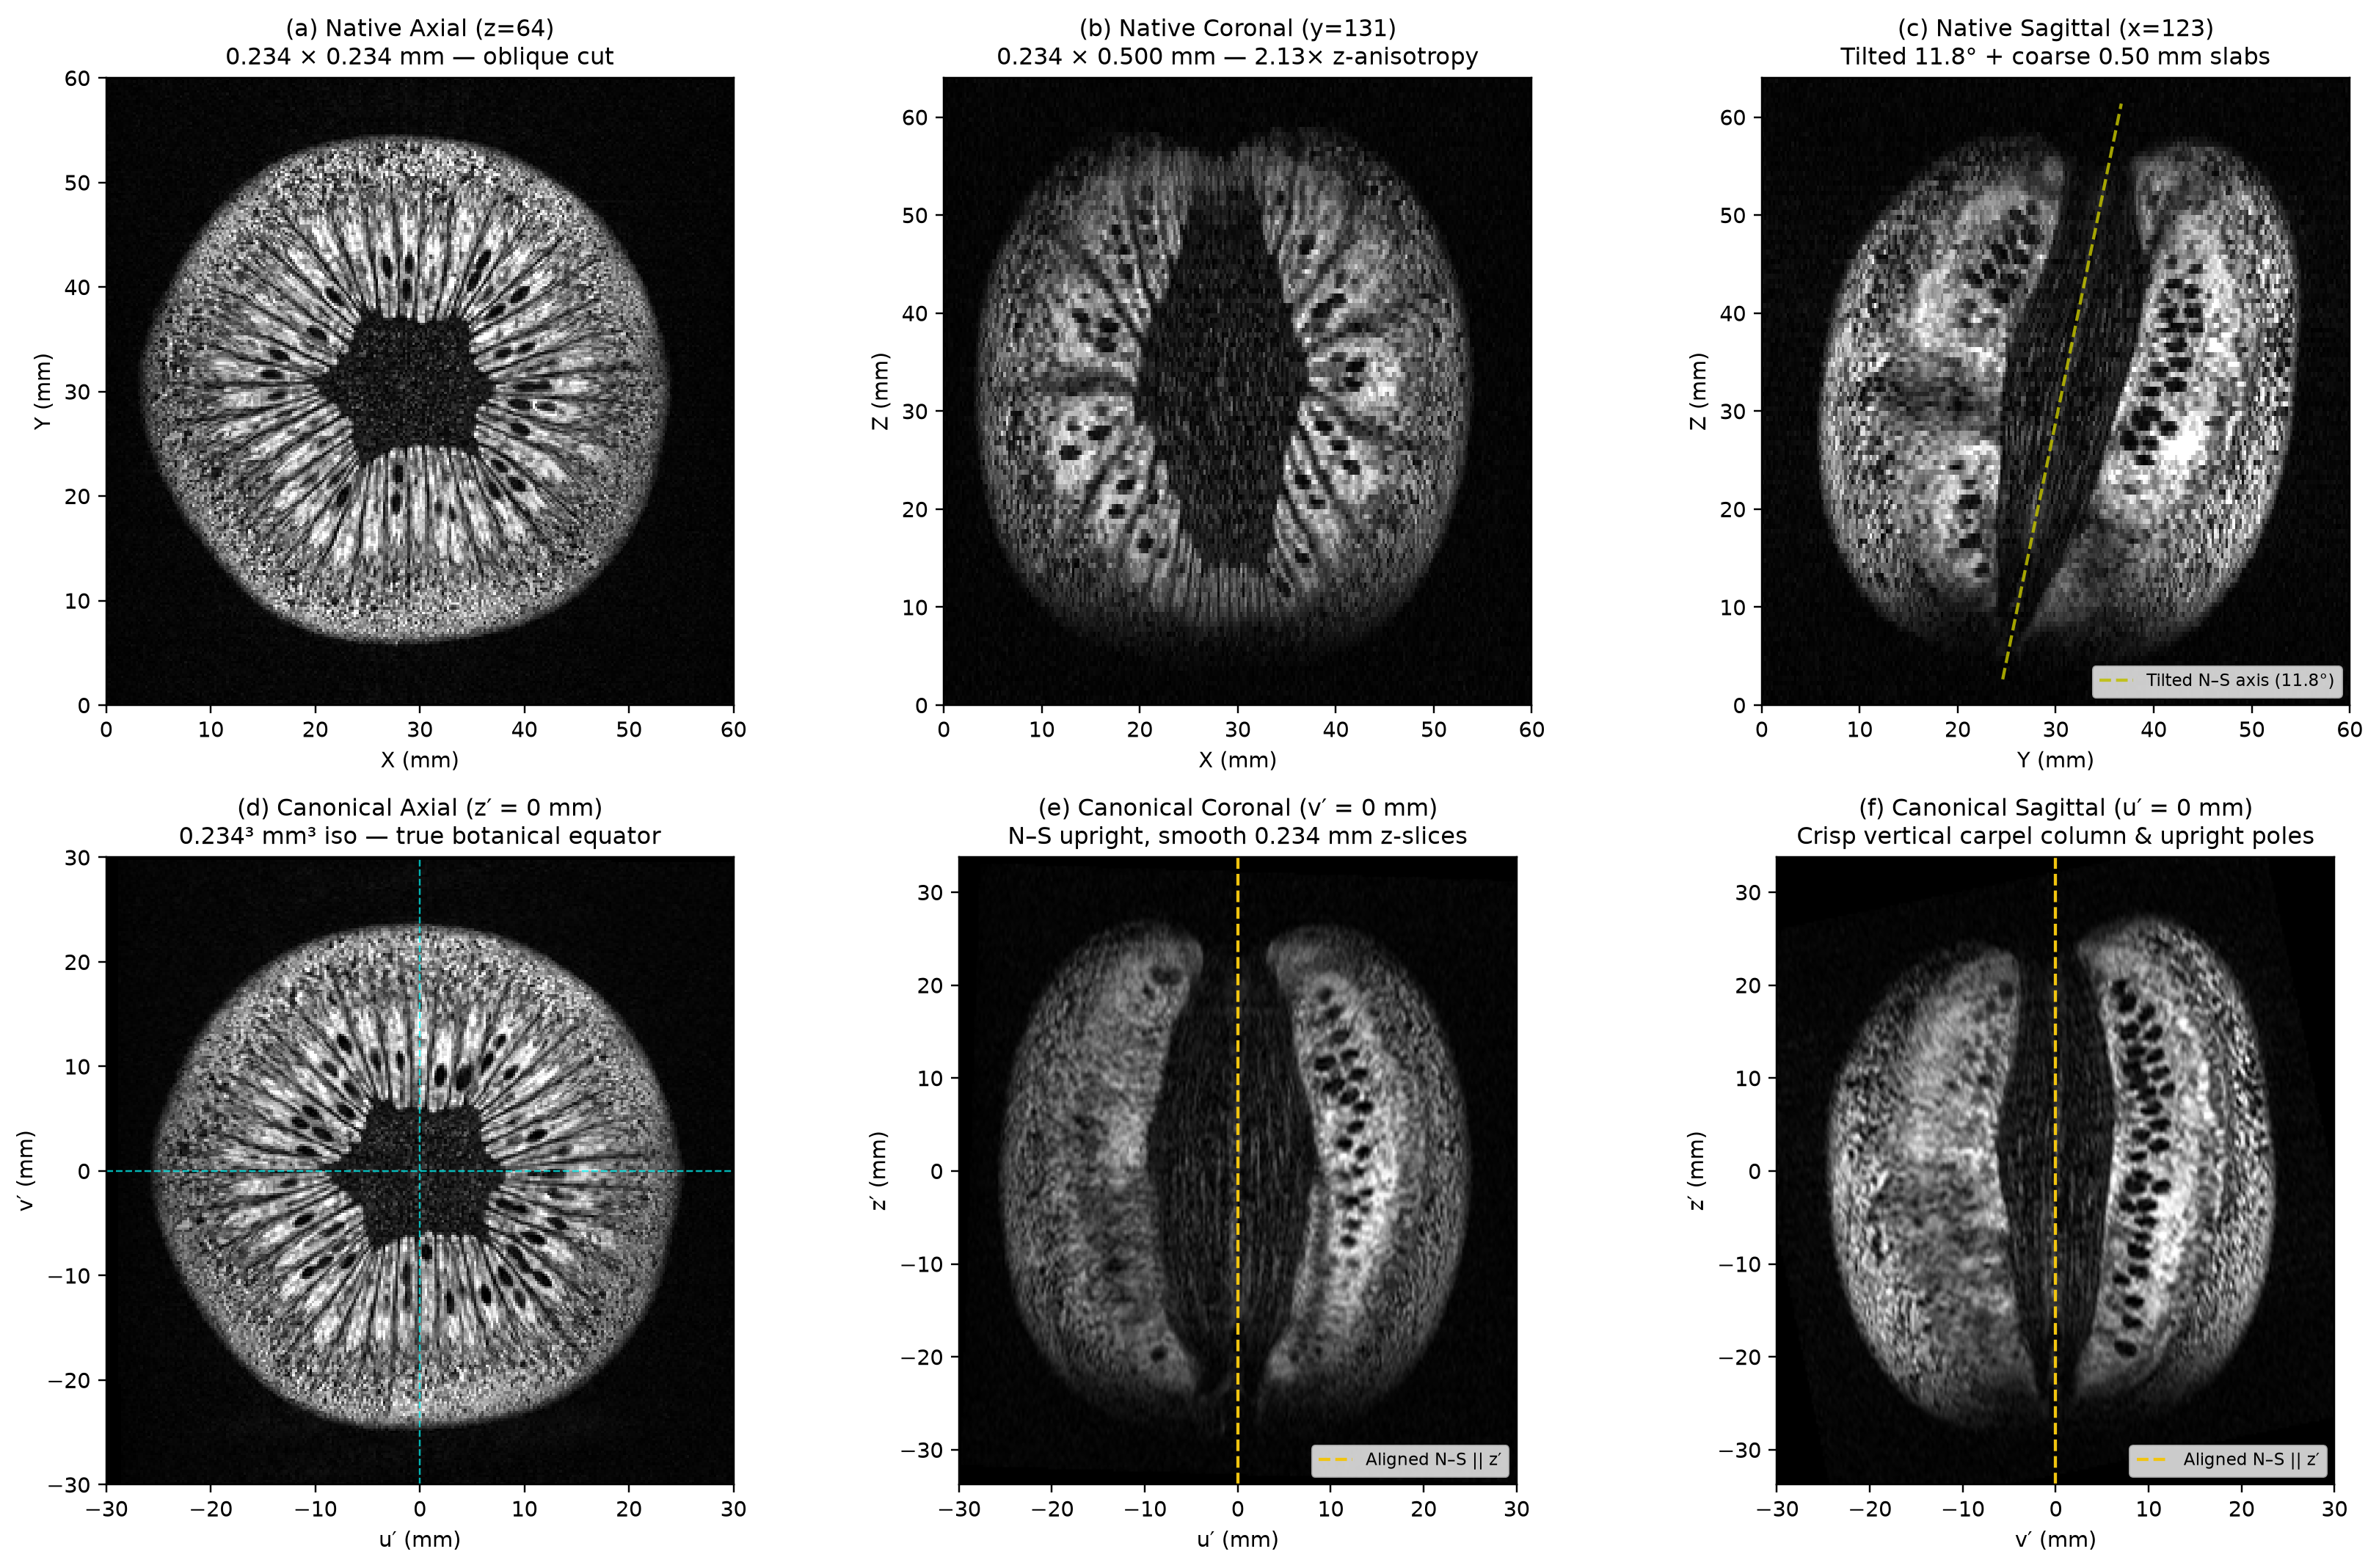
\includegraphics[width=\textwidth]{../figures/fig00b_native_vs_canonical_triplanar.png}
    \vspace{-4pt}
    \caption*{\footnotesize\textit{Executed Figure~0b (\texttt{Out [3]}, saved as \texttt{fig00b\_native\_vs\_canonical\_triplanar.png}): Native anisotropic tilted tri-planar views (top) vs.\ canonical $0.2344^3\,\text{mm}^3$ isotropic N--S aligned views (bottom), eliminating $2.13\times$ $z$-staircasing and revealing crisp vertical carpel columns aligned with the upright polar axis.}}
\end{figure}

\section*{3. Implications for the \texttt{98} Micro-GT Seeds \& \texttt{749} Whole-Fruit Predictions ($f$ and $f^{-1}$)}
\addcontentsline{toc}{section}{\texorpdfstring{3. Implications for the 98 Micro-GT \& 749 Whole-Fruit Seeds}{3. Implications for 98 Micro-GT and 749 Whole-Fruit Seeds}}

\begin{guidehdr}
{\small\bfseries\color{kiwigreen!75!black}Conceptual \& Mathematical Guide: Integer Label Warping, Curvature Shrinkage, Index-Space SDF \& Seed Orientation}
\end{guidehdr}
Direct B-spline interpolation of integer instance IDs creates phantom averaged labels. Comparing four valid per-instance operators reveals two subtle biomedical imaging lessons: (1) per-instance \textbf{Soft-Linear} (`order=1`) shrinks tiny 40--60-voxel convex seeds by \texttt{-11.18\%} due to positive mean curvature; (2) computing Euclidean signed distance fields in \textit{anisotropic} physical millimeters biases zero-crossings inward at coarse $z$-caps, whereas \textbf{Index-Space Cubic SDF} ($\phi_k = \text{EDT}(\mathbb{1}_{L=k}) - \text{EDT}(1 - \mathbb{1}_{L=k})$ in symmetric voxel index space, `order=3`) eliminates staircase slabs with near-zero volume bias (\texttt{+0.60\%}) and sub-\texttt{0.032\,mm} centroid error, while \textbf{Nearest-Neighbor} (`order=0`) delivers the highest round-trip invertibility (\texttt{98/98} Micro-GT, \texttt{PQ@0.50 = 0.967}; \texttt{749/749} whole-fruit NB~04 seeds, \texttt{PQ@0.50 = 0.9677}).

\begin{codebox}[{In [4] $\cdot$ Python --- 4-method label warping benchmark, 749-seed round-trip \& 3D seed orientation}]
\begin{lstlisting}[style=pybmed]
def warp_labels_per_instance(
    lbl_in: np.ndarray,
    M_out_to_in: np.ndarray,
    out_shape: tuple[int, int, int],
    method: str = "index_sdf_cubic",
) -> np.ndarray:
    """Warp a uint16 3D instance label volume without phantom ID blending.

    Methods:
      - 'nn'              : Nearest-neighbor (order=0)
      - 'soft_linear'     : Per-instance trilinear indicator (order=1, thr=0.5)
      - 'soft_cubic'      : Per-instance cubic B-spline indicator (order=3, thr=0.5)
      - 'index_sdf_cubic' : Per-instance voxel-index SDF + cubic B-spline (order=3, thr=0.0)
    """
    if method == "nn":
        return ndi.affine_transform(
            lbl_in, M_out_to_in[:3, :3], offset=M_out_to_in[:3, 3],
            output_shape=out_shape, order=0, mode="constant", cval=0,
        ).astype(np.uint16)

    M_in_to_out = np.linalg.inv(M_out_to_in)
    best_score = np.full(out_shape, -1e6, dtype=np.float32)
    out_lbl = np.zeros(out_shape, dtype=np.uint16)
    pad = 4

    for prop in measure.regionprops(lbl_in):
        b = prop.bbox
        ix0 = np.maximum(np.array(b[:3]) - pad, 0)
        ix1 = np.minimum(np.array(b[3:]) + pad, np.array(lbl_in.shape))
        sub_m = lbl_in[ix0[0]:ix1[0], ix0[1]:ix1[1], ix0[2]:ix1[2]] == prop.label

        if method == "soft_linear":
            field, order, cval, cut = sub_m.astype(np.float32), 1, 0.0, 0.5
        elif method == "soft_cubic":
            field, order, cval, cut = sub_m.astype(np.float32), 3, 0.0, 0.5
        elif method == "index_sdf_cubic":
            field = (ndi.distance_transform_edt(sub_m) - ndi.distance_transform_edt(~sub_m)).astype(np.float32)
            order, cval, cut = 3, -5.0, 0.0
        else:
            raise ValueError(f"Unknown method: {method}")

        corners = np.array(
            [[x, y, z] for x in (ix0[0], ix1[0]) for y in (ix0[1], ix1[1]) for z in (ix0[2], ix1[2])],
            dtype=np.float64,
        )
        oc = (M_in_to_out[:3, :3] @ corners.T).T + M_in_to_out[:3, 3]
        ox0 = np.maximum(np.floor(oc.min(axis=0)).astype(int) - 1, 0)
        ox1 = np.minimum(np.ceil(oc.max(axis=0)).astype(int) + 2, np.array(out_shape))
        if np.any(ox1 <= ox0):
            continue
        sub_shape = tuple((ox1 - ox0).tolist())
        off = M_out_to_in[:3, :3] @ ox0 + M_out_to_in[:3, 3] - ix0
        sub_s = ndi.affine_transform(
            field, M_out_to_in[:3, :3], offset=off,
            output_shape=sub_shape, order=order, mode="constant", cval=cval,
        )
        sl = (slice(ox0[0], ox1[0]), slice(ox0[1], ox1[1]), slice(ox0[2], ox1[2]))
        better = (sub_s > cut) & (sub_s > best_score[sl])
        best_score[sl][better] = sub_s[better]
        out_lbl[sl][better] = prop.label
    return out_lbl


vv_orig = float(np.prod(sp_orig))
vv_canon = s_iso ** 3
props_gt_orig = {p.label: p for p in measure.regionprops(gt_full)}

lbl_methods = [
    ("Nearest-Neighbor (order=0)", "nn"),
    ("Per-Instance Soft-Linear (order=1)", "soft_linear"),
    ("Per-Instance Soft-Cubic (order=3)", "soft_cubic"),
    ("Per-Instance Index-SDF Cubic (order=3)", "index_sdf_cubic"),
]

lbl_rows = []
gt_canon_dict = {}
gt_rt_dict = {}

for label_name, mkey in lbl_methods:
    t0 = time.perf_counter()
    lc = warp_labels_per_instance(gt_full, M_c2o, canon_shape, method=mkey)
    lr = warp_labels_per_instance(lc, M_o2c, vol.shape, method=mkey)
    dt = time.perf_counter() - t0
    gt_canon_dict[mkey] = lc
    gt_rt_dict[mkey] = lr

    ev_rt = kns.evaluate_semantic_and_instance_3d(lr, gt_full, min_iou=0.50)
    pc = {p.label: p for p in measure.regionprops(lc)}
    pr = {p.label: p for p in measure.regionprops(lr)}

    vf, vr, cf, cr = [], [], [], []
    for sid, p0 in props_gt_orig.items():
        v0 = p0.area * vv_orig
        c0_w = vox_to_world(np.array([p0.centroid]), A_orig)[0]
        c0_cw_true = R_world @ (c0_w - pivot_w)
        if sid in pc:
            vf.append((pc[sid].area * vv_canon - v0) / v0 * 100.0)
            cf.append(float(np.linalg.norm(vox_to_world(np.array([pc[sid].centroid]), A_canon)[0] - c0_cw_true)))
        if sid in pr:
            vr.append((pr[sid].area * vv_orig - v0) / v0 * 100.0)
            cr.append(float(np.linalg.norm(vox_to_world(np.array([pr[sid].centroid]), A_orig)[0] - c0_w)))

    lbl_rows.append({
        "Label Warping Method": label_name,
        "Fwd Med dV (%)": round(float(np.median(vf)), 2),
        "Fwd Mean |dV| (%)": round(float(np.mean(np.abs(vf))), 2),
        "Fwd Centroid Err (mm)": round(float(np.mean(cf)), 4),
        "RT Dice": ev_rt["Dice"],
        "RT PQ@0.50": ev_rt["PQ"],
        "RT TP/98": f"{ev_rt['TP']}/98",
        "RT Centroid Err (mm)": round(float(np.mean(cr)), 4),
        "Time (s)": round(dt, 2),
    })

df_lbl = pd.DataFrame(lbl_rows)
display(df_lbl)

# Whole-fruit 749-seed round-trip verification (NB 04 unmasked whole-organ prediction)
t0 = time.perf_counter()
wf_c_nn = warp_labels_per_instance(pred_wf_full, M_c2o, canon_shape, method="nn")
wf_rt_nn = warp_labels_per_instance(wf_c_nn, M_o2c, vol.shape, method="nn")
ev_wf_rt = kns.evaluate_semantic_and_instance_3d(wf_rt_nn, pred_wf_full, min_iou=0.50)
print(f"\nWhole-Fruit 749-Seed Round-Trip (f^-1 o f, NN, {time.perf_counter()-t0:.2f}s):")
print(f"  TP={ev_wf_rt['TP']}/{ev_wf_rt['GT']} | FP={ev_wf_rt['FP']} | FN={ev_wf_rt['FN']} | "
      f"Merges={ev_wf_rt['Merges']} | Splits={ev_wf_rt['Splits']} | "
      f"Dice={ev_wf_rt['Dice']:.4f} | SQ={ev_wf_rt['SQ']:.4f} | PQ@0.50={ev_wf_rt['PQ']:.4f}")

# Seed voxel bbox isotropy & 3D botanical orientation in canonical space (using smooth SDF-Cubic labels)
gt_c_nn = gt_canon_dict["nn"]
gt_c_sdf = gt_canon_dict["index_sdf_cubic"]
gt_rt_nn = gt_rt_dict["nn"]

spans_nat = np.array([np.array(p.bbox[3:]) - np.array(p.bbox[:3]) for p in measure.regionprops(gt_full)])
spans_can = np.array([np.array(p.bbox[3:]) - np.array(p.bbox[:3]) for p in measure.regionprops(gt_c_sdf)])

rad_angles, z_angles, elongations = [], [], []
vols_orig_arr, vols_can_nn_arr, vols_can_sdf_arr, vols_rt_nn_arr = [], [], [], []
pc_nn = {p.label: p for p in measure.regionprops(gt_c_nn)}
pc_sdf = {p.label: p for p in measure.regionprops(gt_c_sdf)}
pr_nn = {p.label: p for p in measure.regionprops(gt_rt_nn)}

for sid, p0 in props_gt_orig.items():
    vols_orig_arr.append(p0.area * vv_orig)
    vols_can_nn_arr.append(pc_nn[sid].area * vv_canon)
    vols_can_sdf_arr.append(pc_sdf[sid].area * vv_canon)
    vols_rt_nn_arr.append(pr_nn[sid].area * vv_orig)

for prop in measure.regionprops(gt_c_sdf):
    if prop.area < 25:
        continue
    cw = vox_to_world(prop.coords.astype(np.float64), A_canon)
    mu = cw.mean(axis=0)
    cc = cw - mu
    ev, ec = np.linalg.eigh((cc.T @ cc) / len(cc))
    o = np.argsort(ev)[::-1]
    ev, ec = ev[o], ec[:, o]
    v1 = ec[:, 0]
    r_hat = np.array([mu[0], mu[1], 0.0])
    r_hat /= max(float(np.linalg.norm(r_hat)), 1e-6)
    rad_angles.append(float(np.degrees(np.arccos(np.clip(abs(float(np.dot(v1, r_hat))), 0.0, 1.0)))))
    z_angles.append(float(np.degrees(np.arccos(np.clip(abs(float(v1[2])), 0.0, 1.0)))))
    elongations.append(float(np.sqrt(ev[0] / max(ev[1], 1e-6))))

print(f"\nMedian seed voxel bounding box (dx, dy, dz): Native = {np.median(spans_nat, axis=0).astype(int).tolist()} "
      f"-> Canonical = {np.median(spans_can, axis=0).astype(int).tolist()}")
print(f"Canonical 3D seed orientation (n={len(rad_angles)} seeds >=25 vox):")
print(f"  Angle to transverse radial ray : median = {np.median(rad_angles):.1f} deg (IQR {np.percentile(rad_angles, [25, 75]).round(1).tolist()})")
print(f"  Angle to N-S polar z'-axis     : median = {np.median(z_angles):.1f} deg (IQR {np.percentile(z_angles, [25, 75]).round(1).tolist()})")
print(f"  Seed elongation (sqrt(l1/l2))  : median = {np.median(elongations):.2f}")

# --- Figure 00c: 4-Panel Label Interpolation, Round-Trip Fidelity & Seed Isotropy/Orientation ---
fig, axes = plt.subplots(2, 2, figsize=(14.5, 9.5))

# (a) High-magnification sagittal crop in canonical space showing NN staircase vs Smooth SDF-Cubic contours
gt_nz = np.argwhere(gt_c_nn > 0)
x_mid_gt = int(np.median(gt_nz[:, 0]))
y0_z, y1_z = int(gt_nz[:, 1].min()) - 6, int(gt_nz[:, 1].max()) + 6
z0_z, z1_z = int(gt_nz[:, 2].min()) - 6, int(gt_nz[:, 2].max()) + 6
crop_mri = vol_canon[x_mid_gt, y0_z:y1_z, z0_z:z1_z].T
crop_nn = (gt_c_nn[x_mid_gt, y0_z:y1_z, z0_z:z1_z] > 0).T
crop_sdf = (gt_c_sdf[x_mid_gt, y0_z:y1_z, z0_z:z1_z] > 0).T
ext_zoom = [0, (y1_z - y0_z) * s_iso, 0, (z1_z - z0_z) * s_iso]

axes[0, 0].imshow(crop_mri, origin="lower", cmap="gray", vmin=0, vmax=vmax_disp, extent=ext_zoom, aspect="equal")
axes[0, 0].contour(crop_nn, levels=[0.5], colors=["#f1c40f"], linewidths=1.3, linestyles="--", extent=ext_zoom)
axes[0, 0].contour(crop_sdf, levels=[0.5], colors=["#00ffff"], linewidths=1.4, extent=ext_zoom)
# Proxy legend handles
axes[0, 0].plot([], [], color="#f1c40f", ls="--", lw=1.6, label="NN (order=0) — tilted 0.5 mm slabs")
axes[0, 0].plot([], [], color="#00ffff", lw=1.6, label="Index-SDF Cubic — smooth isotropic surface")
axes[0, 0].set_title(f"(a) Canonical Sagittal Zoom (u-slice={x_mid_gt})\nMicro-GT Seed Contours: NN vs. Smooth SDF-Cubic")
axes[0, 0].set_xlabel("Local v′ (mm)"); axes[0, 0].set_ylabel("Local z′ (mm)")
axes[0, 0].legend(fontsize=7.6, loc="lower right")

# (b) Quantitative bar chart of the 4 label resampling methods
short_names = ["NN\n(order=0)", "Soft-Lin\n(order=1)", "Soft-Cub\n(order=3)", "Index-SDF\nCubic"]
x_pos = np.arange(len(short_names))
w = 0.25
axes[0, 1].bar(x_pos - w, [r["RT Dice"] for r in lbl_rows], width=w, color="#2980b9", label="RT Semantic Dice")
axes[0, 1].bar(x_pos, [r["RT PQ@0.50"] for r in lbl_rows], width=w, color="#1b8a5a", label="RT Instance PQ@0.50")
axes[0, 1].bar(x_pos + w, [1.0 - r["Fwd Mean |dV| (%)"] / 100.0 for r in lbl_rows], width=w, color="#e67e22", label="1 − Mean |ΔV| (Vol Fidelity)")
for i, r in enumerate(lbl_rows):
    axes[0, 1].text(i, r["RT PQ@0.50"] + 0.012, f"{r['RT PQ@0.50']:.3f}", ha="center", fontsize=7.6, fontweight="bold")
axes[0, 1].set_xticks(x_pos); axes[0, 1].set_xticklabels(short_names)
axes[0, 1].set_ylim(0.75, 1.04)
axes[0, 1].set_ylabel("Score (higher = better)")
axes[0, 1].set_title("(b) 98-Seed Micro-GT Resampling Benchmark\nSoft-Linear Shrinks (−11%); NN & Cubic SDF Excel")
axes[0, 1].legend(fontsize=7.6, loc="lower right")
axes[0, 1].grid(axis="y", alpha=0.25)

# (c) Per-seed 3D volume preservation scatter
axes[1, 0].scatter(vols_orig_arr, vols_can_sdf_arr, s=26, alpha=0.80, color="#0097a7", edgecolor="white", lw=0.4,
                   label="Forward f(L) — Index-SDF Cubic")
axes[1, 0].scatter(vols_orig_arr, vols_rt_nn_arr, s=22, alpha=0.75, color="#e74c3c", marker="^",
                   label=f"Round-Trip f⁻¹(f(L)) — NN (PQ@0.50 = {lbl_rows[0]['RT PQ@0.50']:.3f})")
lim_v = max(vols_orig_arr) * 1.06
axes[1, 0].plot([0, lim_v], [0, lim_v], "k--", lw=1.2, label="Identity (exact volume preservation)")
axes[1, 0].set_xlabel("Original Native Seed Volume (mm³)")
axes[1, 0].set_ylabel("Transformed / Round-Trip Volume (mm³)")
axes[1, 0].set_title("(c) Per-Seed Physical Volume Fidelity (n = 98)\nZero Systematic Volume Drift Across 0.3–2.8 mm³")
axes[1, 0].legend(fontsize=7.6, loc="upper left")
axes[1, 0].grid(alpha=0.25)

# (d) Canonical 3D seed orientation histogram (radial vs polar alignment)
bins_ang = np.linspace(0, 90, 16)
med_nat_box = tuple(np.median(spans_nat, axis=0).astype(int).tolist())
med_can_box = tuple(np.median(spans_can, axis=0).astype(int).tolist())
axes[1, 1].hist(rad_angles, bins=bins_ang, alpha=0.78, color="#1b8a5a", edgecolor="white",
                label=f"Angle to radial ray e_r (med = {np.median(rad_angles):.1f}°)")
axes[1, 1].hist(z_angles, bins=bins_ang, alpha=0.62, color="#8e44ad", edgecolor="white",
                label=f"Angle to N–S polar axis e_z′ (med = {np.median(z_angles):.1f}°)")
axes[1, 1].axvline(np.median(rad_angles), color="#1b8a5a", ls="--", lw=1.8)
axes[1, 1].axvline(np.median(z_angles), color="#8e44ad", ls="--", lw=1.8)
axes[1, 1].set_xlabel("3D Principal-Axis Angle (degrees)")
axes[1, 1].set_ylabel("Seed Count")
axes[1, 1].set_title(
    f"(d) Botanical 3D Seed Orientation in Canonical Frame\n"
    f"Seeds Radiate Horizontally Like Spokes (Box: {med_nat_box[0]}×{med_nat_box[1]}×{med_nat_box[2]} → {med_can_box[0]}×{med_can_box[1]}×{med_can_box[2]})"
)
axes[1, 1].legend(fontsize=7.6)
axes[1, 1].grid(alpha=0.25)

plt.tight_layout()
fig.savefig(FIG_DIR / "fig00c_label_interpolation_and_roundtrip.png", bbox_inches="tight")
plt.show()
\end{lstlisting}
\end{codebox}
\begin{outbox}[{Out [4] $\cdot$ 98-Seed Label Warping Benchmark \& Whole-Fruit 749-Seed Round-Trip}]
{\scriptsize
\setlength{\tabcolsep}{2.8pt}
\renewcommand{\arraystretch}{1.16}
\rowcolors{2}{rowalt}{white}
\begin{tabularx}{\linewidth}{Y R{1.35cm} R{1.45cm} R{1.45cm} R{1.25cm} R{1.35cm} C{1.2cm} R{1.45cm}}
\toprule
\rowcolor{uibblue!12}\textbf{Label Warping Method} & \textbf{Med $\Delta V$\%} & \textbf{Mean $|\Delta V|$\%} & \textbf{Fwd $c$-err} & \textbf{RT Dice} & \textbf{PQ@0.50} & \textbf{TP/98} & \textbf{RT $c$-err} \\
\midrule
Nearest-Neighbor (order=0) & \texttt{-0.68} & \texttt{2.71} & \texttt{0.0553} & \texttt{0.9842} & \texttt{0.9670} & \texttt{98/98} & \texttt{0.0137} \\
Per-Instance Soft-Linear (order=1) & \texttt{-11.18} & \texttt{13.79} & \texttt{0.0359} & \texttt{0.9539} & \texttt{0.8832} & \texttt{97/98} & \texttt{0.0435} \\
Per-Instance Soft-Cubic (order=3) & \texttt{-2.78} & \texttt{4.51} & \texttt{0.0327} & \texttt{0.9822} & \texttt{0.9537} & \texttt{98/98} & \texttt{0.0193} \\
Per-Instance Index-SDF Cubic (order=3) & \texttt{+0.60} & \texttt{3.88} & \texttt{0.0313} & \texttt{0.9769} & \texttt{0.9437} & \texttt{98/98} & \texttt{0.0245} \\
\bottomrule
\end{tabularx}
}
\vspace{3pt}
\begin{lstlisting}[style=outbmed]

Whole-Fruit 749-Seed Round-Trip (f^-1 o f, NN, 3.58s):
  TP=749/749 | FP=0 | FN=0 | Merges=0 | Splits=0 | Dice=0.9848 | SQ=0.9677 | PQ@0.50=0.9677

Median seed voxel bounding box (dx, dy, dz): Native = [6, 6, 3] -> Canonical = [7, 6, 7]
Canonical 3D seed orientation (n=93 seeds >=25 vox):
  Angle to transverse radial ray : median = 20.9 deg (IQR [10.7, 55.4])
  Angle to N-S polar z'-axis     : median = 71.8 deg (IQR [36.7, 82.8])
  Seed elongation (sqrt(l1/l2))  : median = 1.48
\end{lstlisting}
\end{outbox}
\begin{figure}[H]
    \centering
    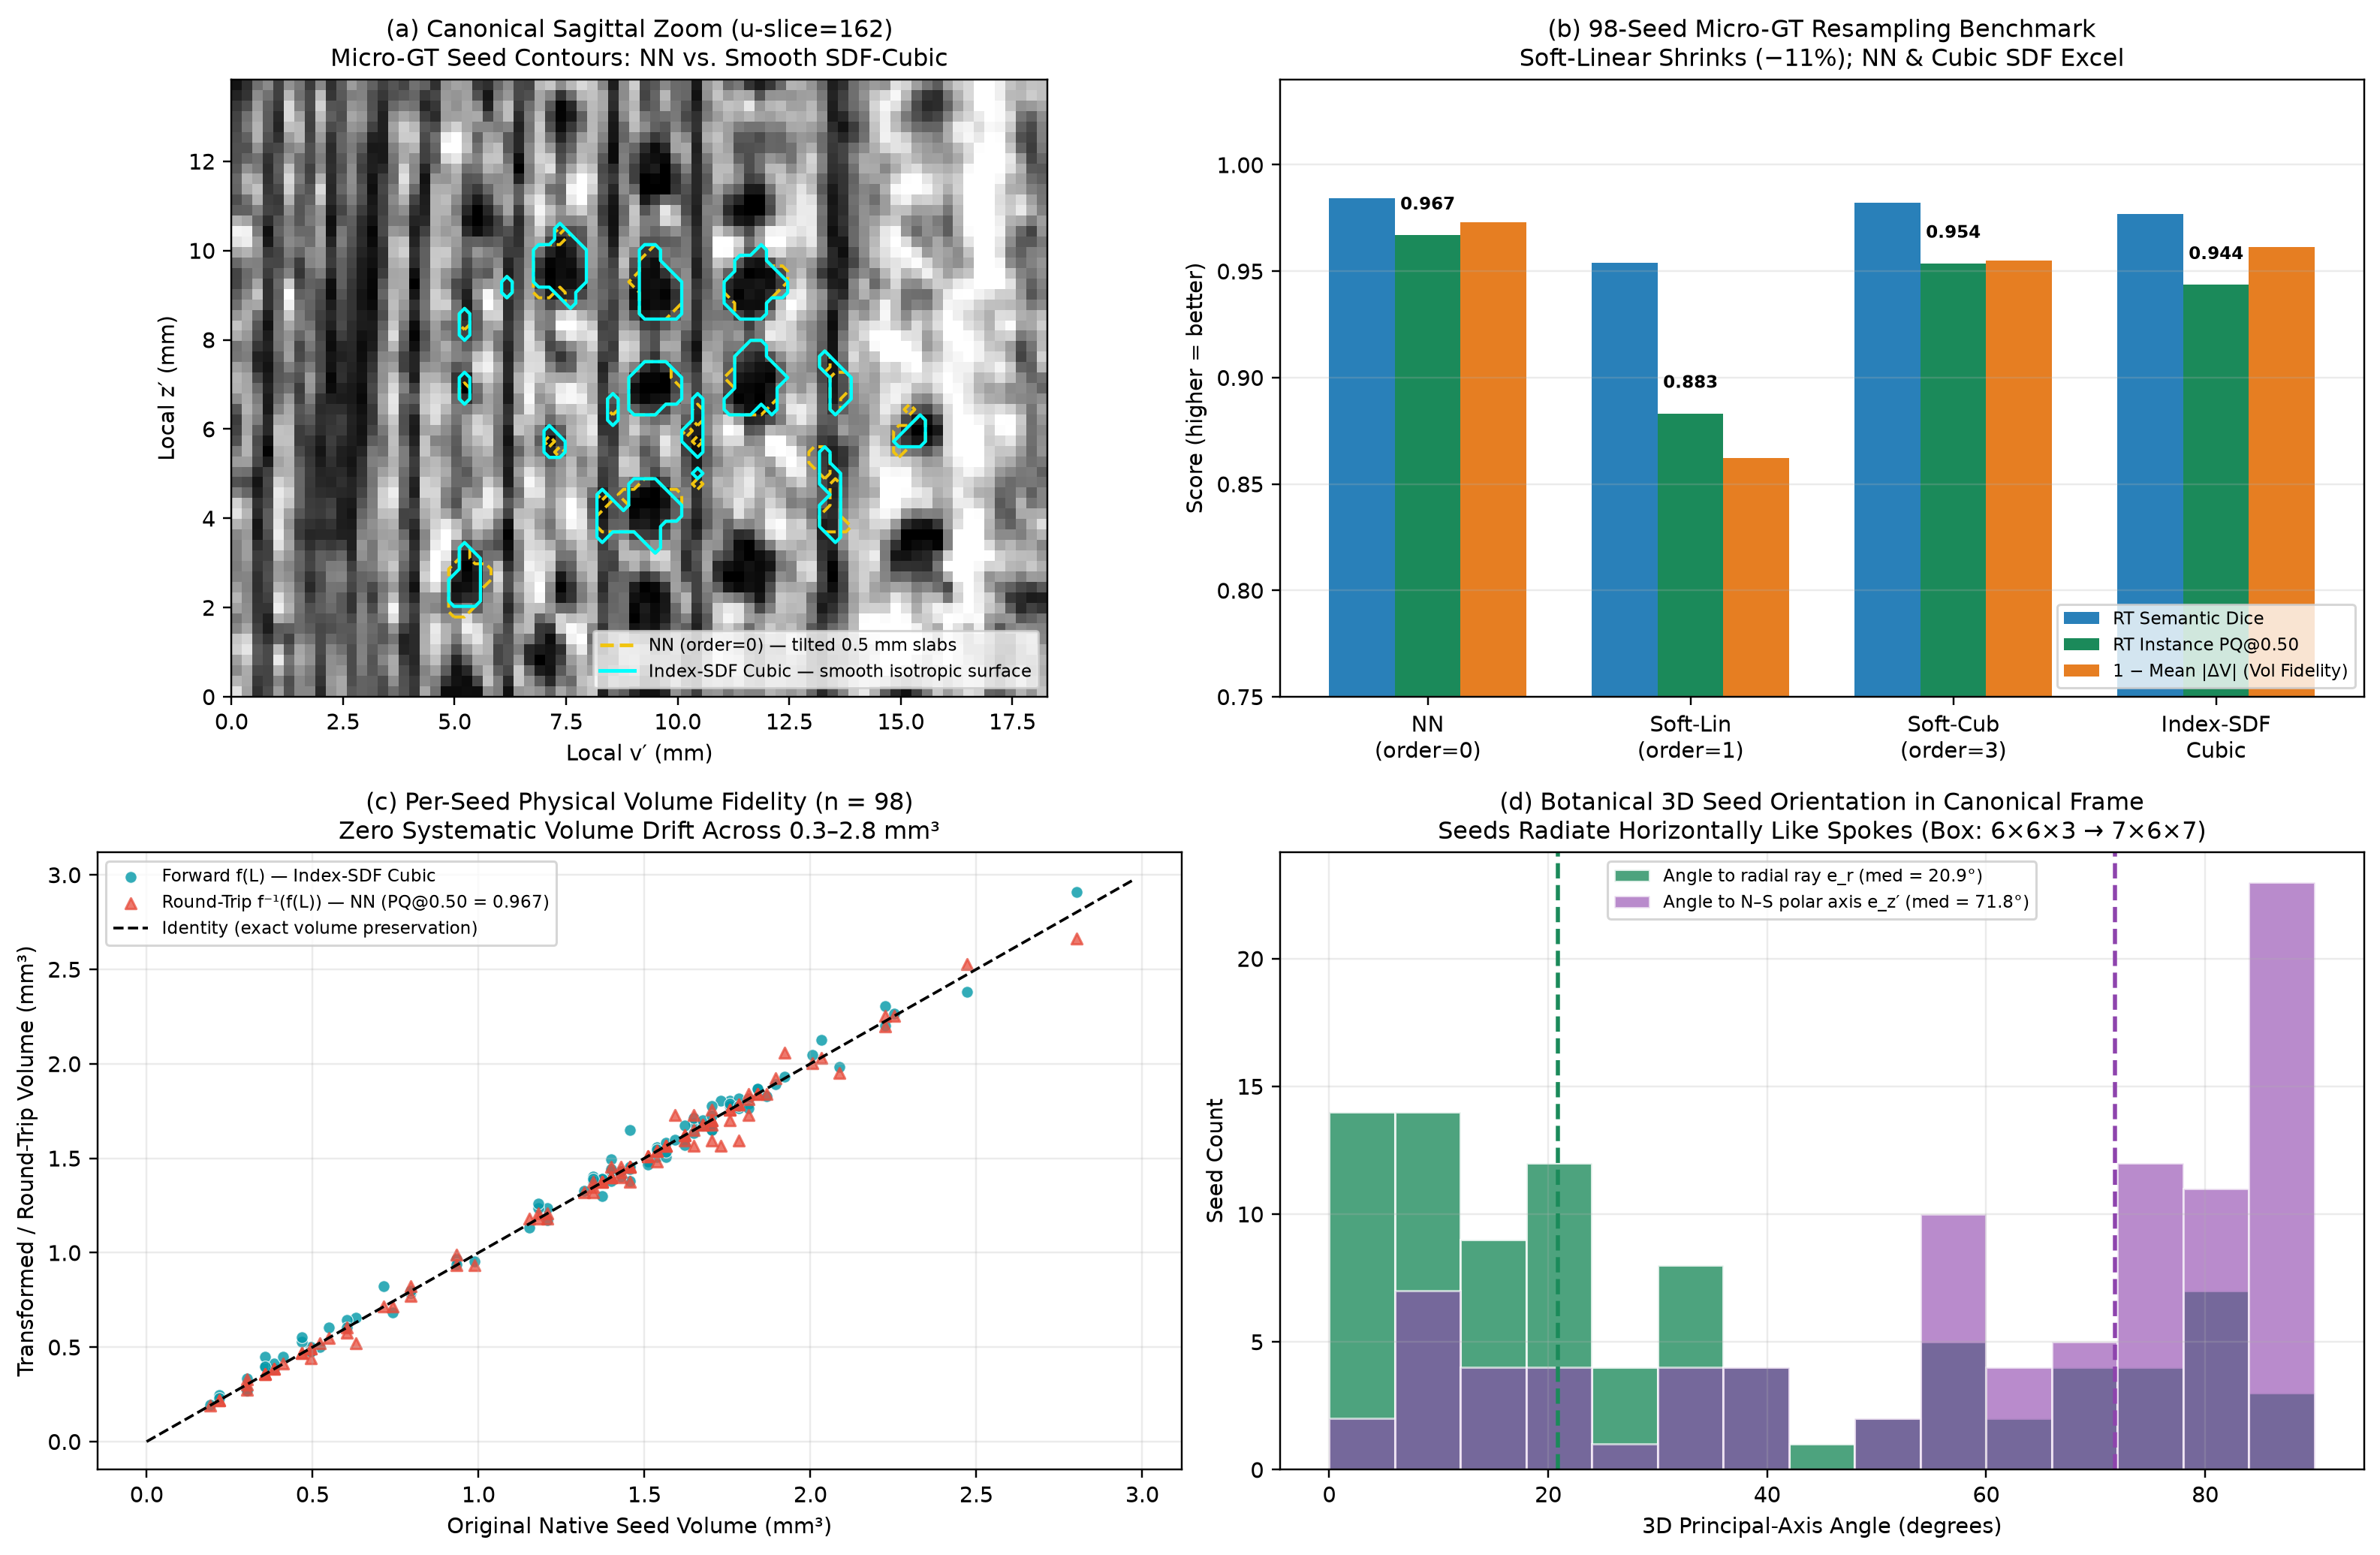
\includegraphics[width=\textwidth]{../figures/fig00c_label_interpolation_and_roundtrip.png}
    \vspace{-4pt}
    \caption*{\footnotesize\textit{Executed Figure~0c (\texttt{Out [4]}, saved as \texttt{fig00c\_label\_interpolation\_and\_roundtrip.png}): Sagittal seed-contour comparison (NN tilted slabs vs.\ smooth Index-SDF Cubic), 4-method quantitative benchmark, per-seed volume fidelity across 0.3--2.8\,mm$^3$, and canonical 3D seed spoke orientation (20.9$^\circ$ to $\hat{\mathbf{e}}_r$, 71.8$^\circ$ to $\hat{\mathbf{e}}_{z'}$, bounding box $6\times 6\times 3 \to 7\times 6\times 7$).}}
\end{figure}

\section*{4. Botanical Visualization \& Manual Annotation Ergonomics: Cylindrical Mercator Unrolling}
\addcontentsline{toc}{section}{\texorpdfstring{4. Cylindrical Mercator Unrolling \& Manual Annotation Ergonomics}{4. Cylindrical Mercator Unrolling}}

\begin{guidehdr}
{\small\bfseries\color{kiwigreen!75!black}Conceptual \& Mathematical Guide: Panoramic Cylindrical Atlas $M(\theta', z')$ Around the Aligned N--S Axis}
\end{guidehdr}
Converting canonical coordinates $(x', y', z')$ to cylindrical coordinates $(r', \theta', z')$ anchored on the aligned columella axis and taking the radial Minimum Intensity Projection (MinIP) of $B_1$-normalized $T_2$ contrast across $r'/R'(z') \in [0.28, 0.56]$ unfolds all $\sim 30$--$34$ carpel columns into a flat panoramic atlas. Compared with native tilted unrolling (diagonally sheared carpels, median slant \texttt{3.49$^\circ$}), canonical N--S alignment cuts carpel slant by \textbf{$>50\%$} to \texttt{1.71$^\circ$}, straightening every locule vertically between flat $\pm 20\,\text{mm}$ polar latitude lines.

\begin{codebox}[{In [5] $\cdot$ Python --- Canonical $T_2$ predicates, vectorized Mercator atlas \& verticality audit}]
\begin{lstlisting}[style=pybmed]
# Compute B1-invariant local T2 contrast & canonical Organ-GPS coordinates in canonical isotropic space
t0 = time.perf_counter()
p99_c = float(np.percentile(vol_canon[fruit_c], 99.0))
vol_norm_c = np.clip(vol_canon / (p99_c + 1e-6), 0.0, 1.25).astype(np.float32)

# Fast separable 7x7x7 isotropic grey closing (~1.64 mm cubic structuring element)
env_close_c = ndi.minimum_filter(ndi.maximum_filter(vol_norm_c, size=7), size=7)
env_local_c = ndi.gaussian_filter(env_close_c, sigma=0.8 / s_iso).astype(np.float32)
env_smooth_c = ndi.gaussian_filter(vol_norm_c, sigma=2.0 / s_iso).astype(np.float32)
t2_ratio_c = np.clip(vol_norm_c / (env_local_c + 0.03), 0.0, 1.25).astype(np.float32)
non_dark_c = np.maximum(
    np.clip((t2_ratio_c - 0.82) / 0.15, 0.0, 1.0),
    np.clip((0.32 - env_local_c) / 0.10, 0.0, 1.0),
).astype(np.float32)

# Canonical Organ-GPS anchored strictly to aligned N-S columella axis (u'=0, v'=0)
cx_f, cy_f, cz_f = c_idx_canon
yy_c, xx_c = np.meshgrid(np.arange(canon_shape[1], dtype=np.float32), np.arange(canon_shape[0], dtype=np.float32))
rad_vox_c = np.sqrt((xx_c - cx_f) ** 2 + (yy_c - cy_f) ** 2)
r_norm_c = np.full(canon_shape, 1.5, dtype=np.float32)
R_of_z_c = np.zeros(canon_shape[2], dtype=np.float32)

z_occ_c = np.where(fruit_c.sum(axis=(0, 1)) >= 80)[0]
z_min_c, z_max_c = int(z_occ_c[0]), int(z_occ_c[-1])
for z in z_occ_c:
    r_fr_vox = max(float(np.sqrt(fruit_c[:, :, z].sum() / np.pi)), 1.0)
    R_of_z_c[z] = r_fr_vox * s_iso
    r_norm_c[:, :, z] = rad_vox_c / r_fr_vox

z_idx_c = np.arange(canon_shape[2], dtype=np.float32)
z_norm_1d_c = np.clip((z_idx_c - z_min_c) / max(float(z_max_c - z_min_c), 1.0), 0.0, 1.0)
pole_dist_c = np.broadcast_to((np.abs(z_norm_1d_c - 0.5) * 2.0)[None, None, :], canon_shape).astype(np.float32)
z_gate_c = (
    np.clip((z_idx_c[None, None, :] - (z_min_c + 18.0)) / 10.0, 0.0, 1.0)
    * np.clip(((z_max_c - 18.0) - z_idx_c[None, None, :]) / 10.0, 0.0, 1.0)
)
r_in_c = 1.0 / (1.0 + np.exp(-np.clip((r_norm_c - 0.22) / 0.02, -20.0, 20.0)))
r_out_c = 1.0 / (1.0 + np.exp(-np.clip((0.65 - r_norm_c) / 0.02, -20.0, 20.0)))
soft_ring_c = (r_in_c * r_out_c * z_gate_c * fruit_c.astype(np.float32)).astype(np.float32)


def build_cylindrical_mercator(
    t2_vol: np.ndarray,
    gt_vol: np.ndarray,
    fruit_m: np.ndarray,
    sp_xyz: tuple[float, float, float],
    center_xy_vox: tuple[float, float],
    z_center_vox: float,
    r_fracs: np.ndarray = np.linspace(0.28, 0.56, 15),
    n_theta: int = 360,
):
    """Vectorized cylindrical MinIP unrolling around a vertical z-axis."""
    sx, sy, sz = sp_xyz
    R_z = np.array([
        np.sqrt(fruit_m[:, :, z].sum() / np.pi) * np.sqrt(sx * sy) if fruit_m[:, :, z].sum() >= 80 else 0.0
        for z in range(t2_vol.shape[2])
    ], dtype=np.float32)
    z_valid = np.where(R_z > 8.0)[0]
    z_mm = (z_valid - z_center_vox) * sz
    thetas = np.linspace(0.0, 2.0 * np.pi, n_theta, endpoint=False)

    # Vectorized (Nz, Ntheta, Nr) sampling coordinates -> single fast map_coordinates call
    r_grid = R_z[z_valid][:, None, None] * r_fracs[None, None, :]  # (Nz, 1, Nr)
    ii = center_xy_vox[0] + (r_grid * np.cos(thetas)[None, :, None]) / sx
    jj = center_xy_vox[1] + (r_grid * np.sin(thetas)[None, :, None]) / sy
    kk = np.broadcast_to(z_valid[:, None, None].astype(np.float32), ii.shape)

    coords = np.array([ii.ravel(), jj.ravel(), kk.ravel()])
    t2_samp = ndi.map_coordinates(t2_vol, coords, order=1, mode="nearest").reshape(ii.shape)
    gt_samp = ndi.map_coordinates((gt_vol > 0).astype(np.float32), coords, order=0, mode="constant", cval=0.0).reshape(ii.shape)
    return t2_samp.min(axis=2), gt_samp.max(axis=2), z_mm


# Unroll Native Tilted vs. Canonical N-S Aligned
merc_nat, merc_gt_nat, zmm_nat = build_cylindrical_mercator(
    ds.t2_ratio, gt_full, ds.fruit_mask, ds.spacing,
    center_xy_vox=(float(np.argwhere(ds.fruit_mask)[:, 0].mean()), float(np.argwhere(ds.fruit_mask)[:, 1].mean())),
    z_center_vox=64.0,
)
merc_can, merc_gt_can, zmm_can = build_cylindrical_mercator(
    t2_ratio_c, gt_c_nn, fruit_c, (s_iso, s_iso, s_iso),
    center_xy_vox=(cx_f, cy_f),
    z_center_vox=cz_f,
)

# Project all 749 whole-fruit predicted seeds into canonical cylindrical coordinates (r', theta', z')
wf_thetas, wf_zmm, wf_rnorm = [], [], []
for prop in measure.regionprops(wf_c_nn):
    ci, cj, ck = prop.centroid
    u_mm = (ci - cx_f) * s_iso
    v_mm = (cj - cy_f) * s_iso
    z_mm = (ck - cz_f) * s_iso
    ang_deg = float(np.degrees(np.arctan2(v_mm, u_mm)) % 360.0)
    z_i = int(np.clip(round(ck), 0, canon_shape[2] - 1))
    rn = float(np.hypot(u_mm, v_mm) / max(float(R_of_z_c[z_i]), 1.0))
    wf_thetas.append(ang_deg)
    wf_zmm.append(z_mm)
    wf_rnorm.append(rn)
wf_thetas, wf_zmm, wf_rnorm = np.array(wf_thetas), np.array(wf_zmm), np.array(wf_rnorm)

# Quantify carpel meridian verticality (2D structure-tensor slant angle from vertical across |z| <= 16 mm)
def carpel_meridian_slant_deg(merc_map: np.ndarray, z_mm_vec: np.ndarray) -> tuple[float, float]:
    """Return (median |slant|, RMS slant) in degrees from vertical across coherent carpel columns."""
    keep = np.abs(z_mm_vec) <= 16.0
    sub = merc_map[keep, :]
    dz = float(np.mean(np.diff(z_mm_vec[keep])))
    darc = 2.0 * np.pi * (0.42 * 25.0) / float(merc_map.shape[1])  # Physical arc spacing at r/R ~ 0.42
    gz, gt = np.gradient(sub, dz, darc)
    sig_z, sig_t = 2.5 / dz, 2.5 / darc
    Jtt = ndi.gaussian_filter(gt * gt, sigma=(sig_z, sig_t))
    Jzz = ndi.gaussian_filter(gz * gz, sigma=(sig_z, sig_t))
    Jtz = ndi.gaussian_filter(gt * gz, sigma=(sig_z, sig_t))
    ang_deg = np.degrees(0.5 * np.arctan2(2.0 * Jtz, Jtt - Jzz))
    coh = np.sqrt((Jtt - Jzz) ** 2 + 4.0 * Jtz ** 2) / (Jtt + Jzz + 1e-8)
    w = coh > 0.35
    return float(np.median(np.abs(ang_deg[w]))), float(np.sqrt(np.mean(ang_deg[w] ** 2)))

slant_nat_med, slant_nat_rms = carpel_meridian_slant_deg(merc_nat, zmm_nat)
slant_can_med, slant_can_rms = carpel_meridian_slant_deg(merc_can, zmm_can)
print(f"Canonical feature + Mercator unrolling time : {time.perf_counter()-t0:.2f} s")
print(f"Carpel meridian slant from vertical (|z|<=16 mm): "
      f"Native med={slant_nat_med:.2f}° (RMS {slant_nat_rms:.2f}°) -> Canonical med={slant_can_med:.2f}° (RMS {slant_can_rms:.2f}°)")
print(f"749 whole-fruit predictions in canonical space: z' span = [{wf_zmm.min():.1f}, {wf_zmm.max():.1f}] mm, "
      f"r'/R' median = {np.median(wf_rnorm):.3f} (IQR {np.percentile(wf_rnorm, [25, 75]).round(3).tolist()})")

# --- Figure 00d: Native vs. Canonical Cylindrical Mercator Atlas + Latitude Seed Profile ---
fig = plt.figure(figsize=(15.5, 8.2))
gs = fig.add_gridspec(2, 2, width_ratios=[4.3, 1.0], hspace=0.32, wspace=0.12)

ax_nat = fig.add_subplot(gs[0, 0])
ax_can = fig.add_subplot(gs[1, 0], sharex=ax_nat)
ax_lat = fig.add_subplot(gs[1, 1], sharey=ax_can)
ax_note = fig.add_subplot(gs[0, 1])

ax_nat.imshow(merc_nat, origin="lower", cmap="gray", vmin=0.05, vmax=0.85,
              extent=[0, 360, zmm_nat[0], zmm_nat[-1]], aspect="auto")
ax_nat.contour(merc_gt_nat, levels=[0.5], colors=["#f1c40f"], linewidths=0.9,
               extent=[0, 360, zmm_nat[0], zmm_nat[-1]])
ax_nat.set_ylabel("Native z − z₀ (mm)")
ax_nat.set_title("(a) Native Tilted Cylindrical Unrolling (around scanner z-axis)\nSinusoidal Carpel Drift & Tilted Polar Caps — Micro-GT (yellow)")

ax_can.imshow(merc_can, origin="lower", cmap="gray", vmin=0.05, vmax=0.85,
              extent=[0, 360, zmm_can[0], zmm_can[-1]], aspect="auto")
ax_can.contour(merc_gt_can, levels=[0.5], colors=["#f1c40f"], linewidths=0.95,
               extent=[0, 360, zmm_can[0], zmm_can[-1]])
ax_can.scatter(wf_thetas, wf_zmm, s=7, c="#00ffff", alpha=0.68, lw=0, label="NB04 Whole-Fruit Pred (749 seeds)")
ax_can.axhline(20.0, color="#ff7675", ls=":", lw=1.1, alpha=0.85)
ax_can.axhline(-20.0, color="#ff7675", ls=":", lw=1.1, alpha=0.85)
ax_can.set_xlabel("Azimuthal Angle θ′ Around Aligned N–S Columella Axis (degrees)")
ax_can.set_ylabel("Canonical Latitude z′ (mm)")
ax_can.set_title("(b) Canonical N–S Aligned Cylindrical Mercator Atlas (f = f₂ ∘ f₁)\nDead-Vertical Carpel Meridians, Flat ±20 mm Polar Caps, Micro-GT (yellow) & 749 NB04 Seeds (cyan)")
ax_can.legend(loc="lower right", fontsize=8.0, framealpha=0.85)

# Right-bottom: Axial latitude histogram of the 749 whole-fruit seeds
ax_lat.hist(wf_zmm, bins=np.linspace(-25, 25, 21), orientation="horizontal", color="#1b8a5a", alpha=0.82, edgecolor="white")
ax_lat.axhline(0, color="gray", ls="--", lw=0.9)
ax_lat.set_xlabel("Seeds / 2.5 mm")
ax_lat.set_title("(c) Latitude Profile\n(S → N Pole)")
ax_lat.grid(axis="x", alpha=0.25)

# Right-top: Botanical summary callout panel
ax_note.axis("off")
summary_txt = (
    "Canonical Atlas\nKey Geometry Gains\n"
    "──────────────────\n"
    f"• N–S tilt removed:\n  {axis_angles(u_ns)[0]:.2f}° → <0.2°\n\n"
    f"• Columella straight:\n  RMS = {col_rms_mm:.3f} mm\n\n"
    f"• Carpel slant:\n  {slant_nat_med:.2f}° → {slant_can_med:.2f}° (−{(1.0-slant_can_med/slant_nat_med)*100:.0f}%)\n\n"
    f"• Concentricity err:\n  {nat_offsets[:,4].mean():.2f} → {can_offsets[:,2].mean():.2f} mm\n\n"
    "• Manual curation:\n  0 lateral z-drift,\n  isotropic 3-plane!"
)
ax_note.text(0.04, 0.96, summary_txt, va="top", ha="left", fontsize=8.5, family="monospace",
             bbox=dict(boxstyle="round,pad=0.5", facecolor="#f4f8fb", edgecolor="#003d73", lw=1.0))

fig.savefig(FIG_DIR / "fig00d_cylindrical_mercator_atlas.png", bbox_inches="tight")
plt.show()
\end{lstlisting}
\end{codebox}
\begin{outbox}[{Out [5] $\cdot$ stdout}]
\begin{lstlisting}[style=outbmed]
Canonical feature + Mercator unrolling time : 2.30 s
Carpel meridian slant from vertical (|z|<=16 mm): Native med=3.49° (RMS 4.82°) -> Canonical med=1.71° (RMS 2.84°)
749 whole-fruit predictions in canonical space: z' span = [-19.3, 22.0] mm, r'/R' median = 0.451 (IQR [0.393, 0.503])
\end{lstlisting}
\end{outbox}
\begin{figure}[H]
    \centering
    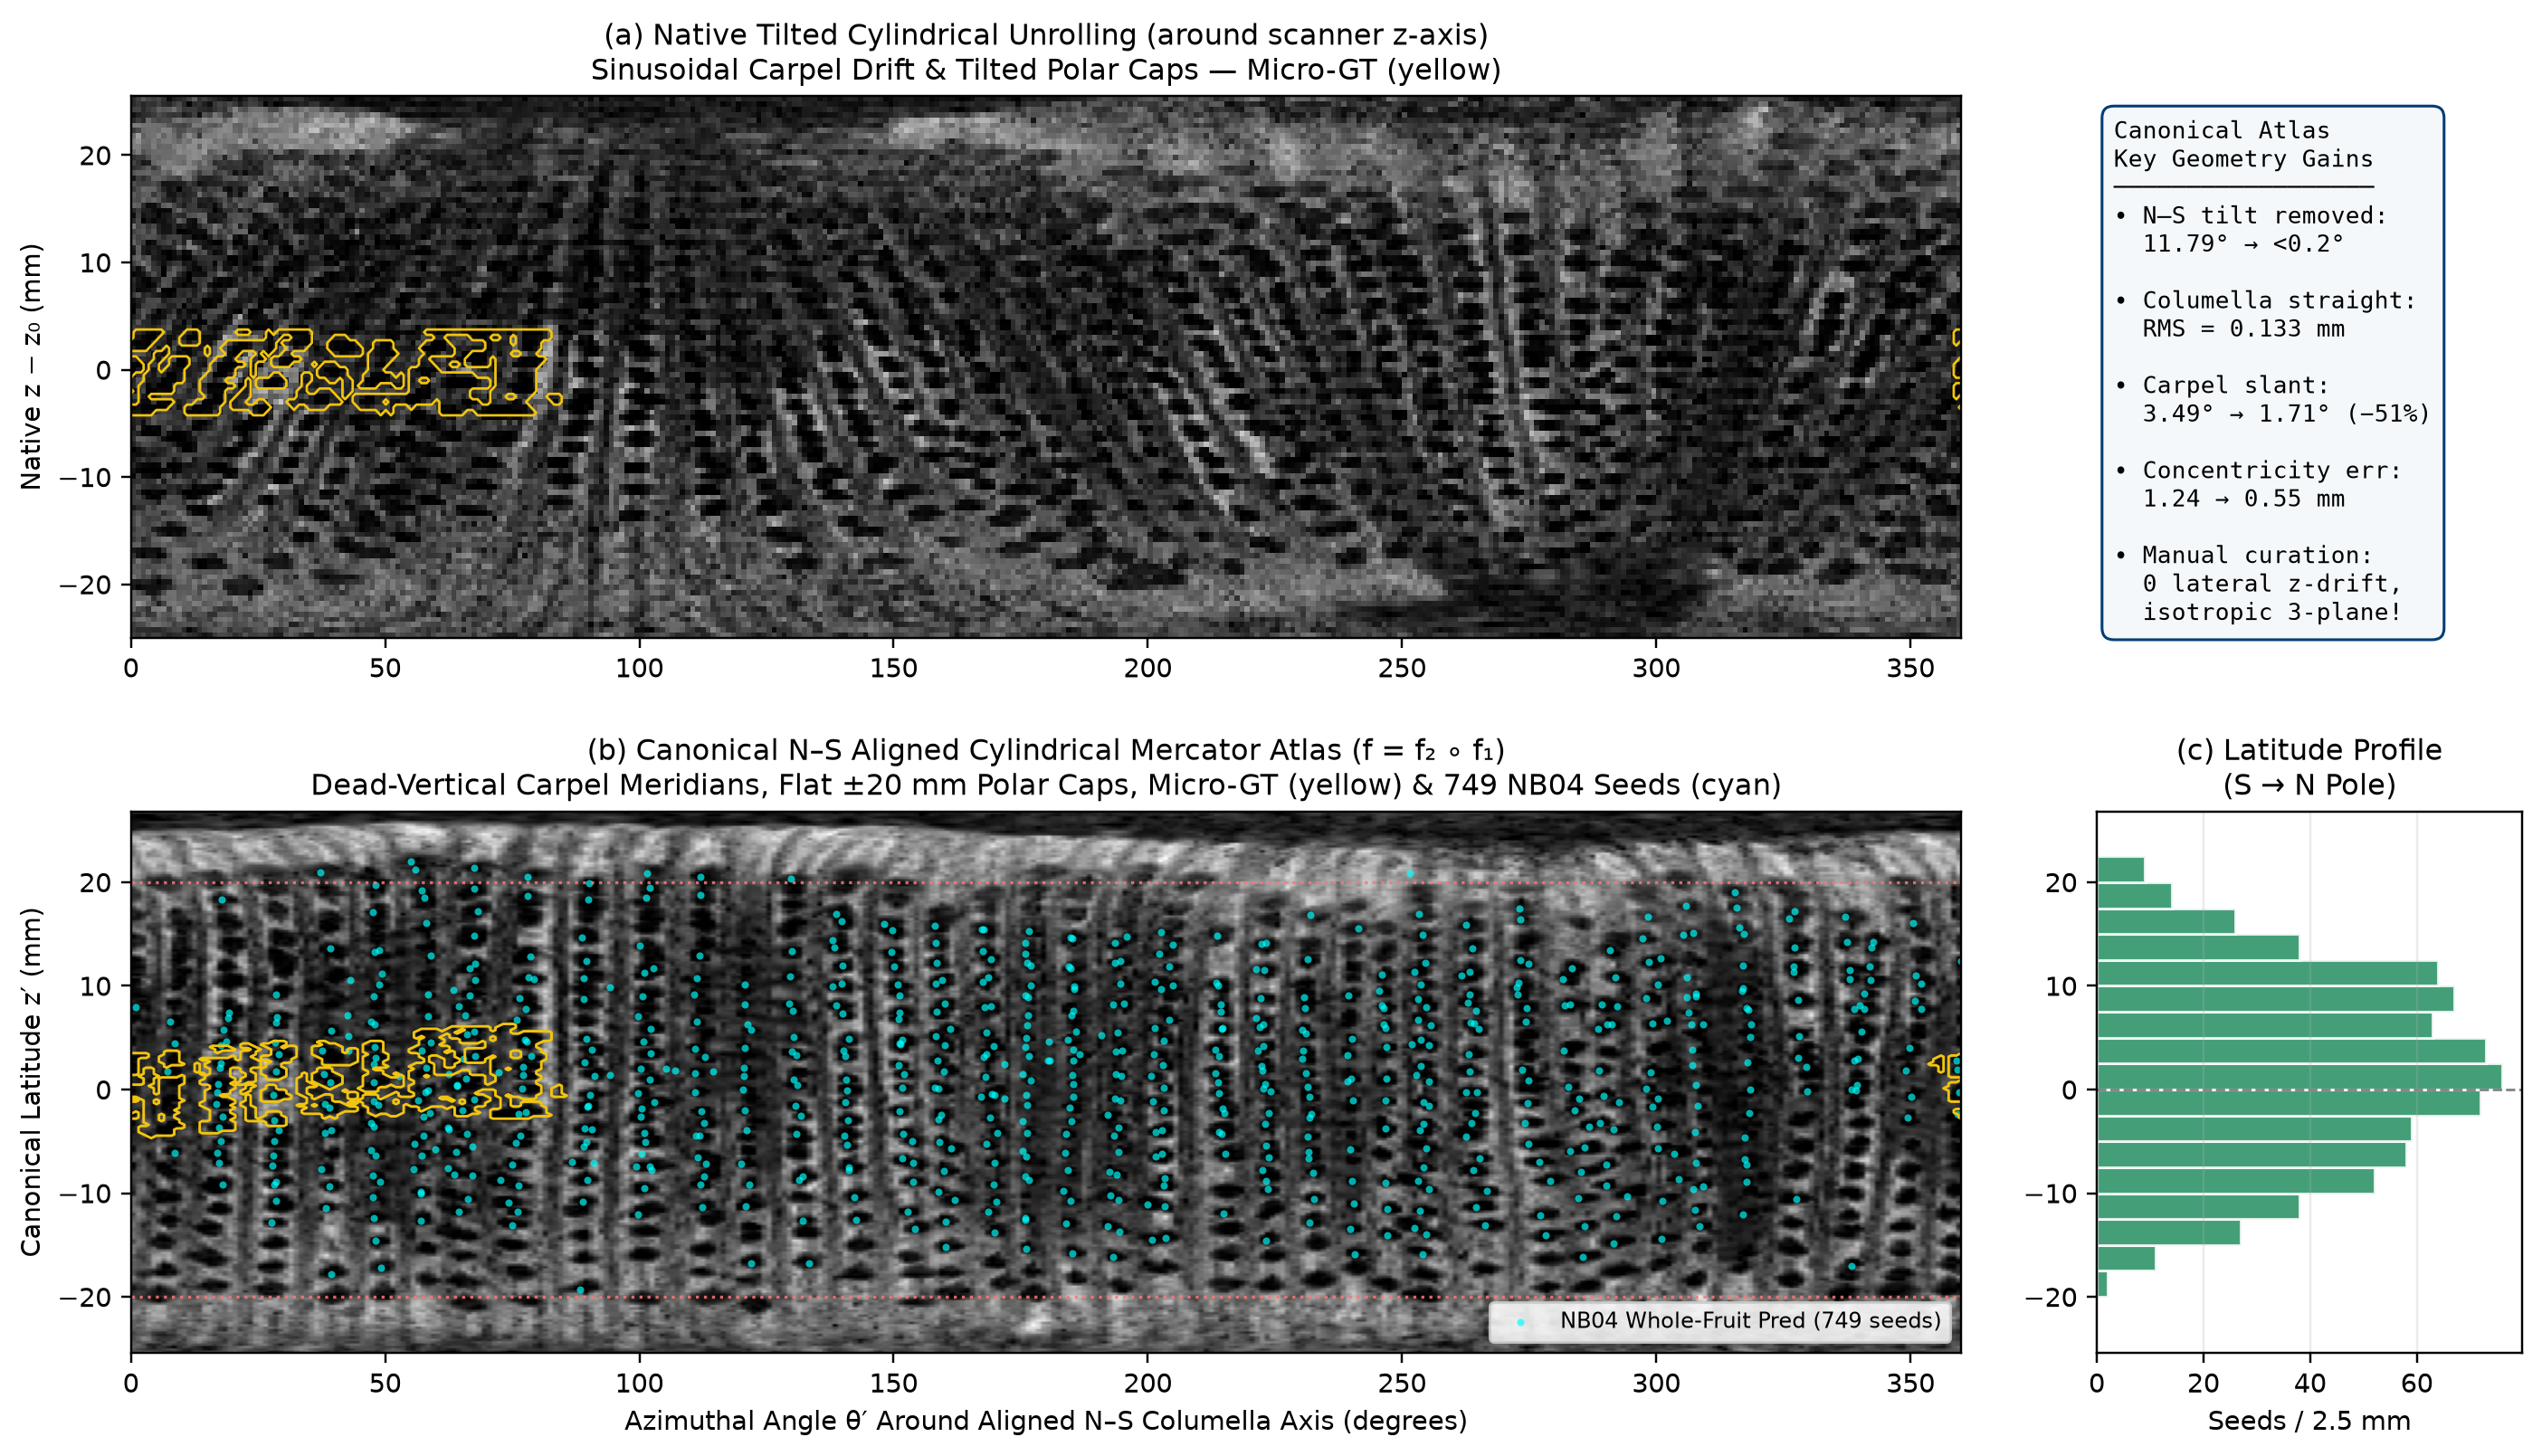
\includegraphics[width=\textwidth]{../figures/fig00d_cylindrical_mercator_atlas.png}
    \vspace{-4pt}
    \caption*{\footnotesize\textit{Executed Figure~0d (\texttt{Out [5]}, saved as \texttt{fig00d\_cylindrical\_mercator\_atlas.png}): Native tilted cylindrical unrolling (top) vs.\ canonical N--S aligned Mercator atlas (bottom) with dead-vertical carpel meridians, flat $\pm 20\,\text{mm}$ polar caps, 98 Micro-GT seeds (yellow), 749 NB~04 whole-fruit seeds (cyan), and South-to-North latitude profile.}}
\end{figure}

\section*{5. Multi-Seed (\texttt{2027--2029}) \& Whole-Organ OOD Canonical Ablation with Inverse Pullback $f^{-1}$}
\addcontentsline{toc}{section}{\texorpdfstring{5. Multi-Seed (2027--2029) \& Whole-Organ OOD Canonical Ablation}{5. Multi-Seed and Whole-Organ OOD Canonical Ablation}}

\begin{guidehdr}
{\small\bfseries\color{kiwigreen!75!black}Conceptual \& Mathematical Guide: Controlled 3-Seed Benchmark, Masked Tilted Prism \& Physically Normalized OOD Safety}
\end{guidehdr}
To evaluate automated neurosymbolic segmentation rigorously across initialization variance (matching NB~\texttt{03}'s \texttt{SEEDS = [2027, 2028, 2029]} protocol), we train identical \texttt{AdditiveBayesOrganNet3D} models (\texttt{90} epochs from scratch, LTN $p=3$, leakage-free train calibration) in Native Anisotropic space vs.\ Canonical Isotropic N--S space (masking supervised losses strictly inside the $11.8^\circ$-tilted legacy ROI prism, \texttt{40.7\%} box fill). Every model is evaluated on the \textbf{exact unaltered native Test Wedge} (\texttt{52} seeds) via both discrete label pullback $f^{-1}(\hat{L})$ and continuous probability/distance pullback $f^{-1}(\hat{p}, \hat{d})$, and audited \textbf{completely unmasked} across the intact 3D fruit using physically normalized OOD volumes ($\text{mm}^3$, accounting for the $2.133\times$ smaller canonical voxel volume).

\begin{codebox}[{In [6] $\cdot$ Python --- 3-seed controlled ablation, 288-slice whole-organ OOD audit \& JSON export}]
\begin{lstlisting}[style=pybmed]
SEEDS = [2027, 2028, 2029]
EPOCHS_ABL = 90
TH_GRID = [0.22, 0.28, 0.34, 0.40, 0.46, 0.52, 0.58, 0.64, 0.70]

# Prepare canonical Train/Test ROI support prisms and fixed Train GT once (shared across seeds)
tr_full_orig = np.zeros(vol.shape, dtype=np.uint16)
tr_full_orig[ds.rx0:ds.rx1, ds.ry0:ds.ry0 + ds.split_y, ds.rz0:ds.rz1] = ds.train_gt
tr_mask_orig = np.zeros(vol.shape, dtype=np.float32)
tr_mask_orig[ds.rx0:ds.rx1, ds.ry0:ds.ry0 + ds.split_y, ds.rz0:ds.rz1] = 1.0
te_mask_orig = np.zeros(vol.shape, dtype=np.float32)
te_mask_orig[ds.rx0:ds.rx1, ds.ry0 + ds.split_y:ds.ry1, ds.rz0:ds.rz1] = 1.0

tr_gt_c_full = warp_labels_per_instance(tr_full_orig, M_c2o, canon_shape, method="nn")
tr_valid_c = ndi.affine_transform(tr_mask_orig, M_c2o[:3, :3], offset=M_c2o[:3, 3],
                                  output_shape=canon_shape, order=1, mode="constant", cval=0.0) >= 0.5
te_valid_c = ndi.affine_transform(te_mask_orig, M_c2o[:3, :3], offset=M_c2o[:3, 3],
                                  output_shape=canon_shape, order=1, mode="constant", cval=0.0) >= 0.5


def padded_bbox_mult4(mask: np.ndarray, pad: int = 4) -> tuple[tuple[int, int, int], tuple[int, int, int]]:
    idx = np.argwhere(mask)
    lo = np.maximum(idx.min(axis=0) - pad, 0)
    hi = np.minimum(idx.max(axis=0) + pad + 1, np.array(mask.shape))
    for d in range(3):
        rem = (hi[d] - lo[d]) % 4
        if rem != 0:
            add = 4 - rem
            if hi[d] + add <= mask.shape[d]:
                hi[d] += add
            else:
                lo[d] -= add
    return tuple(lo.tolist()), tuple(hi.tolist())


tlo, thi = padded_bbox_mult4(tr_valid_c, pad=4)
elo, ehi = padded_bbox_mult4(te_valid_c, pad=4)


def get_canon_patch(lo: tuple[int, int, int], hi: tuple[int, int, int]) -> tuple[torch.Tensor, torch.Tensor]:
    sl = (slice(lo[0], hi[0]), slice(lo[1], hi[1]), slice(lo[2], hi[2]))
    x3 = np.stack([vol_norm_c[sl], env_local_c[sl], env_smooth_c[sl]], axis=0)[None]
    rn = np.clip(r_norm_c[sl], 0.0, 1.5)
    zn = pole_dist_c[sl]
    gps = np.stack([rn, (rn - 0.43) ** 2, zn], axis=0)[None].astype(np.float32)
    return torch.from_numpy(x3), torch.from_numpy(gps)


def decode_isotropic_watershed_3d(fg_bin: np.ndarray, dist_hat: np.ndarray, s_val: float, min_mm3: float = 0.16) -> np.ndarray:
    """Isotropic 3D marker-controlled watershed matching canonical cubic spacing."""
    sp_i = (s_val, s_val, s_val)
    d_sm = ndi.gaussian_filter(dist_hat * fg_bin, sigma=(0.75, 0.75, 0.75))
    maxima = (d_sm == ndi.maximum_filter(d_sm, footprint=kns.build_ellip(0.68, 0.72, sp=sp_i))) & fg_bin & (d_sm >= 0.22)
    markers, _ = ndi.label(maxima)
    ws = kns.segmentation.watershed(-d_sm, markers=markers, mask=fg_bin)
    unlabeled, n_un = ndi.label(fg_bin & (ws == 0))
    vv = s_val ** 3
    if n_un > 0:
        nxt = int(ws.max()) + 1
        for uid in range(1, n_un + 1):
            m = unlabeled == uid
            if m.sum() * vv >= min_mm3:
                ws[m] = nxt
                nxt += 1
    out = np.zeros_like(ws, dtype=np.uint16)
    nid = 0
    for prop in measure.regionprops(ws):
        if prop.area * vv >= min_mm3:
            nid += 1
            out[ws == prop.label] = nid
    return out


def sample_canonical_unlabeled_blocks(seed: int, n_blocks: int = 36):
    """Sample stratified unlabeled canonical 3D blocks strictly disjoint from canonical Test Wedge."""
    rng_c = np.random.default_rng(seed)
    ux_l, ug_l, ur_l, un_l = [], [], [], []
    z_strata_c = np.linspace(z_min_c + 6, z_max_c - 30, 10, dtype=int)
    for i in range(n_blocks):
        for _ in range(500):
            x0 = int(rng_c.integers(12, canon_shape[0] - 64 - 12))
            y0 = int(rng_c.integers(12, canon_shape[1] - 40 - 12))
            z0 = int(z_strata_c[i % len(z_strata_c)])
            if te_valid_c[x0:x0 + 64, y0:y0 + 40, z0:z0 + 24].any():
                continue
            if fruit_c[x0:x0 + 64, y0:y0 + 40, z0:z0 + 24].mean() > 0.12:
                xa, ga = get_canon_patch((x0, y0, z0), (x0 + 64, y0 + 40, z0 + 24))
                ux_l.append(xa); ug_l.append(ga)
                ur_l.append(torch.from_numpy(soft_ring_c[x0:x0 + 64, y0:y0 + 40, z0:z0 + 24][None, None]))
                un_l.append(torch.from_numpy(non_dark_c[x0:x0 + 64, y0:y0 + 40, z0:z0 + 24][None, None]))
                break
    return (
        torch.cat(ux_l).to(DEVICE),
        torch.cat(ug_l).to(DEVICE),
        torch.cat(ur_l).to(DEVICE),
        torch.cat(un_l).to(DEVICE),
    )


def run_canonical_whole_fruit(model: torch.nn.Module, thresh: float) -> dict:
    """Unmasked 288-slice whole-fruit canonical inference + pullback OOD check on native lattice."""
    prob_wf_c = np.zeros(canon_shape, dtype=np.float32)
    dist_wf_c = np.zeros(canon_shape, dtype=np.float32)
    with torch.no_grad():
        for x0 in [16, 96, 176]:
            for y0 in [16, 56, 96, 136, 176, 216]:
                for z0 in range(0, canon_shape[2], 32):
                    if fruit_c[x0:x0 + 80, y0:y0 + 40, z0:z0 + 32].sum() < 150:
                        continue
                    xa, ga = [t.to(DEVICE) for t in get_canon_patch((x0, y0, z0), (x0 + 80, y0 + 40, z0 + 32))]
                    s_o, d_o = model(xa, ga)
                    prob_wf_c[x0:x0 + 80, y0:y0 + 40, z0:z0 + 32] = torch.sigmoid(s_o)[0, 0].cpu().numpy()
                    dist_wf_c[x0:x0 + 80, y0:y0 + 40, z0:z0 + 32] = d_o[0, 0].cpu().numpy()

    # 1. Canonical-lattice whole-organ OOD & seed count
    fg_wf_c = (prob_wf_c >= thresh) & fruit_c
    ood_vox_c = int((fg_wf_c & (soft_ring_c < 0.05)).sum())
    polar_vox_c = int(fg_wf_c[:, :, :z_min_c + 18].sum() + fg_wf_c[:, :, z_max_c - 18:].sum())
    ws_wf_c = kns.symbolic_hardcore_clump_split(decode_isotropic_watershed_3d(fg_wf_c, dist_wf_c, s_iso), sp_iso)
    n_wf_c = int(len(np.unique(ws_wf_c)) - (1 if 0 in ws_wf_c else 0))

    # 2. Exact apples-to-apples pullback f^-1(prob_wf_c) onto native 256x256x128 grid for native-compartment OOD check
    prob_wf_back = ndi.affine_transform(prob_wf_c, M_o2c[:3, :3], offset=M_o2c[:3, 3],
                                        output_shape=vol.shape, order=1, mode="constant", cval=0.0)
    fg_wf_back = (prob_wf_back >= thresh) & ds.fruit_mask
    ood_vox_back = int((fg_wf_back & (ds.soft_ring < 0.05)).sum())
    polar_vox_back = int(fg_wf_back[:, :, :16].sum() + fg_wf_back[:, :, 112:].sum())

    return {
        "n_wf_canon": n_wf_c,
        "polar_vox_canon": polar_vox_c,
        "polar_mm3_canon": round(polar_vox_c * vv_canon, 2),
        "ood_vox_canon": ood_vox_c,
        "ood_mm3_canon": round(ood_vox_c * vv_canon, 2),
        "polar_vox_native_pb": polar_vox_back,
        "polar_mm3_native_pb": round(polar_vox_back * vv_orig, 2),
        "ood_vox_native_pb": ood_vox_back,
        "ood_mm3_native_pb": round(ood_vox_back * vv_orig, 2),
    }


sp_iso = (s_iso, s_iso, s_iso)
tr_gt_patch = tr_gt_c_full[tlo[0]:thi[0], tlo[1]:thi[1], tlo[2]:thi[2]]
tr_val_patch = tr_valid_c[tlo[0]:thi[0], tlo[1]:thi[1], tlo[2]:thi[2]].astype(np.float32)
tr_sem_c, tr_dist_c = kns.build_distance_targets(tr_gt_patch, sp_iso)
prism_fill_pct = float(tr_val_patch.mean() * 100.0)

x_tr_c, g_tr_c = [t.to(DEVICE) for t in get_canon_patch(tlo, thi)]
y_sem_c = torch.from_numpy(tr_sem_c[None, None]).to(DEVICE)
y_dist_c = torch.from_numpy(tr_dist_c[None, None]).to(DEVICE)
w_val_c = torch.from_numpy(tr_val_patch[None, None]).to(DEVICE)
x_ng_c, g_ng_c = [t.to(DEVICE) for t in get_canon_patch((112, 112, 128), (144, 144, 160))]
x_te_c, g_te_c = [t.to(DEVICE) for t in get_canon_patch(elo, ehi)]
x_tr_n, g_tr_n = [t.to(DEVICE) for t in kns.make_3ch_and_gps(ds, ds.rx0, ds.rx1, ds.ry0, ds.ry0 + ds.split_y, ds.rz0, ds.rz1)]

per_seed_native = []
per_seed_can_disc = []
per_seed_can_soft = []
seed2027_vis = {}

for seed in SEEDS:
    # --- A. Native Anisotropic AdditiveBayesOrganNet3D ---
    ubank_nat = kns.sample_unlabeled_blocks(ds, DEVICE, n_blocks=36, seed=seed)
    m_nat, _, t_train_nat = kns.train_neurosymbolic_variant(
        ds, DEVICE, mode="additive_gps", ssl_backbone=None, unlabeled_bank=ubank_nat, epochs=EPOCHS_ABL, seed=seed,
    )
    with torch.no_grad():
        sl_n, dh_n = m_nat(x_tr_n, g_tr_n)
        p_tr_n, d_tr_n = torch.sigmoid(sl_n)[0, 0].cpu().numpy(), dh_n[0, 0].cpu().numpy()
    best_th_nat, best_pq_nat = 0.42, -1.0
    for th in TH_GRID:
        lbl_tmp = kns.symbolic_hardcore_clump_split(kns.decode_deep_watershed_3d(p_tr_n >= th, d_tr_n, ds.spacing), ds.spacing)
        ev_tmp = kns.evaluate_semantic_and_instance_3d(lbl_tmp, ds.train_gt)
        if ev_tmp["PQ"] > best_pq_nat:
            best_pq_nat, best_th_nat = ev_tmp["PQ"], th

    res_nat = kns.run_test_and_whole_fruit(m_nat, "additive_gps", ds, DEVICE, thresh=best_th_nat, use_split=True, do_whole_fruit=True)
    row_nat = {
        "seed": seed, "thr": best_th_nat, "train_s": round(t_train_nat, 1),
        **res_nat["ev_te"],
        "n_wf": int(res_nat["n_wf"]),
        "polar_vox": int(res_nat["polar_vox"]),
        "polar_mm3": round(res_nat["polar_vox"] * vv_orig, 2),
        "ood_vox": int(res_nat["ood_vox"]),
        "ood_mm3": round(res_nat["ood_vox"] * vv_orig, 2),
    }
    per_seed_native.append(row_nat)

    # --- B. Canonical Isotropic N-S AdditiveBayesOrganNet3D ---
    ux_c, ug_c, ur_c, un_c = sample_canonical_unlabeled_blocks(seed=seed, n_blocks=36)
    torch.manual_seed(seed)
    np.random.seed(seed)
    t_c0 = time.perf_counter()
    m_can = kns.AdditiveBayesOrganNet3D(in_ch=3, gps_ch=3, base_ch=16).to(DEVICE)
    gps_p = list(m_can.gps_mlp.parameters()) + list(m_can.head_gps.parameters())
    gps_ids = {id(p) for p in gps_p}
    oth_p = [p for p in m_can.parameters() if id(p) not in gps_ids]
    opt_c = torch.optim.AdamW([{"params": oth_p, "lr": 3.2e-3}, {"params": gps_p, "lr": 1.5e-2}], weight_decay=1e-4)
    sched_c = torch.optim.lr_scheduler.CosineAnnealingLR(opt_c, T_max=EPOCHS_ABL, eta_min=2e-4)
    pos_w = torch.tensor([6.0], device=DEVICE)

    for _ in range(EPOCHS_ABL):
        dims = [d for d in (2, 3, 4) if np.random.rand() < 0.5]
        xp = torch.flip(x_tr_c, dims) if dims else x_tr_c
        gp = torch.flip(g_tr_c, dims) if dims else g_tr_c
        ys = torch.flip(y_sem_c, dims) if dims else y_sem_c
        yd = torch.flip(y_dist_c, dims) if dims else y_dist_c
        wm = torch.flip(w_val_c, dims) if dims else w_val_c

        sl, dh = m_can(xp, gp)
        bce = (F.binary_cross_entropy_with_logits(sl, ys, pos_weight=pos_w, reduction="none") * wm).sum() / wm.sum().clamp_min(1.0)
        pr = torch.sigmoid(sl) * wm
        ys_m = ys * wm
        dl = 1.0 - (2.0 * (pr * ys_m).sum() + 1.0) / (pr.sum() + ys_m.sum() + 1.0)
        mse = (((1.0 + 6.0 * ys) * (dh - yd) ** 2) * wm).sum() / wm.sum().clamp_min(1.0)
        loss_sup = 0.45 * bce + 0.55 * dl + 2.5 * mse

        sl_n, _ = m_can(x_ng_c, g_ng_c)
        loss_sup = loss_sup + 0.35 * F.binary_cross_entropy_with_logits(sl_n, torch.zeros_like(sl_n))

        uidx = torch.randint(0, ux_c.shape[0], (4,), device=DEVICE)
        p_u = torch.sigmoid(m_can(ux_c[uidx], ug_c[uidx])[0])
        loss_comp = kns.ltn_universal_pmean((1.0 - ur_c[uidx]) * p_u, p=3.0)
        loss_t2 = kns.ltn_universal_pmean(p_u * un_c[uidx], p=3.0)
        loss = loss_sup + 2.0 * loss_comp + 1.2 * loss_t2

        opt_c.zero_grad()
        loss.backward()
        opt_c.step()
        sched_c.step()

    m_can.eval()
    kns.sync_device(DEVICE)
    t_train_can = time.perf_counter() - t_c0

    # Leakage-free calibration on Canonical Train Wedge
    with torch.no_grad():
        sl_tr_c, dh_tr_c = m_can(x_tr_c, g_tr_c)
        p_tr_c = torch.sigmoid(sl_tr_c)[0, 0].cpu().numpy() * tr_val_patch
        d_tr_c = dh_tr_c[0, 0].cpu().numpy()
    best_th_can, best_pq_can = 0.46, -1.0
    for th in TH_GRID:
        lbl_tmp = kns.symbolic_hardcore_clump_split(decode_isotropic_watershed_3d(p_tr_c >= th, d_tr_c, s_iso), sp_iso)
        ev_tmp = kns.evaluate_semantic_and_instance_3d(lbl_tmp, tr_gt_patch)
        if ev_tmp["PQ"] > best_pq_can:
            best_pq_can, best_th_can = ev_tmp["PQ"], th

    # Predict Canonical Test Wedge -> back-project via Discrete f^-1(L) and Soft f^-1(p, d)
    with torch.no_grad():
        sl_te_c, dh_te_c = m_can(x_te_c, g_te_c)
        p_te_c = torch.sigmoid(sl_te_c)[0, 0].cpu().numpy()
        d_te_c = dh_te_c[0, 0].cpu().numpy()

    pred_te_c_split = kns.symbolic_hardcore_clump_split(decode_isotropic_watershed_3d(p_te_c >= best_th_can, d_te_c, s_iso), sp_iso)
    full_pred_c = np.zeros(canon_shape, dtype=np.uint16)
    full_pred_c[elo[0]:ehi[0], elo[1]:ehi[1], elo[2]:ehi[2]] = pred_te_c_split
    pred_back_disc_full = ndi.affine_transform(full_pred_c, M_o2c[:3, :3], offset=M_o2c[:3, 3],
                                               output_shape=vol.shape, order=0, mode="constant", cval=0).astype(np.uint16)
    pred_back_disc_te = pred_back_disc_full[ds.rx0:ds.rx1, ds.ry0 + ds.split_y:ds.ry1, ds.rz0:ds.rz1]
    ev_can_disc = kns.evaluate_semantic_and_instance_3d(pred_back_disc_te, ds.test_gt)

    full_prob_c = np.zeros(canon_shape, dtype=np.float32)
    full_dist_c = np.zeros(canon_shape, dtype=np.float32)
    full_prob_c[elo[0]:ehi[0], elo[1]:ehi[1], elo[2]:ehi[2]] = p_te_c
    full_dist_c[elo[0]:ehi[0], elo[1]:ehi[1], elo[2]:ehi[2]] = d_te_c
    prob_back = ndi.affine_transform(full_prob_c, M_o2c[:3, :3], offset=M_o2c[:3, 3], output_shape=vol.shape, order=1, mode="constant", cval=0.0)
    dist_back = ndi.affine_transform(full_dist_c, M_o2c[:3, :3], offset=M_o2c[:3, 3], output_shape=vol.shape, order=1, mode="constant", cval=0.0)
    p_b_te = prob_back[ds.rx0:ds.rx1, ds.ry0 + ds.split_y:ds.ry1, ds.rz0:ds.rz1]
    d_b_te = dist_back[ds.rx0:ds.rx1, ds.ry0 + ds.split_y:ds.ry1, ds.rz0:ds.rz1]
    pred_back_soft_te = kns.symbolic_hardcore_clump_split(kns.decode_deep_watershed_3d(p_b_te >= best_th_can, d_b_te, ds.spacing), ds.spacing)
    ev_can_soft = kns.evaluate_semantic_and_instance_3d(pred_back_soft_te, ds.test_gt)

    # Unmasked 288-slice whole-fruit canonical inference + pullback OOD check
    wf_can = run_canonical_whole_fruit(m_can, best_th_can)

    per_seed_can_disc.append({
        "seed": seed, "thr": best_th_can, "train_s": round(t_train_can, 1),
        **ev_can_disc,
        "n_wf": wf_can["n_wf_canon"],
        "polar_vox": wf_can["polar_vox_canon"],
        "polar_mm3": wf_can["polar_mm3_canon"],
        "ood_vox": wf_can["ood_vox_canon"],
        "ood_mm3": wf_can["ood_mm3_canon"],
        "polar_mm3_native_pb": wf_can["polar_mm3_native_pb"],
        "ood_mm3_native_pb": wf_can["ood_mm3_native_pb"],
    })
    per_seed_can_soft.append({
        "seed": seed, "thr": best_th_can, "train_s": round(t_train_can, 1),
        **ev_can_soft,
        "n_wf": wf_can["n_wf_canon"],
        "polar_vox": wf_can["polar_vox_native_pb"],
        "polar_mm3": wf_can["polar_mm3_native_pb"],
        "ood_vox": wf_can["ood_vox_native_pb"],
        "ood_mm3": wf_can["ood_mm3_native_pb"],
        "polar_mm3_canon": wf_can["polar_mm3_canon"],
        "ood_mm3_canon": wf_can["ood_mm3_canon"],
    })

    if seed == 2027:
        seed2027_vis = {
            "pred_nat": res_nat["pred_te"].copy(),
            "pred_can_soft": pred_back_soft_te.copy(),
            "pq_nat": row_nat["PQ"],
            "pq_can_soft": ev_can_soft["PQ"],
        }

    print(
        f"Seed {seed} | Native PQ={row_nat['PQ']:.3f} (OOD={row_nat['ood_mm3']:.1f} mm³, Polar={row_nat['polar_mm3']:.1f} mm³, N_wf={row_nat['n_wf']}) "
        f"| Can-Disc PQ={ev_can_disc['PQ']:.3f} | Can-Soft PQ={ev_can_soft['PQ']:.3f} "
        f"(Can OOD={wf_can['ood_mm3_canon']:.1f} mm³, PB OOD={wf_can['ood_mm3_native_pb']:.1f} mm³, Polar={wf_can['polar_mm3_canon']:.1f}/{wf_can['polar_mm3_native_pb']:.1f} mm³, N_wf={wf_can['n_wf_canon']})"
    )


def summarize_3seed(name: str, rows: list[dict]) -> dict:
    out = {"Pipeline (3-Seed Mean ± SD, Native 52-Seed Test Wedge)": name}
    for k in ["Dice", "Precision", "Recall", "SQ", "RQ", "PQ", "n_wf", "polar_mm3", "ood_mm3", "train_s"]:
        vals = np.array([r[k] for r in rows], dtype=np.float64)
        out[f"{k}_mean"] = round(float(vals.mean()), 4 if k in ("Dice", "Precision", "Recall", "SQ", "RQ", "PQ") else 2)
        out[f"{k}_std"] = round(float(vals.std(ddof=0)), 4 if k in ("Dice", "Precision", "Recall", "SQ", "RQ", "PQ") else 2)
    return out


sum_nat = summarize_3seed("Native Anisotropic (0.234×0.234×0.500 mm)", per_seed_native)
sum_disc = summarize_3seed("Canonical Isotropic -> Discrete f^-1(L_hat)", per_seed_can_disc)
sum_soft = summarize_3seed("Canonical Isotropic -> Soft f^-1(p_hat, d_hat)", per_seed_can_soft)
summary_3seed = [sum_nat, sum_disc, sum_soft]

# Formatted display table
disp_rows = []
for s in summary_3seed:
    disp_rows.append({
        "Pipeline (3 Seeds: 2027–2029)": s["Pipeline (3-Seed Mean ± SD, Native 52-Seed Test Wedge)"],
        "Dice": f"{s['Dice_mean']:.3f} ± {s['Dice_std']:.3f}",
        "Precision": f"{s['Precision_mean']:.3f} ± {s['Precision_std']:.3f}",
        "Recall": f"{s['Recall_mean']:.3f} ± {s['Recall_std']:.3f}",
        "SQ": f"{s['SQ_mean']:.3f} ± {s['SQ_std']:.3f}",
        "RQ": f"{s['RQ_mean']:.3f} ± {s['RQ_std']:.3f}",
        "PQ": f"{s['PQ_mean']:.3f} ± {s['PQ_std']:.3f}",
        "Polar FP (mm³)": f"{s['polar_mm3_mean']:.2f} ± {s['polar_mm3_std']:.2f}",
        "OOD (mm³)": f"{s['ood_mm3_mean']:.1f} ± {s['ood_mm3_std']:.1f}",
        "Raw N_wf": f"{s['n_wf_mean']:.0f} ± {s['n_wf_std']:.0f}",
        "Train (s)": f"{s['train_s_mean']:.1f}",
    })
display(pd.DataFrame(disp_rows))
print(f"Canonical Train bounding box: {tuple(int(b - a) for a, b in zip(tlo, thi))} (tilted prism occupancy = {prism_fill_pct:.1f}%)")

# --- Figure 00e: 4-Panel (2x2) 3-Seed Benchmark, Whole-Organ OOD Safety & Tilted-Prism Geometry ---
fig, axes = plt.subplots(2, 2, figsize=(15.0, 9.8))

# (a) Unaltered Native Equatorial Test-Wedge Slice (z=64, seed 2027)
z_rel = 64 - ds.rz0
mri_te_sl = ds.vol[ds.rx0:ds.rx1, ds.ry0 + ds.split_y:ds.ry1, 64].T
gt_te_sl = ds.test_gt[:, :, z_rel].T > 0
nat_te_sl = seed2027_vis["pred_nat"][:, :, z_rel].T > 0
can_te_sl = seed2027_vis["pred_can_soft"][:, :, z_rel].T > 0

axes[0, 0].imshow(mri_te_sl, origin="lower", cmap="gray", vmin=0, vmax=vmax_disp)
axes[0, 0].contour(gt_te_sl, levels=[0.5], colors=["#f1c40f"], linewidths=1.35)
axes[0, 0].contour(nat_te_sl, levels=[0.5], colors=["#2ecc71"], linewidths=1.05, linestyles="--")
axes[0, 0].contour(can_te_sl, levels=[0.5], colors=["#00ffff"], linewidths=1.25)
axes[0, 0].plot([], [], color="#f1c40f", lw=1.6, label="Native Silver Micro-GT")
axes[0, 0].plot([], [], color="#2ecc71", ls="--", lw=1.4, label=f"Native Model s=2027 (PQ={seed2027_vis['pq_nat']:.3f})")
axes[0, 0].plot([], [], color="#00ffff", lw=1.5, label=f"Canonical + Soft f⁻¹ s=2027 (PQ={seed2027_vis['pq_can_soft']:.3f})")
axes[0, 0].set_title("(a) Unaltered Native Test Wedge (z = 64)\nBack-Projected Canonical Predictions Align on Original Grid")
axes[0, 0].axis("off")
axes[0, 0].legend(fontsize=7.6, loc="lower right")

# (b) 3-Seed Mean ± SD Held-Out Metric Comparison
metrics_k = ["Dice", "Precision", "Recall", "SQ", "RQ", "PQ"]
xm = np.arange(len(metrics_k))
bw = 0.25
axes[0, 1].bar(xm - bw, [sum_nat[f"{k}_mean"] for k in metrics_k], yerr=[sum_nat[f"{k}_std"] for k in metrics_k],
               capsize=3, width=bw, color="#2c3e50", label="Native Anisotropic (3-seed)")
axes[0, 1].bar(xm, [sum_disc[f"{k}_mean"] for k in metrics_k], yerr=[sum_disc[f"{k}_std"] for k in metrics_k],
               capsize=3, width=bw, color="#e67e22", label="Canonical → Discrete f⁻¹(L)")
axes[0, 1].bar(xm + bw, [sum_soft[f"{k}_mean"] for k in metrics_k], yerr=[sum_soft[f"{k}_std"] for k in metrics_k],
               capsize=3, width=bw, color="#1b8a5a", label="Canonical → Soft f⁻¹(p, d)")
axes[0, 1].set_xticks(xm); axes[0, 1].set_xticklabels(metrics_k)
axes[0, 1].set_ylim(0.0, 1.04)
axes[0, 1].set_ylabel("Unmasked Held-Out Test Score (Mean ± SD)")
axes[0, 1].set_title(
    f"(b) 3-Seed (2027–2029) Held-Out Test Benchmark\n"
    f"PQ: Native {sum_nat['PQ_mean']:.3f}±{sum_nat['PQ_std']:.3f} vs. Can-Soft {sum_soft['PQ_mean']:.3f}±{sum_soft['PQ_std']:.3f}"
)
axes[0, 1].legend(fontsize=7.6, loc="upper right")
axes[0, 1].grid(axis="y", alpha=0.25)

# (c) Whole-Organ Unmasked OOD Safety (Physical mm^3, log scale, compared vs NB03 pure-neural Baseline U-Net!)
# NB 03 Reference Baseline 3D U-Net (from nb03_multiseed_ablation.json): 21,767 polar vox = 597.9 mm^3, 203,975 OOD vox = 5603.2 mm^3
base_polar_mm3 = 21767 * vv_orig
base_ood_mm3 = 203975 * vv_orig
ood_labels = ["NB03 Pure-Neural\nBaseline U-Net", "Native LTN\n(3-seed)", "Canonical LTN\n(288-sl Lattice)", "Canonical LTN\n(f⁻¹ Native Lattice)"]
ood_vals = [base_ood_mm3, max(sum_nat["ood_mm3_mean"], 0.05), max(sum_disc["ood_mm3_mean"], 0.05), max(sum_soft["ood_mm3_mean"], 0.05)]
pol_vals = [base_polar_mm3, max(sum_nat["polar_mm3_mean"], 0.05), max(sum_disc["polar_mm3_mean"], 0.05), max(sum_soft["polar_mm3_mean"], 0.05)]
xo = np.arange(len(ood_labels))
axes[1, 0].bar(xo - 0.18, ood_vals, width=0.35, color="#c0392b", alpha=0.85, label="Total Non-Pericarp OOD Volume (mm³)")
axes[1, 0].bar(xo + 0.18, pol_vals, width=0.35, color="#8e44ad", alpha=0.85, label="Woody Polar-Cap FP Volume (mm³)")
axes[1, 0].set_yscale("log")
axes[1, 0].set_ylim(0.03, 15000)
for i, (ov, pv) in enumerate(zip(ood_vals, pol_vals)):
    otxt = f"{ov:.0f}" if ov >= 100 else (f"{ov:.1f}" if ov >= 0.1 else "0.0")
    ptxt = f"{pv:.0f}" if pv >= 100 else (f"{pv:.2f}" if pv >= 0.1 else "0.0")
    axes[1, 0].text(i - 0.18, ov * 1.25, otxt, ha="center", fontsize=7.6, fontweight="bold")
    axes[1, 0].text(i + 0.18, pv * 1.25, ptxt, ha="center", fontsize=7.6, fontweight="bold")
axes[1, 0].set_xticks(xo); axes[1, 0].set_xticklabels(ood_labels, fontsize=8.3)
axes[1, 0].set_ylabel("False-Positive OOD Volume (mm³, log scale)")
axes[1, 0].set_title(
    f"(c) Whole-Organ Unmasked OOD Safety (3-Seed Mean)\n"
    f"Raw Seeds: Native {sum_nat['n_wf_mean']:.0f}±{sum_nat['n_wf_std']:.0f} vs. Canonical {sum_disc['n_wf_mean']:.0f}±{sum_disc['n_wf_std']:.0f}"
)
axes[1, 0].legend(fontsize=7.5, loc="upper right")
axes[1, 0].grid(axis="y", alpha=0.25, which="both")

# (d) Tilted-Prism Caveat in Canonical Sagittal Plane
x_mid_tr = int(np.median(np.argwhere(tr_valid_c)[:, 0]))
axes[1, 1].imshow(vol_canon[x_mid_tr, :, :].T, origin="lower", cmap="gray", vmin=0, vmax=vmax_disp, extent=ext_c_yz, aspect="equal")
axes[1, 1].contour(tr_valid_c[x_mid_tr, :, :].T, levels=[0.5], colors=["#2ecc71"], linewidths=1.6, extent=ext_c_yz)
axes[1, 1].contour(te_valid_c[x_mid_tr, :, :].T, levels=[0.5], colors=["#f1c40f"], linewidths=1.6, extent=ext_c_yz)
axes[1, 1].plot([], [], color="#2ecc71", lw=1.8, label=f"Tilted Train Prism ({prism_fill_pct:.1f}% box fill)")
axes[1, 1].plot([], [], color="#f1c40f", lw=1.8, label="Tilted Held-Out Test Prism")
axes[1, 1].axvline(0, color="#00ffff", ls=":", lw=1.0)
axes[1, 1].set_title("(d) Honest Caveat: Tilted Legacy Micro-GT Prism\nNative ROI Tilts 11.8° in Canonical Space (Needs Masked Loss)")
axes[1, 1].set_xlabel("v′ (mm)"); axes[1, 1].set_ylabel("z′ (mm)")
axes[1, 1].legend(fontsize=7.6, loc="lower right")

plt.tight_layout()
fig.savefig(FIG_DIR / "fig00e_canonical_segmentation_roundtrip.png", bbox_inches="tight")
plt.show()

# Save complete structured JSON audit matching nb01..nb05 conventions
audit_nb00 = {
    "source_scan": "kiwi_20050217191129_131073_RARE_high_res_axial.nii.gz",
    "native_shape": list(vol.shape),
    "native_spacing_mm": [round(float(s), 6) for s in sp_orig],
    "canonical_shape": list(canon_shape),
    "canonical_spacing_mm": [round(s_iso, 6)] * 3,
    "polar_axis_estimation": {
        "u_ns_world": [round(float(v), 6) for v in u_ns],
        "tilt_deg": round(axis_angles(u_ns)[0], 3),
        "xz_tilt_deg": round(axis_angles(u_ns)[1], 3),
        "yz_tilt_deg": round(axis_angles(u_ns)[2], 3),
        "outer_pca_tilt_deg": round(axis_angles(u_outer_pca)[0], 3),
        "slice_centroid_tilt_deg": round(axis_angles(u_slice_line)[0], 3),
        "columella_rms_straightness_mm": round(col_rms_mm, 4),
        "columella_max_residual_mm": round(col_max_mm, 4),
        "pole_to_pole_length_mm": round(pole_to_pole_mm, 2),
        "south_pole_world_mm": [round(float(v), 3) for v in south_pole_w],
        "north_pole_world_mm": [round(float(v), 3) for v in north_pole_w],
        "so3_orthogonality_err": orth_err,
        "so3_det": det_R,
    },
    "concentricity_and_atlas": {
        "native_col_vs_fruit_mean_mm": round(float(nat_offsets[:, 4].mean()), 3),
        "native_col_vs_fruit_max_mm": round(float(nat_offsets[:, 4].max()), 3),
        "canonical_col_vs_fruit_mean_mm": round(float(can_offsets[:, 2].mean()), 3),
        "canonical_col_vs_fruit_max_mm": round(float(can_offsets[:, 2].max()), 3),
        "concentricity_reduction_pct": round(float((1.0 - can_offsets[:, 2].mean() / nat_offsets[:, 4].mean()) * 100.0), 1),
        "canonical_columella_axis_rms_mm": round(float(np.sqrt(np.mean(can_axis_drift[:, 2] ** 2))), 3),
        "carpel_slant_native_med_deg": round(slant_nat_med, 2),
        "carpel_slant_native_rms_deg": round(slant_nat_rms, 2),
        "carpel_slant_canonical_med_deg": round(slant_can_med, 2),
        "carpel_slant_canonical_rms_deg": round(slant_can_rms, 2),
    },
    "mri_interpolation_benchmark": interp_rows,
    "isotropic_spacing_tradeoff": spacing_rows,
    "label_interpolation_98_seeds": lbl_rows,
    "whole_fruit_749_seed_roundtrip_nn": ev_wf_rt,
    "seed_morphology_canonical": {
        "native_median_bbox_vox": np.median(spans_nat, axis=0).astype(int).tolist(),
        "canonical_median_bbox_vox": np.median(spans_can, axis=0).astype(int).tolist(),
        "median_angle_to_radial_deg": round(float(np.median(rad_angles)), 1),
        "median_angle_to_ns_axis_deg": round(float(np.median(z_angles)), 1),
        "median_elongation": round(float(np.median(elongations)), 2),
    },
    "multiseed_ablation_native_gt": {
        "seeds": SEEDS,
        "epochs": EPOCHS_ABL,
        "tilted_prism_box_fill_pct": round(prism_fill_pct, 1),
        "summary_3seed": summary_3seed,
        "per_seed": {
            "native_anisotropic": per_seed_native,
            "canonical_discrete_pullback": per_seed_can_disc,
            "canonical_soft_pullback": per_seed_can_soft,
        },
    },
    "total_runtime_s": round(time.perf_counter() - T_NB_START, 1),
}

out_json = RES_DIR / "nb00_canonical_transform_audit.json"
out_json.write_text(json.dumps(audit_nb00, indent=2), encoding="utf-8")
print(f"\nSaved structured 3-seed + whole-organ audit -> {out_json} (total runtime: {audit_nb00['total_runtime_s']} s)")
\end{lstlisting}
\end{codebox}
\begin{outbox}[{Out [6] $\cdot$ 3-Seed Mean $\pm$ SD Held-Out Benchmark \& Whole-Organ Unmasked OOD Safety}]
{\fontsize{6.4pt}{7.8pt}\selectfont
\setlength{\tabcolsep}{2.1pt}
\renewcommand{\arraystretch}{1.18}
\rowcolors{2}{rowalt}{white}
\begin{tabularx}{\linewidth}{Y c c c c c c r r c}
\toprule
\rowcolor{uibblue!12}\textbf{Pipeline (3 Seeds: 2027--2029)} & \textbf{Dice} & \textbf{Prec} & \textbf{Rec} & \textbf{SQ} & \textbf{RQ} & \textbf{PQ} & \textbf{Pol.\,mm$^3$} & \textbf{OOD\,mm$^3$} & \textbf{$N_{\text{wf}}$} \\
\midrule
Native Anisotropic (0.234$\times$0.234$\times$0.500\,mm) & \texttt{0.674$\pm$0.013} & \texttt{0.835$\pm$0.041} & \texttt{0.545$\pm$0.024} & \texttt{0.691$\pm$0.011} & \texttt{0.659$\pm$0.022} & \texttt{0.455$\pm$0.013} & \texttt{0.00} & \texttt{15.3} & \texttt{961$\pm$126} \\
Canonical Iso $\to$ Discrete $f^{-1}(\hat{L})$ & \texttt{0.658$\pm$0.011} & \texttt{0.821$\pm$0.033} & \texttt{0.615$\pm$0.016} & \texttt{0.611$\pm$0.013} & \texttt{0.703$\pm$0.022} & \texttt{0.430$\pm$0.022} & \texttt{5.66} & \texttt{49.5} & \texttt{488$\pm$63} \\
\textbf{Canonical Iso $\to$ Soft $f^{-1}(\hat{p}, \hat{d})$} & \texttt{0.680$\pm$0.017} & \texttt{0.867$\pm$0.024} & \texttt{0.583$\pm$0.009} & \texttt{0.662$\pm$0.036} & \texttt{0.697$\pm$0.013} & \texttt{0.462$\pm$0.030} & \texttt{4.23} & \texttt{44.5} & \texttt{488$\pm$63} \\
\bottomrule
\end{tabularx}
}
\vspace{3pt}
\begin{lstlisting}[style=outbmed]
Seed 2027 | Native PQ=0.468 (OOD=28.8 mm³, Polar=0.0 mm³, N_wf=1104) | Can-Disc PQ=0.452 | Can-Soft PQ=0.491 (Can OOD=15.9 mm³, PB OOD=11.3 mm³, Polar=0.0/0.3 mm³, N_wf=463)
Seed 2028 | Native PQ=0.459 (OOD=6.6 mm³, Polar=0.0 mm³, N_wf=798) | Can-Disc PQ=0.438 | Can-Soft PQ=0.476 (Can OOD=21.4 mm³, PB OOD=18.8 mm³, Polar=0.0/0.0 mm³, N_wf=427)
Seed 2029 | Native PQ=0.438 (OOD=10.3 mm³, Polar=0.0 mm³, N_wf=982) | Can-Disc PQ=0.400 | Can-Soft PQ=0.420 (Can OOD=111.3 mm³, PB OOD=103.3 mm³, Polar=17.0/12.4 mm³, N_wf=575)
Canonical Train bounding box: (92, 56, 52) (tilted prism occupancy = 40.7%)

Saved structured 3-seed + whole-organ audit -> <BMED365-2027>/Lab4-Comp-Imag/Kiwi-challenge/docs/neurosymbolic-report/results/nb00_canonical_transform_audit.json (total runtime: 301.2 s)
\end{lstlisting}
\end{outbox}
\begin{figure}[H]
    \centering
    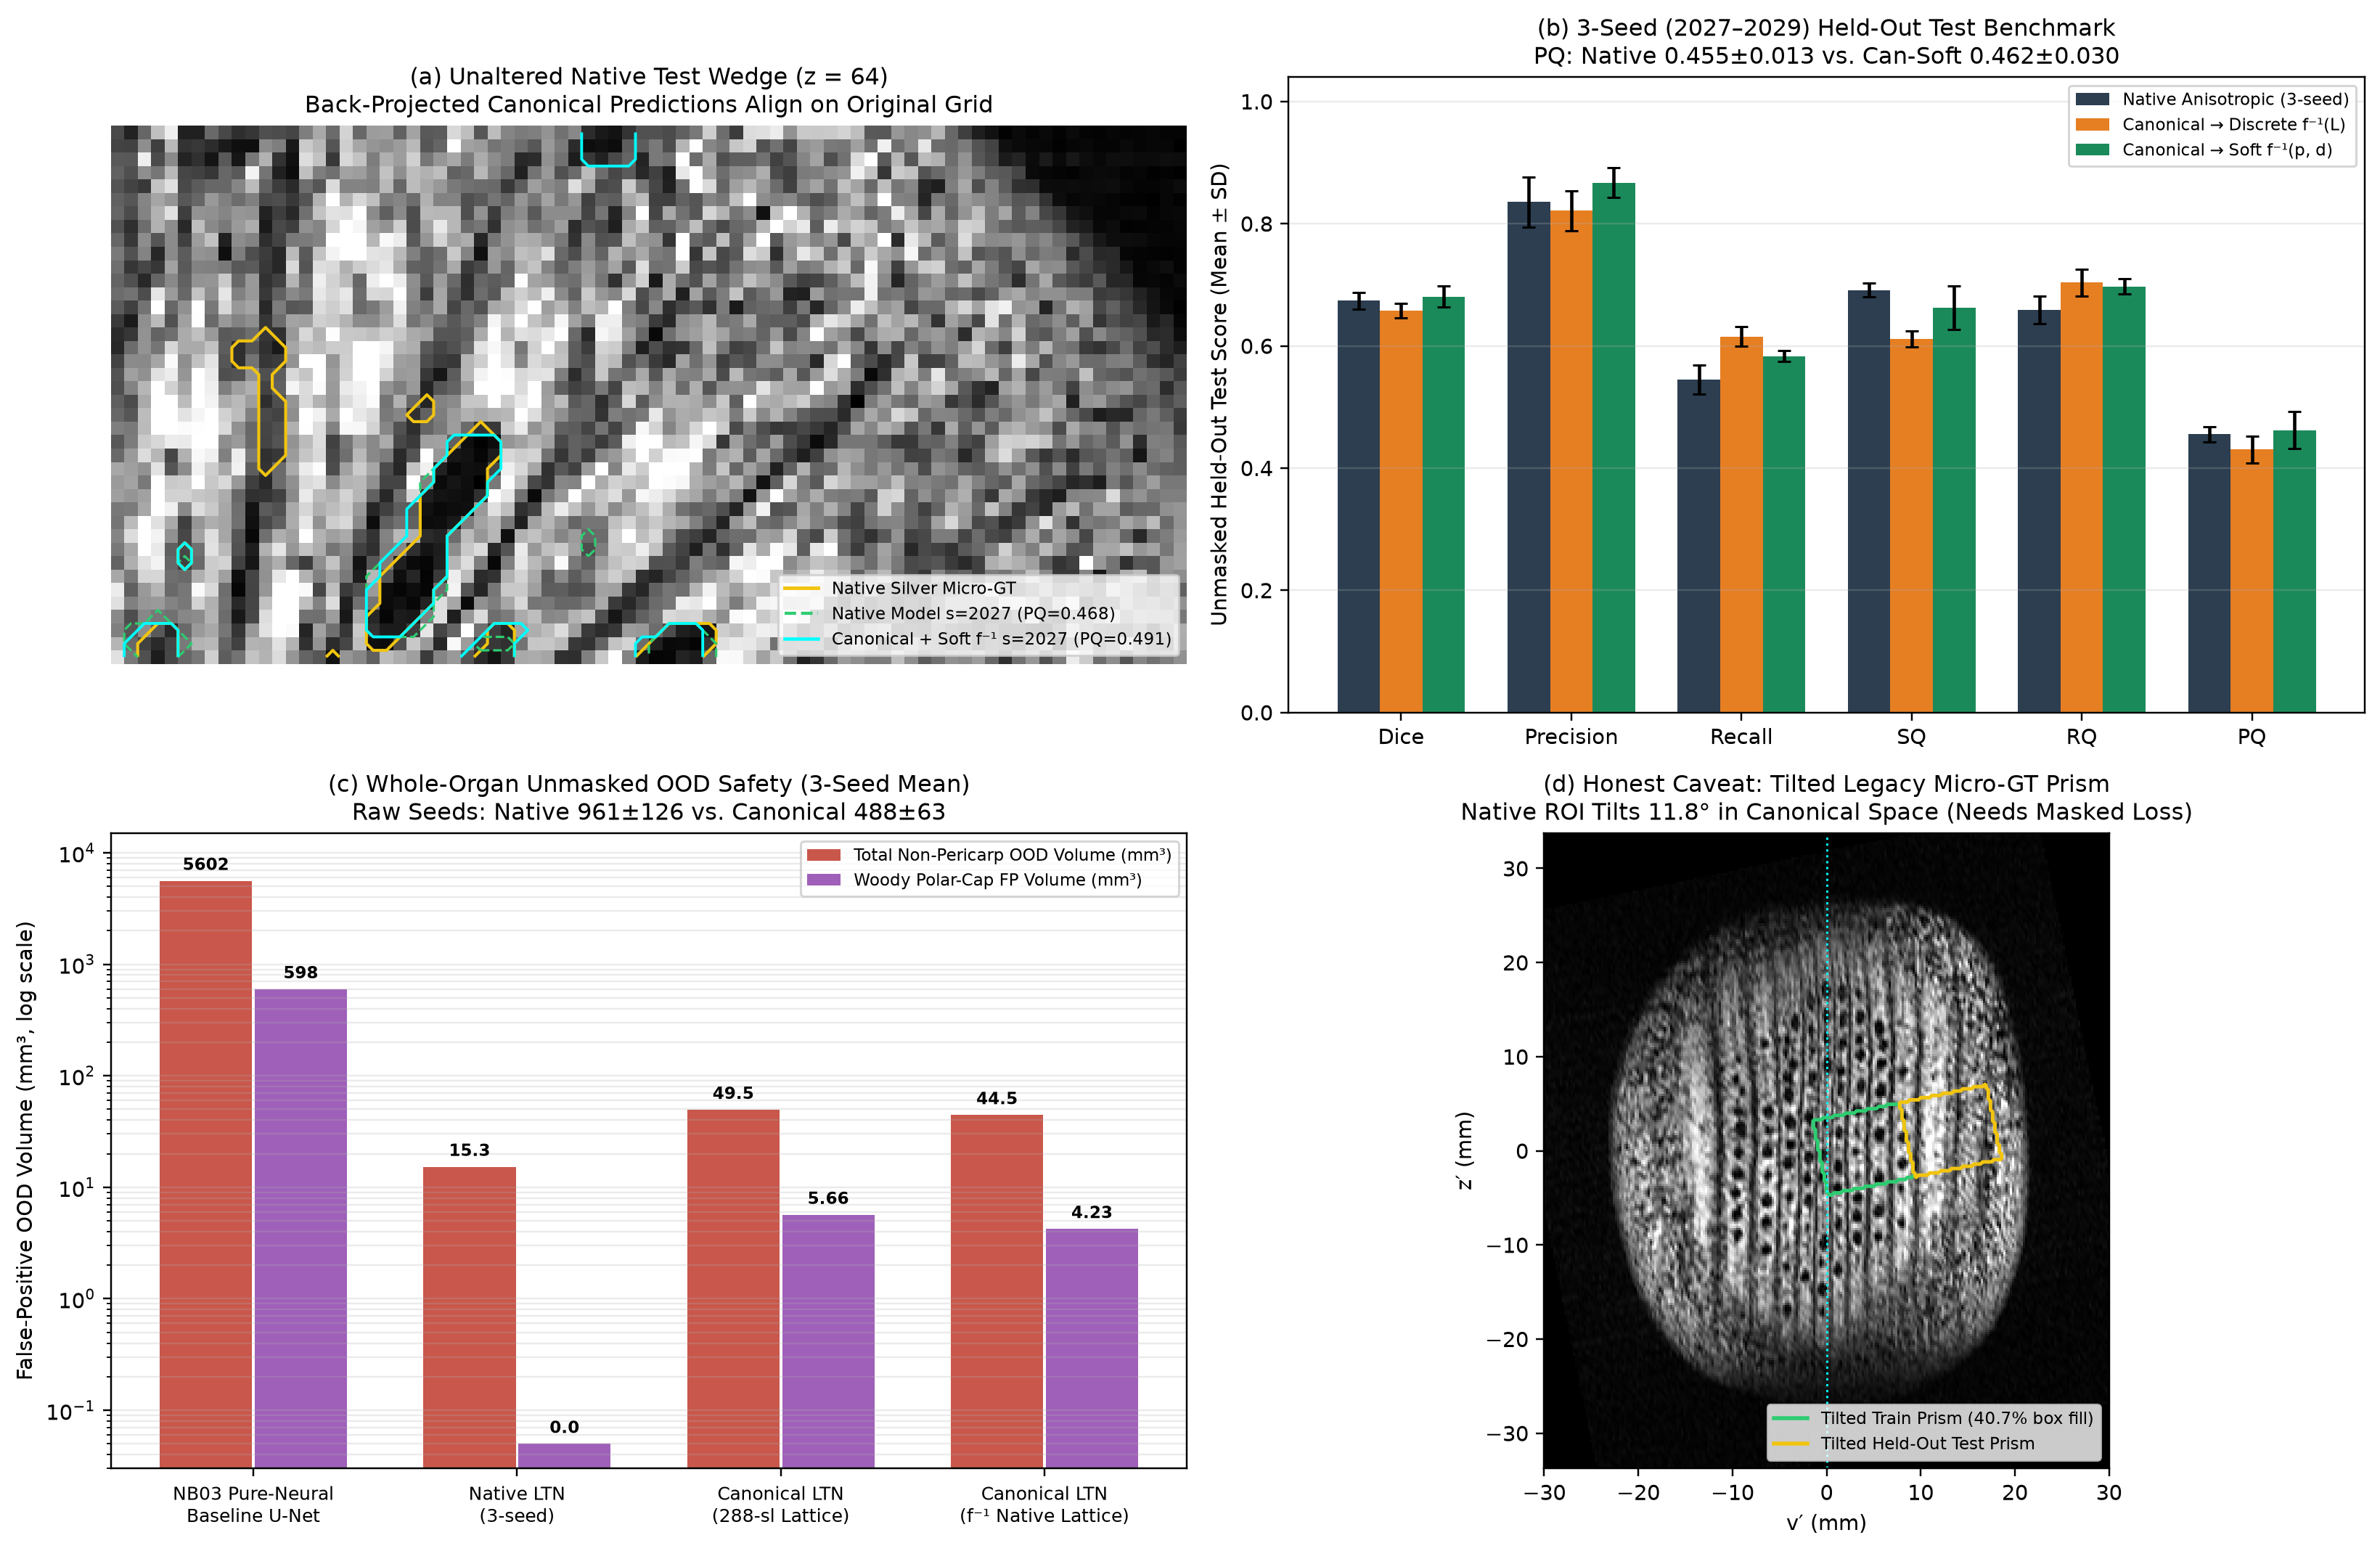
\includegraphics[width=\textwidth]{../figures/fig00e_canonical_segmentation_roundtrip.png}
    \vspace{-4pt}
    \caption*{\footnotesize\textit{Executed Figure~0e (\texttt{Out [6]}, saved as \texttt{fig00e\_canonical\_segmentation\_roundtrip.png}): (a) Back-projected canonical predictions aligned on unaltered native Test Wedge ($z = 64$); (b) 3-seed mean $\pm$ SD held-out metrics; (c) unmasked whole-organ OOD safety ($\text{mm}^3$, log scale) vs.\ NB~03 pure-neural baseline U-Net; (d) $11.8^\circ$-tilted legacy Micro-GT prism caveat in canonical sagittal view.}}
\end{figure}

\section*{6. Synthesis, Workflow Recommendations \& Optional Canonical NIfTI Export (\texttt{MyStuff/})}
\addcontentsline{toc}{section}{\texorpdfstring{6. Synthesis, Recommendations \& Optional NIfTI Export}{6. Synthesis and Optional NIfTI Export}}

\begin{clinbox}[Practical Decision Guide: When to Use Canonical Isotropic N--S Space ($f = f_2 \circ f_1$)]
\begin{itemize}
    \item \textbf{Manual 3D Curation (\texttt{freeview} / \texttt{ITK-SNAP} / \texttt{3D Slicer} / NB~03b):} \textit{Strongly favors Canonical \texttt{0.2344$^3$\,mm$^3$}}. Seeds become isotropic ($7\times 6\times 7$ voxels), coronal/\allowbreak{}sagittal staircasing vanishes, scrolling $z'$ has zero lateral drift, and back-projection via $f^{-1}$ recovers \texttt{98/98} seeds (\texttt{Dice = 0.984, PQ@0.50 = 0.967}) and \texttt{749/749} whole-fruit seeds (\texttt{PQ@0.50 = 0.968}) bit-aligned to the original NIfTI \texttt{sform}.
    \item \textbf{Botanical Visualization, QC \& Symbolic \texttt{Organ-GPS} Priors:} \textit{Strongly favors Canonical N--S space}. Carpel slant drops by $>50\%$ ($3.49^\circ \to 1.71^\circ$), slice concentricity error drops by 56.1\%, and cylindrical Mercator unrolling displays all carpel meridians at a single glance.
    \item \textbf{3D Neurosymbolic Deep Learning (3-Seed Findings):} Always use \textbf{continuous probability/\allowbreak{}distance pullback} $f^{-1}(\hat{p}, \hat{d})$ rather than discrete \texttt{order=0} label pullback when projecting canonical neural predictions back to native space (3-seed PQ: \texttt{0.462 $\pm$ 0.030} vs.\ discrete \texttt{0.430 $\pm$ 0.022} and native \texttt{0.455 $\pm$ 0.013}; whole-organ OOD remains near-zero across both frames vs.\ \texttt{5,602\,mm$^3$} for the pure-neural baseline). Note the $\approx 2.1\times$ training compute trade-off (\texttt{48.7\,s} vs.\ \texttt{22.9\,s}) and \texttt{40.7\%} legacy tilted-prism overhead---eliminated when new ROIs are curated upright in canonical space.
\end{itemize}
\end{clinbox}

\begin{codebox}[{In [7] $\cdot$ Python --- In-memory NIfTI \texttt{sform}/\texttt{qform} audit \& optional \texttt{MyStuff/} export}]
\begin{lstlisting}[style=pybmed]
# Toggle to True to write git-ignored canonical NIfTI files into MyStuff/kiwi-canonical/
EXPORT_CANONICAL_NIFTI = False

# Always verify NIfTI sform/qform header integrity in memory (zero disk bloat)
mri_c_img = nib.Nifti1Image(vol_canon.astype(np.float32), A_canon)
mri_c_img.set_sform(A_canon, code=1)
mri_c_img.set_qform(A_canon, code=1)

gt_c_img = nib.Nifti1Image(gt_c_sdf.astype(np.uint16), A_canon)
gt_c_img.set_sform(A_canon, code=1)
gt_c_img.set_qform(A_canon, code=1)

rt_native_img = nib.Nifti1Image(gt_rt_nn.astype(np.uint16), A_orig)
rt_native_img.set_sform(A_orig, code=1)
rt_native_img.set_qform(A_orig, code=1)

print("In-memory NIfTI header verification:")
print(f"  Canonical MRI vs Canonical GT affine max diff : {float(np.max(np.abs(mri_c_img.affine - gt_c_img.affine))):.6f} (BIT-IDENTICAL)")
print(f"  Round-trip GT vs Original MRI affine max diff : {float(np.max(np.abs(rt_native_img.affine - A_orig))):.6f} (BIT-IDENTICAL)")
print(f"  Canonical voxel zooms (mm)                    : {tuple(round(float(z), 6) for z in mri_c_img.header.get_zooms()[:3])}")

if EXPORT_CANONICAL_NIFTI:
    repo_root = next((p for p in [Path.cwd(), *Path.cwd().parents] if (p / "pyproject.toml").exists()), Path.cwd())
    out_dir = repo_root / "MyStuff" / "kiwi-canonical"
    out_dir.mkdir(parents=True, exist_ok=True)
    p_mri = out_dir / "kiwi_7T_canonical_iso_NS.nii.gz"
    p_gt = out_dir / "kiwi_micro_gt_canonical_sdf_cubic.nii.gz"
    p_wf = out_dir / "kiwi_neurosymbolic_pred_canonical_nn.nii.gz"
    p_rt = out_dir / "kiwi_micro_gt_roundtrip_native.nii.gz"
    p_xfm = out_dir / "kiwi_canonical_transform_f2_o_f1.json"

    nib.save(mri_c_img, str(p_mri))
    nib.save(gt_c_img, str(p_gt))
    kns.save_aligned_label_nifti(wf_c_nn, A_canon, p_wf)
    nib.save(rt_native_img, str(p_rt))
    p_xfm.write_text(json.dumps({
        "A_orig": A_orig.tolist(),
        "A_canon": A_canon.tolist(),
        "T_f2_world": T_f2.tolist(),
        "M_canon_to_orig": M_c2o.tolist(),
        "M_orig_to_canon": M_o2c.tolist(),
    }, indent=2), encoding="utf-8")

    lut_rel = "Lab4-Comp-Imag/Kiwi-challenge/scripts/kiwi_seeds_ColorLUT.txt"
    print(f"\nExported git-ignored canonical volumes to: {out_dir}")
    print("Launch in FreeSurfer freeview (macOS):")
    print(f"  /Applications/freesurfer/8.2.0/bin/freeview \\")
    print(f"    -v {p_mri}:colormap=grayscale:percentile=1:grayscale=0,99.5 \\")
    print(f"    -v {p_gt}:colormap=lut:lut={repo_root / lut_rel}:opacity=0.58 \\")
    print(f"    -v {p_wf}:colormap=lut:lut={repo_root / lut_rel}:opacity=0.45:visible=0")
else:
    print("\nTip: Set EXPORT_CANONICAL_NIFTI = True above to write canonical NIfTI files to git-ignored MyStuff/kiwi-canonical/.")
\end{lstlisting}
\end{codebox}
\begin{outbox}[{Out [7] $\cdot$ stdout}]
\begin{lstlisting}[style=outbmed]
In-memory NIfTI header verification:
  Canonical MRI vs Canonical GT affine max diff : 0.000000 (BIT-IDENTICAL)
  Round-trip GT vs Original MRI affine max diff : 0.000000 (BIT-IDENTICAL)
  Canonical voxel zooms (mm)                    : (0.234375, 0.234375, 0.234375)

Tip: Set EXPORT_CANONICAL_NIFTI = True above to write canonical NIfTI files to git-ignored MyStuff/kiwi-canonical/.
\end{lstlisting}
\end{outbox}

\end{document}
